% class options:
% - select either [german] or [english]
% - select the type of thesis from:
%   [bachelor, master, generic]
%   (in case of generic, use \type{} to specify it)
% - use option "alpha" for abbreviated citation (instead of numbers)
% - option "draft" is available, too
% - use options "utf8" or "latin1" to select inputencoding
\documentclass[german, master, utf8]{base/thesis_KBS}

\addbibresource{lib.bib}

\usepackage{units}    % useful for settings units:              \unit[23]{m}
\usepackage{nicefrac} % for setting fractions esp. within text: \nicefrac{km}{h}

\usepackage{algorithm, algorithmic}  % for pseudo code (cf. documentation)
\usepackage{tikz}
\renewcommand{\algorithmiccomment}[1]{\qquad{\small // \textit{#1}}}

\renewcommand{\lstlistingname}{Quellcode}% Listing -> Quellcode
\newcommand{\lstlistingautorefname}{Quellcode}% Listing -> Quellcode

%\bibliography{library}
\newglossary[tlg]{symbols}{tld}{tdn}{Symbol Verzeichnis}

\makeglossaries

%%%%%%%%%%%%%%%%%%%%%%%%%%%%%%%%%%%%%%%%%%%%%%%%%%%%%%%%%%%%%%%%%%%%%%%%%%%%%%%%%%%%%%%%%%%%%%%%%%%
% Fachwörter starting here
% use g for doubles entries in Abkürzungen und Fachwörter
%%%%%%%%%%%%%%%%%%%%%%%%%%%%%%%%%%%%%%%%%%%%%%%%%%%%%%%%%%%%%%%%%%%%%%%%%%%%%%%%%%%%%%%%%%%%%%%%%%%
\newglossaryentry{annotationen}{
  name = {Annotationen},
  sort = {Annotationen},
  description = {Tupel aus Label und Segmentmarkierung. Die Markierung bezieht sich auf einen Auschnitt innerhalb eines ungeschnittenen Videos und das Label gibt eine in diesem Ausschnitt stattfindende Aktion an.}
}
\newglossaryentry{backpropagation}{
  name = {Backpropagation},
  sort = {Backpropagation},
  description = {}
}
\newglossaryentry{bottleneck}{
  name = {Bottleneck},
  sort = {Bottleneck},
  description = {}
}
\newglossaryentry{channel}{
  name = {Kanal},
  sort = {Kanal},
  plural = {Kanäle},
  description = {}
}
\newglossaryentry{clip}{
  name = {Clip},
  sort = {Clip},
  description = {Ausschnitt fester Länge aus einem ungeschnittenen Video}
}
\newglossaryentry{dataset}{
  name = {Datenset},
  sort = {Datenset},
  description = {Datentupel aus Beispiel und Label}
}
\newglossaryentry{deep-learning}{
  name ={Deep Learning},
  sort = {Deep Learning},
  description = {}
}
\newglossaryentry{neural-nets}{
  name ={Neuronale Netze},
  sort = {Neuronale Netze},
  description = {}
}
\newglossaryentry{feature}{
  name = {Feature},
  sort = {Feature},
  description = {todo: The key point for low level feature are corners, edges, blobs or contours while high level feature is
more holistic like the structured information related to the action being taken}
}
\newglossaryentry{feature-map}{
  name = {Feature Map},
  sort = {Feature Map},
  description = {todo: }
}
\newglossaryentry{frames}{
  name = {Frames},
  sort = {Frames},
  description = {todo: }
}
\newglossaryentry{hyperparameter}{
  name = {Hyperparameter},
  sort = {Hyperparameter},
  description = {todo: A hyperparameter is a property of a learning algorithm, usually (but not always) having a numerical value.
That value influences the way the algorithm works and is not learned from the algorithm itself.}
}
\newglossaryentry{kernel}{
  name = {Kernel},
  sort = {Kernel},
  description = {todo:}
}
\newglossaryentry{label}{
  name = {Label},
  sort = {Label},
  description = {todo: a member of a finite set of classes}
}
\newglossaryentry{layer}{
  name = {Layer},
  sort = {Layer},
  description = {Schicht aus Knoten innerhalb eines Neuronalen Netzes}
}
\newglossaryentry{moving-window}{
  name = {Moving Window},
  sort = {Moving Window},
  description = {todo:}
}
\newglossaryentry{optical-flow}{
  name = {Optischer Fluss},
  sort = {Optischer Fluss},
  description = {Der optische Fluss einer Bildsequenz ist das Vektorfeld der in die Bildebene projizierten Geschwindigkeit von sichtbaren Punkten des Objektraumes im Bezugssystem der Abbildungsoptik}
}
\newglossaryentry{overfitting}{
  name = {Overfitting},
  sort = {Overfitting},
  description = {Überanpassung der Netz-Parameter an die Trainingsdaten:
    Das Netz hat während des Trainings zu viele Freiheitsgrade, sodass es nicht korrekt abstrahiert, sondern beginnt Beispiele auswendig zu lernen.}
}
\newglossaryentry{pooling}{
  name = {Pooling},
  sort = {Pooling},
  description = {todo:}
}
\newglossaryentry{rgb}{
  name ={RGB},
  sort = {RGB},
  description = {Additives Farbmodell zur Kodierung von Farbwerten aus drei Lichtkanälen (rot, grün und blau)}
}
\newglossaryentry{sample}{
  name = {Sample},
  sort = {Sample},
  description = {Datensatz aus Clip und Labels $(x_i, y_i)$}
}
\newglossaryentry{training}{
  name = {Training},
  sort = {Training},
  description = {}
}
\newglossaryentry{transfer-learning}{
  name = {Transfer Learning},
  sort = {Transfer Learning},
  description = {}
}
\newglossaryentry{vanish-gradient}{
  name = {Vanishing Gradient Problem},
  sort = {Vanishing Gradient Problem},
  description = {}
}


%%%%%%%%%%%%%%%%%%%%%%%%%%%%%%%%%%%%%%%%%%%%%%%%%%%%%%%%%%%%%%%%%%%%%%%%%%%%%%%%%%%%%%%%%%%%%%%%%%%
% Acronyms starting here
% Anmerkung: Nicht wundern - selbe Anfangsbuchstaben rücken näher zusammen im Verzeichnis
% http://tug.ctan.org/tex-archive/macros/latex/contrib/glossaries/glossariesbegin.html#sec:xr
%%%%%%%%%%%%%%%%%%%%%%%%%%%%%%%%%%%%%%%%%%%%%%%%%%%%%%%%%%%%%%%%%%%%%%%%%%%%%%%%%%%%%%%%%%%%%%%%%%%

\newacronym{api}{API}{Application Programming Interface}
\newacronym{cnn}{CNN}{Convolutional Neural Network}
\newacronym{csv}{CSV}{Comma-Separated Values}
\newacronym{dnn}{DNN}{Deep Neural Networks}
\newacronym{flops}{FLOPS}{Floating Point Operations per Second}
\newacronym{fps}{Fps}{Frames per second}
\newacronym{gpu}{GPU}{Graphics Processing Unit}
\newacronym{gui}{GUI}{Graphical User Interface}
\newacronym{har}{HAR}{Human Action Recognition}
\newacronym{idt}{iDT}{improved Dense Trajectories}
\newacronym{json}{JSON}{JavaScript Object Notation}
\newacronym[see={[Glossar:]{training}}]{ml}{ML}{Machine Learning}
\newacronym{mlp}{MLP}{Multi-Layer Perceptron}
\newacronym{mse}{MSE}{Mean squared error}
\newacronym{ocr}{OCR}{Object Character Recognition}
\newacronym{pca}{PCA}{Hauptkomponentenanalyse}
\newacronym{pes}{PES}{Packetized elementary stream}
\newacronym{pts}{PTS}{Presentation timestamps}
\newacronym{relu}{ReLU}{Rectified Linear Unit}
\newacronym{rnn}{RNN}{Recurrent Neural Network}
\newacronym{sbod}{SBOD}{StatsBomb Open Data}
\newacronym{svm}{SVM}{Support Vector Machine}
\newacronym[see={[Kapitel:]{sec:temporal-action-detection}}]{tsn}{TSN}{Temporal Segment Network}
\newacronym{url}{URL}{Uniform Resource Locator}

%%%%%%%%%%%%%%%%%%%%%%%%%%%%%%%%%%%%%%%%%%%%%%%%%%%%%%%%%%%%%%%%%%%%%%%%%%%%%%%%%%%%%%%%%%%%%%%%%%%
% Symbols starting here
%%%%%%%%%%%%%%%%%%%%%%%%%%%%%%%%%%%%%%%%%%%%%%%%%%%%%%%%%%%%%%%%%%%%%%%%%%%%%%%%%%%%%%%%%%%%%%%%%%%

\newglossaryentry{tld:A}{%
	type=symbols,
	name={A},
	description={Anzahl möglicher Aktionsklassen (Labels)}
}
\newglossaryentry{tld:C}{%
	type=symbols,
	name={C},
	description={Anzahl Kanäle}
}
\newglossaryentry{tld:D}{%
	type=symbols,
	name={D},
	description={Set aus Datensamples}
}
\newglossaryentry{tld:S}{%
	type=symbols,
	name={S},
	description={Räumliche Auflösung}
}
\newglossaryentry{tld:T}{%
	type=symbols,
	name={T},
	description={Anzahl der Frames, zeitliche Auflösung}
}


\newglossaryentry{tld:b}{%
	type=symbols,
	name={b},
	description={Bias eines Layers}
}
\newglossaryentry{tld:d}{%
	type=symbols,
	name={d},
	description={Kerneldimension (temporärer Achse)}
}
\newglossaryentry{tld:i}{%
	type=symbols,
	name={i},
	description={Index eines Samples}
}
\newglossaryentry{tld:k}{%
	type=symbols,
	name={k},
	description={Kerneldimension (räumliche Achsen)}
}
\newglossaryentry{tld:l}{%
	type=symbols,
	name={l},
	description={Layer-Index}
}
\newglossaryentry{tld:r}{%
	type=symbols,
	name={r},
	description={Verhältnis von Samples einer Klasse zu der Gesamtzahl an Samples}
}
\newglossaryentry{tld:u}{%
	type=symbols,
	name={u},
	description={Zellenindex eines Neurons innerhalb eines Layers}
}
\newglossaryentry{tld:w}{%
	type=symbols,
	name={w},
	description={Gewicht}
}
\newglossaryentry{tld:x}{%
	type=symbols,
	name={x},
	description={Input-Vektor $x \in \mathbb{R}^{(C \times T \times S^2)}$, enthält Clip eines Samples}
}
\newglossaryentry{tld:y}{%
	type=symbols,
	name={y},
	description={Output-One-Hot-Vektor $y \in \{0, 1\}^A$ enthält Labels eines Samples}
}

\newglossaryentry{tld:Delta}{%
	type=symbols,
	name={\Delta},
	description={Dauer eines Clips (Clip-Abdeckung)}
}
\newglossaryentry{tld:sigma}{%
	type=symbols,
	name={$\sigma$},
	description={Aktivierungsfunktion}
}
\newglossaryentry{tld:gamma-tau}{%
	type=symbols,
	name={\gamma_\tau},
	description={Samplingrate: $\tau = 1$ entspricht Original-Framerate}
}
\newglossaryentry{tld:gamma-lambda}{%
	type=symbols,
	name={$\Lambda$},
	description={temporal coverage}
}
\newglossaryentry{tld:Psi}{%
	type=symbols,
	name={\Psi},
	description={Menge der Scores pro gesampleten Clips}
}
\newglossaryentry{tld:theta}{%
	type=symbols,
	name={$\theta$},
	description={Grenzwert}
}
\newglossaryentry{tld:Theta}{%
	type=symbols,
	name={\Theta},
	description={Obergrenze}
}

% Symbols
\newcommand{\cmark}{\ding{51}}  % checkmark
\newcommand{\xmark}{\ding{55}}  % xmark

% Quotes
\newcommand{\inquotes}[1]{{{\glqq}#1{\grqq}}} % quotes
\newcommand{\qq}{\symbol{34}} % ASCII char double quotes
\newcommand{\qqqq}{\qq\qq} % double double quotes (= empty string)

% Namings
\renewcommand{\subsectionautorefname}{Abschnitt}
\renewcommand{\subsubsectionautorefname}{Abschnitt}

% Fonts
\renewcommand{\familydefault}{\sfdefault}
%\renewcommand{\sectfont}{\large\sffamily\bfseries\color{dark-gray}}

% Highlight
\newcommand{\code}[1]{\texttt{#1}}

% misc
\newcommand{\watermark}[1]{\AddToShipoutPictureBG{%
    \AtPageCenter{
        \rotatebox{15}{
            \makebox[0pt]{%
                \Huge\bfseries\color{red}#1
            }
        }
    }%
}}

% graphics
\newcommand{\bigimage}[2]{
    \includegraphics[width=#2, height=#2, keepaspectratio, interpolate]{#1}
}

\newcommand{\smallimage}[1]{
    \includegraphics[width=2cm, height=2cm, keepaspectratio, interpolate]{#1}
}

\newcommand{\titledimage}[2]{
    \stackinset{l}{1em}{t}{1em}
        {\colorbox{yellow}{#2}}
        {\includegraphics[width=0.5\textwidth]{#1}}
}

\newcommand{\imgfigure}[3]{
    \begin{figure}[htbp!]
        \centering
        \bigimage{#1}{0.9\textwidth}
        \caption{#2}
        \label{#3}
    \end{figure}
}

% tables
%\rowcolors[]{2}{gray!15}{white} % possible option \hline

\newcommand{\head}[1]{
    \cellcolor{black!75}
    \textcolor{white}{
        \textbf{#1}
    }
}

\newcommand{\headline}{ % Todo: coloring not working...
    \rowcolor{black!75}
    \rowfont{\color{white}}
}

\renewcommand{\arraystretch}{1.5}

% algorithm
\newcommand{\minbox}[2]{%
  \mathmakebox[\ifdim#1<\width\width\else#1\fi]{#2}}
\newcommand{\Let}[2]{\State $ \minbox{1em}{#1} \gets #2 $}

% abbreviations
\newcommand{\iA}{i.\ A.\ }
\newcommand{\ZB}{Z.\ B.\ }
\newcommand{\zB}{z.\ B.\ }
\newcommand{\Bspw}{Bspw.\ }
\newcommand{\bspw}{bspw.\ }
\newcommand{\bzgl}{bzgl.\ }
\newcommand{\vgl}{vgl.\ }
\newcommand{\bzw}{bzw.\ }
\newcommand{\etc}{etc.\ }
\newcommand{\oAe}{o.\ Ä.\ }
\newcommand{\oae}{o.\ ä.\ }
\newcommand{\uU}{u.\ U.\ }
\newcommand{\Dh}{D.\ h.\ }
\renewcommand{\dh}{d.\ h.\ }
\newcommand{\ua}{u.\ a.\ }
\newcommand{\ggf}{ggf.\ }
\newcommand{\sog}{sog.\ }

\newcommand{\fc}{\emph{fc}}
\newcommand{\pool}{\emph{pool}}
\newcommand{\conv}{\emph{conv}}
\newcommand{\res}{\emph{res}}
\newcommand{\stem}{\emph{stem}}

\definecolor{eclipseStrings}{RGB}{42,0.0,255}
\definecolor{eclipseKeywords}{RGB}{127,0,85}
\colorlet{numb}{magenta!60!black}

\lstset{
  basicstyle=\lst@ifdisplaystyle\footnotesize\fi\ttfamily, % the size of the fonts that are used for the code
  breakatwhitespace=false,           % sets if automatic breaks should only happen at whitespace
  breaklines=true,                   % sets automatic line breaking
  captionpos=b,                      % sets the caption-position to bottom
  escapeinside={\%*}{*)},            % if you want to add LaTeX within your code
  extendedchars=true,                % lets you use non-ASCII characters; for 8-bits encodings only, does not work with UTF-8
  %frame=single,	                     % adds a frame around the code
  keepspaces=true,                   % keeps spaces in text, useful for keeping indentation of code (possibly needs columns=flexible)
  numbers=none,                      % where to put the line-numbers; possible values are (none, left, right)
  numbersep=8pt,                     % how far the line-numbers are from the code
  %rulecolor=\color{black},           % if not set, the frame-color may be changed on line-breaks within not-black text (e.g. comments (green here))
  showspaces=false,                  % show spaces everywhere adding particular underscores; it overrides 'showstringspaces'
  showstringspaces=false,            % underline spaces within strings only
  showtabs=false,                    % show tabs within strings adding particular underscores
  stepnumber=2,                      % the step between two line-numbers. If it's 1, each line will be numbered
  tabsize=4,	                     % sets default tabsize to 2 spaces
  title=\lstname,                    % show the filename of files included with \lstinputlisting; also try caption instead of title
  %backgroundcolor=\color{white},
  commentstyle=\color{green!60!black},
  keywordstyle=\color{blue},
  numberstyle=\scriptsize\color{black},
  stringstyle=\color{red!70!blue}
}

\lstdefinelanguage{json}{
    numbers=none,
    basicstyle=\normalfont\ttfamily,
    commentstyle=\color{eclipseStrings}, % style of comment
    stringstyle=\color{eclipseKeywords}, % style of strings
    numbers=left,
    numberstyle=\scriptsize,
    stepnumber=1,
    numbersep=8pt,
    showstringspaces=false,
    breaklines=true,
    %frame=lines,
    backgroundcolor=\color{white}, %only if you like
    string=[s]{"}{"},
    comment=[l]{:\ "},
    morecomment=[l]{:"},
    literate=
        *{0}{{{\color{numb}0}}}{1}
         {1}{{{\color{numb}1}}}{1}
         {2}{{{\color{numb}2}}}{1}
         {3}{{{\color{numb}3}}}{1}
         {4}{{{\color{numb}4}}}{1}
         {5}{{{\color{numb}5}}}{1}
         {6}{{{\color{numb}6}}}{1}
         {7}{{{\color{numb}7}}}{1}
         {8}{{{\color{numb}8}}}{1}
         {9}{{{\color{numb}9}}}{1}
}

\usepackage{draftwatermark}
\SetWatermarkText{Draft}
\SetWatermarkScale{1.5}
\SetWatermarkColor[gray]{0.8}

%%%%%%%%%%%%%%%%%%%%%%%%%%%%%%%%%%%%%%%%%%%%%%%%%%%%%%%%%%%%%%%%%%%%%%%%%%%%%%%
\usepackage{tablefootnote}

\begin{document}

\title{Deep-Learning-basierte Klassifikation von Spielaktionen in Fußballvideos}
\author{Simon Narendorf}
\email{snarendorf@uni-osnabrueck.de}
\firstSupervisor{Prof. Dr. Joachim Hertzberg}
\secondSupervisor{Dr. Isabel Hübener}
%\shorttitle{...}                       % by default = title
%\dept{...}                             % by default KBS UOS
%\submitdate{November 2004}             % by default current month & year
%\signcity{}                            % by default Osnabr�ck
%signline{Osnabr�ck, 11. Dezember 2004} % by default "signcity, submitdate"

\generatetitle

\cleardoublepage

\newcommand{\primarymetric}{66,1}
\newcommand{\secondarymetric}{72,8}

\begin{prefacesection}{Abstract}
    Die Erkennung von Aktionen in Videos, auch \gls{har} genannt, ist Gegenstand aktueller Forschung im Bereich Video Understanding.
    Großspurige Datensets beschränken sich meist auf allgemeine, Domänen-übergreifende Klassen, die eindeutig voneinander abgrenzbar sind und nicht in Kombination auftreten.
    Hingegen finden im Bereich von Feldsportarten, wie Fußball, oft viele, visuell ähnliche Aktionen in kürzester Zeit oder sogar zeitgleich statt.
    Die bestehenden Datensets dieser Domäne bilden bislang nur einen Bruchteil der Spielaktionen aus der realen Welt ab.
    Hier knüpft die vorliegende Arbeit an, in der ein Multi-Label-Datenset mit insgesamt 32 verschiedenen Aktionsklassen, basierend auf TV-Aufzeichnungen von Fußballspielen, neu generiert wird.
    In anschließenden Benchmarks kommen verschiedene Deep-Learning-Architekturen (R2+1D, SlowFast, ir-CSN) als Video-Klassifizierer zum Einsatz, die anhand des neuen Datensets mit Methoden des Transfer-Learnings und ohne weitere Zwischenschritte (\emph{Ende-zu-Ende}) trainiert werden.
    Die Ergebnisse zeigen, dass aktuelle Modelle des Deep-Learnings bereits in der Lage sind, einen Großteil der 32 Klassen hinreichend gut zu erkennen.
    Im Vergleich erreicht ir-CSN hierbei die besten Ergebnisse -- mit einer Balanced Accuracy von \primarymetric \% (\secondarymetric \% bei 24 Klassen).

    \begin{tcolorbox}[title=WIP]
        Weitere Key-Findings: Auflösung und Geschwindigkeit der Videos erwähnen, BA updaten
    \end{tcolorbox}

    The recognition of actions in videos (also Human Action Recognition (HAR)) is the subject of current research in the field of video understanding.
    Large-scale data sets are mostly limited to general, cross-domain classes that are clearly distinguishable from one another and do not occur in combination.
    On the other hand, in the domain of field sports, such as soccer, visually similar actions often take place in a very short time or even at the same time.
    Existing datasets of this domain so far represent only a fraction of the actions from the real world.
    This is where the thesis starts by creating a multi-label dataset with a total of 32 different action classes included, based on TV recordings of soccer matches.
    In the subsequent benchmarks, various Deep Learning architectures (R2+1D, SlowFast, ir-CSN) are used as video classifiers, which are trained end-to-end on the new dataset with methods of transfer learning and without further intermediate steps.
    The results show that current Deep Learnings models are already able to recognize a large part of the 32 classes sufficiently well.
    In comparison, ir-CSN achieved the best results - with a balanced accuracy of \primarymetric \% (\secondarymetric \% in 24 classes).

\end{prefacesection}

\cleardoublepage
\tableofcontents


\startTextChapters %%%%%%%%%%%%%%%%%%%%%%%%%%%%%%



\chapter{Einleitung}
\label{ch:intro}

Die automatisierte Klassifizierung von Videomaterial ist im Alltag vieler Menschen ein fester Bestandteil.
Auswertungen von Überwachungskameras, Gesten-Steuerung an Smartphones und Erkennung von Müdigkeit am Steuer sind nur einige Beispiele.
Der Sport- und im Speziellen der Fußballsektor ist besonders gekennzeichnet durch eine hohe Anzahl öffentlich verfügbarer Videos~\cite{Giancola18}, aus denen neues Wissen abgeleitet werden kann.
Diese Arbeit beschäftigt sich in diesem Zusammenhang mit der Erkennung atomarer, wohl-definierter Spielaktionen, wie Torschüsse, Auswechslungen oder Fouls, die eine spezielle Form der \gls{har} ist.
Die Spielaktionen sollen effizient und ausschließlich anhand des zugrunde liegenden Videobilds erkannt werden.

Der Einsatz von Deep-Learning im Bereich der Video-Klassifizierung (\gls{har}) führte in den letzten Jahren zu einem signifikanten Fortschritt~\cite{Abu-Bakar19}.
Besonders durch die Verfügbarkeit von \glspl{gpu} und den Veröffentlichungen neuer umfassender Datensets konnten die Erkennungsraten in den letzten Jahren deutlich verbessert werden. % todo: quelle

In der Sportdomäne ergeben sich besondere technische Herausforderungen in der Erkennung von Spielaktionen -- vor allem durch die Ähnlichkeit der Videos.
Man spricht in diesem Zusammenhang von einer besonders hohen Inter-Klassen-Ähnlichkeit (inter-class similarity), die sich dadurch auszeichnet, dass verschiedene Klassen ähnliche visuelle Merkmale aufweisen, sich jedoch semantisch unterscheiden~\cite{Sozykin17}.
Dazu kommt eine besonders hohe Intra-Klassen-Varianz (intra-class variance)~\cite{Ballan09}, \dh verschiedene Samples der gleichen Klassen können einen sehr unterschiedlichen Verlauf haben.
Weitere Herausforderungen sind die Ungleichverteilung (imbalance) der Aktionsklassen, sowie die potenzielle Überschneidung von Klassen~\cite{Jiang19}.

\section{Motivation}
\label{sec:motivation}

Im Fußball-Scouting sind Spieldaten eine begehrte Ressource.
Vor allem die Auswertung von Videomaterial aus TV-Aufzeichnungen erfordert jedoch viel Zeit.
Dazu werden Spiele meist manuell mit Markierungen zu den Spielaktionen, wie Tore, Auswechslungen oder Zweikämpfen versehen.
Diese Markierungen, im Folgenden \gls{annotationen} genannt, bestehen aus einem Label (entspricht der Aktionsklasse), sowie einer Start- und Endzeit, die den Zeitraum im Video definieren, in der die Aktion stattfindet.

Die \gls{annotationen} gelten im Kontext der Klassifikation als die \sog verifizierte Ground Truth.
Praktischen Einsatz erlangen derartige \gls{annotationen} auch im Scouting.
Fußball-Scouts können \zB effizienter an einer qualitativen Video-Analyse arbeiten, wenn sie wissen an welchen Stellen im Video, die für sie interessanten Aktionen stattfinden.

Das Annotieren selbst ist allerdings ein zeitaufwendiger, teuer und monotoner Prozess.
Spieldaten werden meist von freiwilligen Datenpflegern einer Community-Website oder von professionellen Datenpflegern erfasst.
Datenprovider wie Wyscout, stellen bis zu 400 Vollzeitressourcen ein, die pro Spiel bis zu 2000 \gls{annotationen} beisteuern können~\cite{Jiang19}.

Diese Arbeit optimiert zunächst mittels existierender Modelle die Klassifikation von hand-annotierten Spielaktionen.
Dadurch soll ermöglicht werden, dass derartige \gls{annotationen} künftig für den produktiven Einsatz im Scouting voll- oder teil-automatisiert generiert werden können und der manuelle Aufwand reduziert wird.

\section{Problemstellung und Forschungsfrage}
\label{sec:forschungsfrage}

In der Fußballdomäne gibt es zurzeit nur kleine oder unvollständige Datensets~\cite{Giancola18, Jiang19}.
Darüber hinaus sind die Erkennungsraten bei der Anwendung auf diesen Datensets vergleichsweise gering verglichen mit den groß angelegten, generischen Datensets~\cite{Kay17,Karpathy14} im Bereich \gls{har}.
Zum einen mag das daran liegen, dass diese ein deutlich breiteres Repertoire an Videomaterial einschließen und zum anderen, dass sie Benchmarks unter deutlich höherer Rechenlast optimiert wurden.
Die vorliegende Arbeit versucht diese Lücke zu verringern, indem ein Datenset generiert wird, welches auch bisher unbeachtete Spielaktionen einschließt und mit 32 verschiedenen Klassen ein mehr als dreimal so großes Spektrum abbildet.
Basierend auf diesem Datenset, genannt SOCC-HAR-32, werden aktuelle \gls{har}-Modelle (R2+1D-34, SlowFast-50, ir-CSN-152) trainiert und auf ihre Eignung geprüft.

Die Fragen, der sich diese Arbeit widmet, sind:
\begin{enumerate}
    \item Wie gut kann ein so breiteres Spektrum an Spielaktionen mit bestehenden, modernen Methoden des Deep-Learnings erlernt werden?
    \item Welche Art von Spielaktionen machen die \gls{har} besonders schwer?
    \item Welches Modell ist besonders geeignet für dieses Datenset?
\end{enumerate}

Alle Fragen sollen unter Anwendung des aktuellen Forschungsstands (Januar 2020) bearbeitet werden.

\begin{figure}[htbp]
    \centering

    \begin{tikzpicture}
    \node [anchor=west] (water) at (1,1) {\Large Water};
    \begin{scope}[xshift=0cm]
        \node[anchor=south west,inner sep=0] (image) at (0,0) {\includegraphics[width=\textwidth, height=0.9\textwidth, keepaspectratio, interpolate, trim=120 25 100 25, clip]{img/01_cover3.pdf}};
        \begin{scope}[x={(image.south east)},y={(image.north west)}]
            \draw [-stealth, line width=5pt, cyan] (water) -- ++(0.4,0.0);
        \end{scope}
    \end{scope}
    \end{tikzpicture}%

    %\includegraphics[width=\textwidth, height=0.9\textwidth, keepaspectratio, interpolate, trim=120 25 100 25, clip]{img/01_cover3.pdf}
    \caption{Übersicht: Aktionserkennung in Video-Clips }
    \label{fig:cover}
\end{figure}

\section{Abgrenzung und Zielsetzung}
\label{sec:zielsetzung}

Ziel der Arbeit ist ein auf SOCC-HAR-32 optimiertes \gls{har}-Modell zu trainieren, welches beliebige Video-\glspl{clip} einer bestimmten Länge klassifizieren kann.
Die Verarbeitung ungeschnittener Videos ist, genauso wie die Lokalisierung von Aktionen innerhalb der \glspl{clip}, nicht Gegenstand dieser Arbeit.
Das Modell soll in der Lage sein, Spielaktionen, die durch visuellen Bewegungen identifiziert werden können, wie in \autoref{fig:cover}, korrekt zu erkennen.

Der Input des Modells wird repräsentiert durch einen Video-\gls{clip} $x \in \mathbb{R}^{(C \times T \times S \times S)}$ mit $C$ Farbkanälen, einer festen Länge von $T$ Frames und einer Auflösung von $S$ Pixeln.
Der Output $y \in \{0, 1\}^A$ entspricht einem One-Hot-Vektor aus $A$ Aktionsklassen (hier 32).
Das Modell soll den Zusammenhang zwischen $x$ und $y$ mit hinreichend vielen Samples $(x_i, y_i)$ Ende-zu-Ende in einem einstufigen Modell abbilden.
\Dh es wird auf jede Form von zusätzlichen Zwischenschritten verzichtet.
Das schließt insbesondere vorgelagerte Berechnungen von Feature-Repräsentationen ein, die in mehreren Zwischenschritten aufeinander aufbauen.
Der Fokus auf ein einstufiges Modell ist primär durch den vergleichsweise geringen Entwicklungsaufwand begründet, der die Bearbeitung im Rahmen dieser Arbeit erst ermöglicht.

Ebenso schränken sich alle Experimente aufgrund des zeitlichen Rahmens und limitierter Rechenkapazität auf reines Transfer-Learning ein.
\Dh alle Modelle werden mit öffentlichen, bereits auf anderen Datensets vortrainierten Gewichten initialisiert und nicht von Grund auf neu trainiert.

Die Labels $y$ des Modells geben Aufschluss über alle Aktionen, die sich im \gls{clip} ereignen.
Ferner kann jedoch keine Aussage darüber gemacht werden, zu welchen Zeitpunkt innerhalb des \glspl{clip} sie genau stattfinden.
Auch die Verknüpfung der Spielaktionen zum ausführenden Spieler wird in dieser Arbeit ausgeschlossen, da es ein eigenständiges fundamentales Problem darstellt.

Als Ziel wird erwartet, dass sich deutlich mehr Aktionsklassen durch aktuelle Methoden des Deep-Learnings erlernen lassen als es bislang durch bestehende Datensets erforscht ist.
Die Erkennungsraten sollen sich dabei im Bereich bereits publizierter Modelle derselben Domäne bewegen.

Perspektivisch soll ermöglicht werden, Hand-generierte \gls{annotationen} in gleicher Weise durch die Inferenz des trainierten Modells voll- oder teilautomatisiert selbst erzeugen zu können.

\section{Aufbau der Arbeit}
\label{sec:aufbau-der-arbeit}

Der Verlauf der Arbeit gliedert sich in insgesamt sieben weitere Kapitel:
In \autoref{ch:basics} werden zunächst alle grundlegenden Begriffe und Variablen eingeführt.
Um zu verstehen, welche Art von Daten erkannt werden soll, werden die Begriffe der Aktion und Aktionserkennung (\gls{har}) fachlich eingeordnet.
Zur Lösung des Problems werden mehrere Forschungsstränge beleuchtet, wobei der Fokus schließlich auf Deep-Learning fällt
In \autoref{sec:deep-learning} werden dazu grundlegende Techniken und Backbone-Modelle aus der 2D-Bild- und 1D-Zeitreihen-Verarbeitung abgehandelt, wie bestimmte Blocktypen in \glspl{cnn} und \glspl{rnn}.

Basierend auf den vorgestellten Modellen, mit denen 1D- \bzw 2D-Samples klassifiziert werden können, wird in \autoref{ch:sota} die Brücke zu dreidimensionalen Videodaten geschlagen:
Zunächst werden in \autoref{sec:deep-learning-modelle-zur-action-recognition} Kategorien zusammengefasst, wie sich zeitliche und räumliche Informationen kombinieren lassen.
Dabei werden im Detail verschiedene Ansätze und konkrete Architekturen vorgestellt.
In \autoref{sec:long-term-aggregation-frameworks} und \autoref{sec:temporal-action-detection} wird angeschnitten, wie sich die in der Länge begrenzten Modelle auf ungeschnittenes Videomaterial anwenden lassen und wie Aktionsintervalle in ungeschnittenen Videos erfasst werden können.
Zuletzt werden in \autoref{sec:datensets-und-benchmarks} die populärsten Datensets und aktuelle Benchmarks verglichen.

Basierend auf den Informationen der vorherigen Kapitel wird in \autoref{ch:concept} ein Vorgehen zur Problemlösung entwickelt.
In \autoref{sec:datenquellen} wird beschrieben, wie und auf welcher Grundlage ein Datenset vielfältiger Spielaktionen generiert werden kann.
Dabei werden auch Anforderungen an die Beschaffenheit des generierten Datensets festgelegt.
Anschließend werden in \autoref{sec:decisions} einige für die Klassifizierung geeignete Modelle ausgewählt und ein Vorhaben beschrieben, das zeigt wie die Modelle auf die Daten angepasst werden können.
In \autoref{sec:multi-label} wird der Umgang mit zeitgleich stattfindenden Aktionen beleuchtet, wobei entschieden wird, das Modell als Multi-Label-Klassifizierer zu trainieren.
In \autoref{sec:umgang-mit-fehlern-in-datenset} wird ein weiterer Feedback-Kanal zum Umgang mit Daten- und Klassifikationsfehlern präsentiert.
Schließlich münden alle Entscheidungen in \autoref{sec:experimente} in einem Vorgehen, das festlegt, welche Experimente in welcher Abfolge durchgeführt werden.
\autoref{sec:konzeptuelle-umsetzung} beschreibt dazu noch die modulare Implementation aller zu entwickelnden Komponenten im Gesamtbild.

\autoref{ch:data} beschäftigt sich mit der Umsetzung des Data-Engineerings.
Dazu wird in \autoref{sec:datenerhebung} der Prozess der Datenerhebung beschrieben, die in einem Datenset gipfelt, welches in \autoref{sec:eigenschaften-des-datensets} näher beschrieben wird.
Anschließend wird in \autoref{sec:pre-processing} die Art und Weise beschrieben, wie aus dem Datenset Samples für das Deep-Learning-Modell generiert werden.

\autoref{ch:training} definiert ein einheitlich reproduzierbares Trainingsprotokoll, das die Bestimmung von Hyperparametern und Einschränkungen durch die gegebene Hardware einschließt.
In \autoref{sec:nachgang} wird zudem ein Protokoll für das Ändern fehlerhafter Daten vorgestellt.

Die Ergebnisse der Arbeit sind in \autoref{ch:results} zusammengefasst.
Dabei werden in \autoref{sec:benchmark} zunächst drei verschiedene Baseline-Modelle mit unterschiedlicher Architektur separat trainiert und verglichen.
Für das Modell mit den besten Ergebnissen (ir-CSN-152) werden in \autoref{sec:hyperparameter-optimierung} entscheidende Hyperparameter in einer abgewandelten Grid-Suche optimiert, um die Klassifikation möglichst langer \glspl{clip} zu ermöglichen.
In \autoref{sec:kategorisierung-der-aktionsklassen} wird genauer untersucht welche Klassen als besonders schwer erlernbar gelten und das Training ausbremsen.
Einige der Aktionsklassen werden aus dem ursprünglichen Datenset entfernt und das Modell wird ohne diese Klasse erneut nachtrainiert.
Die Erkennungsraten werden zusätzlich erhöht, indem \zB Datenfehler gezielt bereinigt werden.

Abschließend rekapituliert \autoref{ch:zusammenfassung} die Erkenntnisse der Arbeit, schildert weiteren Verbesserungsbedarf und gibt einen Ausblick auf weiteren Forschungsbedarf.

\chapter{Grundlagen}
\label{ch:basics}

In diesem Kapitel werden alle notwendigen Fachbegriffe und Abkürzungen eingeführt, die für das Verständnis der fachlichen Einordnung dieser Arbeit erforderlich sind.
Dabei wird auf den Begriff der Aktion im Sportkontext eingegangen, sowie auf verwandte Problemstellungen und auf die historische Entwicklung des Forschungsfeldes, die schließlich zum Deep-Learning führt.

\section{Aktionen und Aktivitäten}
\label{sec:aktionen-und-aktivitaeten}

Um eine \gls{har} zu verstehen, muss zunächst erklärt werden, was eine Aktion ist und welche Art von Ereignissen im Fußball unter diesen Begriff fallen.
Nach Donald Davidson ist eine Aktion durch vier Kriterien gekennzeichnet~\cite{Chen14} (Original nach~\cite{Davidson63}):

\inquotes{There are four aspects to define action in the philosophy of action [...]:
first, action is what an agent can do;
second, action requires an intention;
third, action requires a bodily movement guided by an agent or agents;
and fourth, action leads to side-effects.}

Eine Aktion hat danach folgende Eigenschaften:
\begin{description}
    \item[Ursache] Eine Aktion wird verursacht von einem Spieler und passiert nicht zufällig.
    \item[Absicht] Eine Aktion ist Folge einer höheren Intention.
    \item[Bewegung] Eine Aktion kann nur durch Bewegung eines oder mehrerer Spieler angestoßen werden.
    \item[Nebeneffekte] Eine Aktion verändert seine Umwelt und zieht Konsequenzen mit sich.
\end{description}

In der Literatur wird der Begriff der Aktion häufig in einem ähnlichen Kontext ersetzt durch Aktivität oder Event~\cite{Giancola18}.
Eine Aktivität ist dabei eine Abfolge mehrerer atomarer Aktionen innerhalb eines Zeitfensters~\cite{Dai17}.
Ein Zweikampf kann \zB aus der Abfolge mehrerer Aktionen, wie Dribble und Tackle bestehen.
Damit hält es dennoch der Definition einer Aktion selbst stand.
Vielmehr ist eine Aktivität eine höhere Abstraktion mehrere Aktionen, die sich eher zur taktischen Analyse und weniger zu technischen Analyse eignen.

Ein Event ist hingegen an einen Zeitpunkt gebunden und bezieht sich auf einen bestimmten Kontext, der durch Regeln definiert ist~\cite{Giancola18}.
Ein Beispiel für ein Event ist \ua ein Tor, dessen Entscheidungszeitpunkt klar definiert, in dem der Ball die Torlinie überschreitet.
In Bezug auf die oben genannte Definition kann ein Event als ein mögliches Ergebnis einer Aktion betrachtet werden.
Die Aktion eines erfolgreichen Torschusses führt \zB zu dem Event des Tors.
Alle drei Begriffe haben letztlich gemeinsam, dass sie zeitlich abgrenzbar sind.

In dieser Arbeit wird trotz aller Unterschiede versucht, alle Ereignisse als Aktionen abzubilden.
Das ist zum einen der Natur von neuronalen Netzen geschuldet, die auf ein einheitliches Format angewiesen sind.
Zum anderen lassen sich Events auf Aktionen zurückführen und Aktivitäten in Aktionen zerlegen, sodass eine einheitliche Handhabung möglich ist.
Die Ergebnisse dienen somit primär der technischen Analyse.


\section{Video Understanding}
\label{sec:video-understanding}

Die automatische Videoanalyse (auch Video Understanding) ist einer der schwierigsten Probleme im Bereich Computer Vision und Machine Learning~\cite{Sozykin17,Jiang19}.
Als Video gilt in diesem Zusammenhang eine beliebig lange Sequenz bestehend aus Bildern (\glspl{frame}).
Zur einfacheren Handhabung werden längere Videos meist in kürzere Segmente (\glspl{clip}) mit einer festen Länge von wenigen Sekunden zerlegt.
Während ein (ungeschnittenes) Video viele Aktionen beinhalten kann, sind \glspl{clip} meist so gewählt, dass sich nur eine oder wenige (überschneidende) Aktionen darin ereignen~\cite{Jiang19,Kay17}.
Verschiedene Probleme widmen sich der Analyse von Videomaterial, die teils sehr unterschiedliche Aspekte behandeln:

\begin{description}
    \item[Feature-Extraktion]
    beschreibt die effiziente Komprimierung eines Bilds oder eines kurzen \glspl{clip} auf einen Vektor oder eine Matrix mit fester Größe~\cite{Tran14}.
    Die so gewonnenen Matrizen werden als \gls{feature} oder Feature-Vektoren bezeichnet.
    \item[Feature-Aggregation]
    setzt direkt an der Feature-Extraktion an, indem die komprimierten Features einzelner Frames oder \glspl{clip} zu verschiedenen (meist konsekutiven) Zeitpunkten miteinander verknüpft werden~\cite{Ng15}.
    Die Informationen werden also zeitlich aggregiert.
    \item[Human Action Recognition (HAR)]
    (auch Video Klassifizierung) beschreibt das Erkennen von Aktionen innerhalb eines \glspl{clip}~\cite{Rodriguez08}.
    \item[Action Spotting]
    ist ein spezielles Problem, das auf der \gls{har} aufbaut.
    Ist die Information, dass eine Aktion in einem \gls{clip} stattfindet, bereits gegeben, wird in dieser Aufgabe der genaue Zeitpunkt der Aktion innerhalb dieses \glspl{clip} bestimmt~\cite{Giancola18}.
    Die Aktionen werden also streng genommen als Events behandelt.
    \item[Zeitliche Action Detection]
    beschreibt das zeitversetzte Erkennen von Aktionen in ungeschnittenen Videos.
    Es müssen dabei die Aktionen und die Zeitintervalle, in denen sie sich ereignen, gleichermaßen gefunden werden~\cite{Xia20}.
    \item[Action Detection]
    (auch Action Localisation) erweitert die zeitliche Action Detection zusätzlich um die Bestimmung räumlicher Intervalle (Bounding Box) für jede Aktion~\cite{Xia20}.
    Die Action Detection verhält sich damit analog zur Object Detection, wie die Action Recognition zur Object Recognition.
\end{description}


Die Aufgabenstellung dieser Arbeit entspricht einer \gls{har}, die (perspektivisch) zur Anwendung in eine zeitliche Action Detection eingebettet werden soll.
\autoref{fig:problems} zeigt ein typisches Zusammenspiel der verschiedenen Probleme.
Die Zeitachse entspricht hier den Frames eines Videos.
Dabei werden für eine bestimmte Anzahl an Frames (hier 16) iterativ Features extrahiert.
Der Input für die Feature-Extraktion wird, sofern es sich um mehr als einen Frame handelt, als Chunk bezeichnet.
Diese Chunk-Features werden in einer höheren Instanz zu einem \gls{clip}-Feature (hier aus 64 Frames) aggregiert.
Die Feature-Aggregation ist optional und kann je nachdem, wie viele Frames die Feature-Extraktion verarbeiten kann, entfallen.
In diesem Fall können direkt Features auf \gls{clip}-Ebene generieren werden.
In der Action Recognition lernt das Modell anschließend den Zusammenhang zwischen \gls{clip}-Feature und Label.
Zuletzt kann das \gls{har}-Modell in der zeitlichen Action Detection iterativ benutzt werden, um Intervalle für die Aktionen zu bestimmen.

\begin{figure}[htbp]
    \centering
    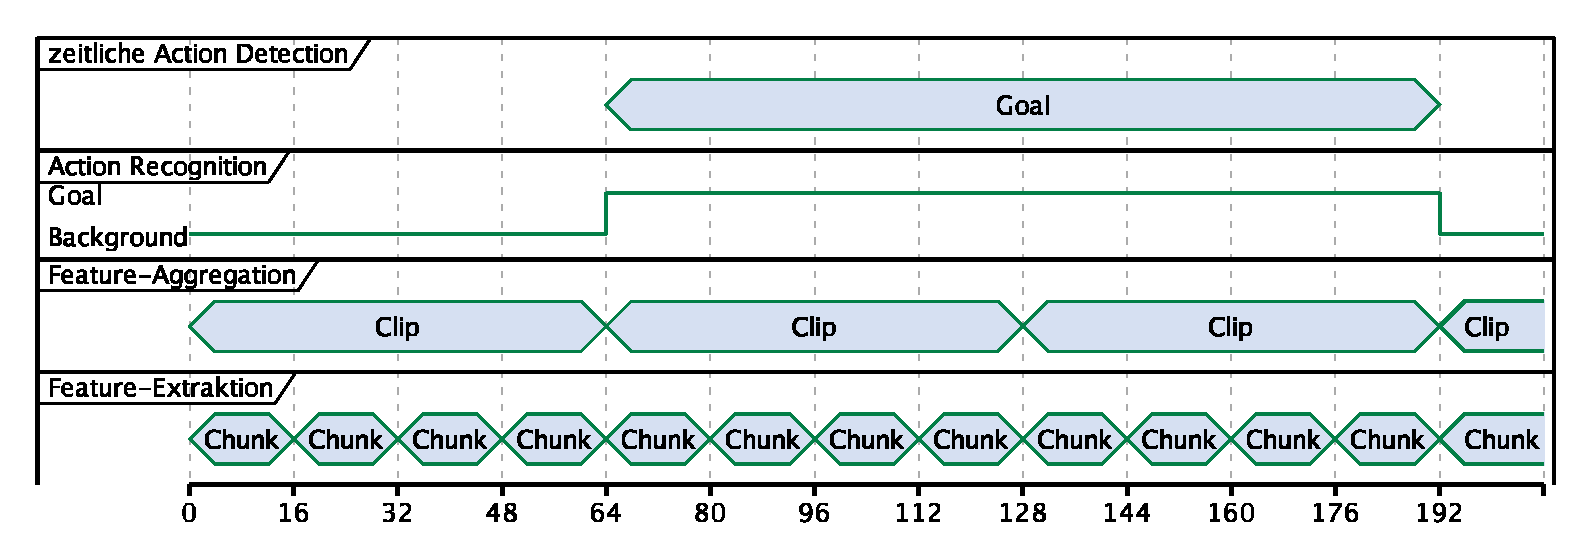
\includegraphics[width=0.9\textwidth, height=0.9\textwidth, keepaspectratio, interpolate]{fig/problems.eps}
    \caption[Teilprobleme im Bereich Video Understanding]{Teilprobleme im Bereich Video Understanding (Quelle: Eigene Darstellung)}
    \label{fig:problems}
\end{figure}

Die Darstellung in \autoref{fig:problems} zeigt eine spezielle (binäre) Form der \gls{har}, die nur zwischen den Zuständen Tor und Nicht-Tor unterscheidet.
Diese binäre Klassifizierung kann zu einer Multi-Class- und zu einer Multi-Label-Variante erweitert werden.
Bei der Multi-Class-Erkennung kann zu jedem Zeitpunkt eine aus $\gls{tld:A}$ Aktionsklassen klassifiziert werden.
Für den Fall, dass sich keine Aktion ereignet, wird ein künstliches Label (oft \emph{Background} genannt) eingeführt.
Im Multi-Label-Fall können sich die Aktionen sogar zeitlich überschneiden, \dh zu jedem Zeitpunkt können $0$ bis $A$ Aktionsklassen erkannt werden.
Die gleichzeitige Erkennung von zwei dicht aufeinanderfolgenden Aktionen innerhalb des gleichen \glspl{clip} ist also nur im Multi-Label-Fall möglich.


\section{Lösungsstrategien}
\label{sec:loesungsstrategien}

Die meisten Ansätze zur Umsetzung einer \gls{har} lassen sich in eine von drei grundlegende Kategorien unterteilen~\cite{Rahmad18, Kothawade19}:

\begin{description}
    \item[Detection \& Tracking]
    Es werden Low-Level-Features erfasst, indem die Akteure (Spieler) in jedem Bild einzeln erfasst und wiedererkannt (getrackt) werden.
    Pro Spieler wird die Differenz zwischen den Bildern (\zB mit Trajektorien oder Optischem Fluss) errechnet, woraus sich ein Bewegungsmuster ergibt.
    Von der Bewegung wird dann auf eine Aktion geschlossen.
    Diese Methode ist allerdings nur bei einer hohen Auflösung einsetzbar und erfordert eine manuelle Anpassung bei abweichenden Daten.
    Ebenso ist die Inferenzzeit vergleichsweise lang.
    Zu den populärsten Methoden gehören \ua \gls{idt}~\cite{Wang13}.
    \item[Feature-Extraktion \& Klassifizierung]
    Bei diesem Ansatz werden Bildinformationen zunächst komprimiert, um die Dimension im Input-Raum zu verkleinern.
    Die \gls{feature}s spezieller Objekte, wie Spielfeldlinien, Spieler oder Spielstandtafel werden einzeln oder als ein globaler Feature-Vektor auf dem Gesamtbild erfasst.
    Bei der anschließenden Klassifizierung werden die Feature-Vektoren mit einem nachgelagertem Klassifizierer (\zB einer \gls{svm}) auf eine Aktionsklasse abgebildet.
    Das Gesamtmodell besteht somit aus mehreren Untermodellen, die jeweils auf verschiedene Aufgaben zugeschnitten sind.
    \item[End-to-end Deep-Learning]
    Diese Ansätze benutzen \glspl{dnn} und bilden alle Zusammenhänge in einem Schritt ab.
    Im Vergleich zu den anderen Ansätzen zeichnet sich Deep-Learning durch seine hohe Zahl von Parametern aus, die optimiert werden müssen.
    Dazu braucht es im gleichen Maße eine hohe Zahl an Beispieldaten.
    Weitere Unterschiede sind eine höhere Rechenlast und damit verbunden eine längere Laufzeit während der Optimierung (\gls{training}).
    Andererseits entfallen bei dieser Methode weite Teile der Vorverarbeitung (Pre-Processing).
    Das Modell erlernt alle Low-Level-Features stattdessen implizit mit~\cite{Rahmad18}.
\end{description}

Vergleicht man die drei genannten Gruppen, so ist nicht nur die Anzahl der Publikationen im Bereich \gls{deep-learning} höher, sondern auch die Genauigkeit der Modelle~\cite{Rahmad18}.
Zudem ist die Umsetzung der beiden übrigen Kategorien aufgrund der aufwendigen Vorverarbeitung wesentlich zeitaufwendiger und würde den Rahmen dieser Arbeit sprengen.
Daher werden im Folgenden ausschließlich \gls{deep-learning}-basierte Ansätze verfolgt.


\section{Neuronale Netze und Deep-Learning}
\label{sec:deep-learning}

\gls{deep-learning}, als Untermenge des Maschinellen Lernens (Machine Learning), setzt auf den Einsatz von Neuronalen Netzen zur Optimierung beliebig komplexer Funktionen.
\glspl{dnn}, die dem menschlichen Gehirn nachempfunden sind, zeichnen sich durch eine Netzwerk-artige Struktur aus, bestehend aus Knoten, die in Schichten angeordnet und miteinander verbunden sind~\cite{Burkov19}.
Das in~\cite{rosenblatt58} erstmals vorgestellte Perceptron (\autoref{fig:dnn} links) ist die einfachste Topologie eines Neuronalen Netzes bestehend aus einem zweischichtigem Netz.
Mit der Hinzunahme weiterer \sog Hidden-Layer zwischen dem Input- und Output-Layer entstehen \emph{tiefe} \glspl{dnn} (auch \gls{mlp}), woher auch der Begriff Deep-Learning stammt~\cite{Burkov19}.
Die in \autoref{fig:dnn} gezeigten grünen Knoten entsprechen sogenannten \fc-Layern (fully-connected), die mit allen Knoten der Vorgänger- und allen Knoten der Nachfolger-Schicht verbunden sind.
Intern können die Layer als Gewichtsmatrizen $W$ repräsentiert werden, die mittels eines Optimierungsverfahren, wie \gls{backpropagation}~\cite{rumelhart86} und anhand von Problem-spezifischer Beispieldaten optimiert werden können.

\begin{figure}
    \centering
    \bigimage{img/02_dnn}{0.4\textwidth}
    \caption{Topologie: \gls{dnn} nach~\cite{Veen17}}
    \label{fig:dnn}
\end{figure}



%Wir betrachten Neuronale Netze als Funktionen $f(x) = y$.
%Das \gls{dnn} erhält einen Input (Reiz) $x$, der über mehrere Schichten entlang der Verbindungen vorwärts propagiert wird und schließlich in einer Senke mündet.
%Jede Schicht wird durch eine Aktivierungsfunktion $\sigma(f_{l_i}) = y_{l_i}$ abgeschlossen, die das Ergebnis in einen bestimmten Wertebereich abbildet.
%Besteht ein Netz aus mehreren Schichten (\gls{layer}) $l_i$, sind diese als Funktionen $f_{l_i}(x) = W_{l_i} * x + b_{l_i}$ definiert, wobei $W$ die jeweilige Gewichtsmatrix und $b$ den Bias-Vektor darstellen.
%Es gilt dann $f(x) = f_{l_L}(\dots(f_{l_2}(f_{l_1}(x))))$ für ein Netz mit $L$ Schichten.
%Ein bestimmter Knoten wird indexiert als $x^{(u_i)}_{l_i}$.
%\autoref{fig:dnn} zeigt zwei mögliche Architekturen topologisch mit zwei \bzw drei Layern.

%\gls{deep-learning} beschreibt den Optimierungsprozess für die Funktion $f$ mit mindestens drei Layern.
%Dabei wird der Fehler für möglichst viele Beispieldaten berechnet und mittels \gls{backpropagation} auf die Gewichte $W_{l_i}$ jedes Layers zurückgeführt.
%So kann der Einfluss jedes Gewichts auf den Fehler bestimmt werden und die Gewichte können einzeln in Proportion zu ihrem Einfluss justiert werden.
%Sofern die Aktivierungsfunktion differenzierbar ist, können alle Parameter innerhalb von $f$ mittels Backpropagation optimiert werden.
%Voraussetzung ist, dass ausreichend viele Beispiele vorhanden sind \cite{Burkov19}.

%Die Aktivierung im letzten Layer ist wiederum abhängig von der Problemstellung \cite{Gugger20}:
%Im Multi-Class-Fall ist die Softmax-Funktion aus \autoref{eq:softmax} weit verbreitet.
%Softmax bildet $y_{i \in \{1, \dots, M\}}$ pro Klasse so ab, dass die Summe Eins ergibt und sich der Classifier für eine der Klassen entscheiden muss.
%Softmax wird in diesem Zusammenhang häufig mit Kreuzentropie (Cross Entropy Loss) als Fehler kombiniert.

%\begin{equation}
%    \label{eq:softmax}
%    softmax(x_i) = \frac{e^{x_i}}{\sum_j e^{x_j}}
%\end{equation}

%Im Multi-Label-Fall funktioniert Softmax nicht, da potenziell mehrere Labelknoten $y_i$ aktiviert werden sollen \cite{Gugger20}.
%In diesem Fall bietet sich, wie auch in der binären Klassifizierung, die Sigmoid-Funktion aus \autoref{eq:sigmoid} an:
%Jeder Knoten wird isoliert betrachtet und der Fehler wird \zB mit binärer Kreuzentropie (Binary Cross Entropy Loss, siehe \autoref{eq:bce}) berechnet:

%\begin{equation}
%    \label{eq:sigmoid}
%    sigmoid(x) = \frac{1}{1 + e^{-x}}
%\end{equation}

%\begin{equation}
%    \label{eq:bce}
%    bce(y, o) = - \sum_{c=1}^A y_{o=c} \log p_{o=c}
%\end{equation}

Abseits von klassischen \glspl{dnn} sind insbesondere die Konzepte von \glspl{cnn} und \glspl{rnn} hervorzuheben.
\glspl{cnn} sind Netze, die häufig im Umgang mit Bildern genutzt werden, da sie besonders gut räumliche Beziehungen abstrahieren können~\cite{Pointer19}.
Hingegen werden \glspl{rnn} für die Verarbeitung sequenzieller Daten und Zeitreihen genutzt~\cite{Pointer19}.
Da Videos sowohl eine räumliche, als auch eine zeitliche Dimension vorweisen, überrascht es nicht, dass Techniken beider Kategorien für die im nachfolgenden Kapitel vorgestellten, aktuellen Lösungsansätze zur \gls{har} relevant sind.
Daher werden die wichtigsten Konzepte und Modelle beider Oberkategorien zum allgemeinen Verständnis der folgenden Kapitel rekapituliert.

\label{sec:conv}

\section{Convolutional Neural Networks}
\label{sec:cnn}

\glspl{cnn} sind Neuronale Netze, die auf die Verarbeitung von Bildern zugeschnitten sind.
Dabei werden lokale (rechteckige) Ausschnitte innerhalb des Bildes mit einem \gls{moving-window}-Ansatz von links nach rechts und von oben nach unten verarbeitet.
Eine Faltungsmatrix (\gls{kernel}), dessen Werte ebenfalls optimierbare Parameter des Gesamtmodells sind, fährt über das Bild und berechnet pro Pixel das innere Produkt des Kernels mit der umliegenden Nachbarschaft des Pixels.
In einem \conv-Layer (in \autoref{fig:cnn} rosa) werden mehrere Kernel initialisiert, um neue Bilder zu erzeugen.
Das Ergebnis jeder Operation ist die Ähnlichkeit zwischen dem Kernel und dem Input-Signal.
Stapelt man mehrere \conv-Layer hintereinander, kann man beobachten, dass in den vorderen Schichten Low-Level-Features, wie Ecken, Kanten und farbliche Übergänge gelernt werden, die in tieferen Schichten zu High-Level-Features, wie geometrischen Formen und Mustern kombiniert werden~\cite{Burkov19}.

\begin{figure}[hb!]
    \centering
    \bigimage{img/02_cnn}{0.4\textwidth}
    \caption{Topologie: \gls{cnn} (Quelle:~\cite{Veen17})}
    \label{fig:cnn}
\end{figure}

Pro Layer ergibt sich eine dreidimensionale \gls{feature-map} aus einem Bild pro Kernel.
Die einzelnen Bilder \bzw die Querschnitte einer Feature-Map werden auch als \glspl{channel} bezeichnet.
Der Input des Netzes besteht typischerweise aus drei Kanälen für den jeweiligen \gls{rgb}-Kanal des Farbbilds.
Eine Faltung, wie sie in tieferen Layern vorkommt (mit mehr als einem Kanal als Input), berechnet immer die Summe aller einzelnen Faltungen~\cite{Burkov19}.

Häufig werden \conv- mit sogenannten \pool-Layern kombiniert (\gls{pooling}), die die Bilder pro Kanal auf eine niedrigerdimensionale Version komprimieren.
In diesen Schichten werden die Informationen in den Feature-Maps weiter komprimiert, allerdings ohne zusätzliche Parameter einzuführen.
Einfache Operatoren, wie der Durchschnitt (Average Pooling) oder das Maximum (Max Pooling) werden auf Teilbereiche der Bilder angewandt.
Dabei werden die Kanäle einzeln verarbeitet und nur die räumliche Dimension wird komprimiert.
Wichtige Hyperparamter für Faltung und Pooling sind zum einen die Dimension des Kernels und die räumliche Schrittweite (Stride) einer Faltung, sowie das Padding~\cite{Burkov19}.

Yann Lecun stellte 1998 die Grundlagen mit seinem LeNet-5 vor~\cite{Lecun98} -- einem \gls{cnn} bestehend aus zwei \conv- und drei \fc-Layern, das Bilder in $S^2=32 \times 32$ Pixeln verarbeiten konnte.
Aufgrund der damalig enormen Rechenlast (zur Optimierung von 60K Parametern) blieb der große Erfolg vorerst aus.
Erst 2012 wurde der Ansatz mit dem Einsatz neuartiger \glspl{gpu} wieder aufgegriffen:
AlexNet~\cite{Krizhevsky12} ist geprägt durch eine tiefere Architektur von 8 Layern und die erstmalige Verwendung vom \gls{relu} als Aktivierungsfunktion (siehe \autoref{eq:relu}) und dem Einsatz Max- statt Avg-Pooling.
Bilder können hier in einer Auflösung von $S^2=224 \times 224$ verarbeitet werden.
Die nächste effizientere Weiterentwicklung war schließlich VGG-16~\cite{Simonyan15}.
Die großen Kernel der vorderen Layer wurden durch die Abfolge mehrerer kleinerer $(3 \times 3)$-Kernel ersetzt, sodass das rezeptive Feld dennoch gleich bleibt (zwei $(3 \times 3)$-Convolutions entsprechen einer $(5 \times 5)$-Convolution).
Zudem ist das Netz mit 16 Layern und 138 Millionen Parametern deutlich tiefer und kann wesentlich mehr Informationen abbilden.

\begin{equation}
    \label{eq:relu}
    relu(x) = \begin{cases}
                    0, & \text{if } x < 0\\
                    x, & \text{else}
    \end{cases}
\end{equation}

\subsection{Inception-Blöcke}
\label{subsec:inception-bloecke}

Eine deutlich schlankere Alternative zu VGG-16 wurde 2014 mit InceptionV1 (auch GoogLeNet)~\cite{Szegedy14} veröffentlicht.
Der Einsatz von sogenannten Inception-Blöcken war der entscheidende Durchbruch.
Inception-Blöcke ersetzen die gewöhnlichen \conv-Layer durch vier parallele Stränge, die am Ende wieder zusammengeführt werden (siehe \autoref{fig:inception}).

\begin{figure}[hb!]
    \centering
    \bigimage{img/02_inception}{0.4\textwidth}
    \caption{Topologie: Inception-Block (Quelle:~\cite{Karim19})}
    \label{fig:inception}
\end{figure}

Jeder Strang beinhaltet eine punktweise Convolution (Pointwise Convolution), wobei mit einem $(1 \times 1)$-Kernel, die Korrelation eines Pixels entlang aller Feature-Maps abbildet und die Anzahl der Feature-Maps dadurch reduziert wird.
Zudem können Filter verschiedener Größe parallel genutzt werden um die Anwesenheit von großen und kleinen Mustern gleichzeitig lokalisieren zu können.
Nach jeder Convolution kommt eine ReLu Aktivierung, die zu einer höheren Nichtlinearität führt~\cite{Pointer19}.

InceptionV1 nutzt nach einem Stamm-Block (\stem-Layer), bestehend aus drei gewöhnlichen \conv-Layern, ausschließlich Inception-Blöcke, sowie zusätzliche \pool-Layer in insgesamt 22 Schichten.
Durch den Einsatz der Inception-Blöcke fällt der Fußabdruck mit rund 5 Millionen Parametern vergleichsweise klein aus.

Eine Erweiterung des Vorgängers mit deutlich größerem Fußabdruck ist InceptionV3~\cite{Szegedy15}.
Dabei wurden die $(3 \times 3)$-Convolutions durch eine effizientere Kombination asymmetrischer $(1 \times 3)$- und $(3 \times 1)$-Convolutions abgelöst.
Auch die größeren Kernel im \stem-Block wurden weiter zerlegt in mehrere $(3 \times 3)$-Convolutions.

In InceptionV4 (2016)~\cite{Szegedy16} wurden noch weitere Inception-Blöcke verwendet, wobei in diesem Modell eine einheitliche Anzahl an Kernels in allen Inception-Blöcken verwendet wird.

\subsection{Residual Learning}
\label{subsec:residual-learning}

Parallel zur Erscheinung von InceptionV1 wurde auch ResNet-50~\cite{He15} und das damit einhergehende Residual Learning vorgestellt.
Residual Learning ist eine Technik zur Vermeidung von Overfitting in Neuronalen Netzen.
Overfitting ist die Folge davon, dass das Netz zu viele Freiheitsgrade hat und so Details der vielen Beispieldaten auswendig lernt, anstatt abstrakte Muster darin zu erkennen.
Dieser Effekt war zuvor bei einem nicht ausgewogenen Verhältnis von Tiefe des Netzes zur Anzahl an Trainingsdatensätzen, unvermeidbar.

\begin{figure}[hb!]
    \centering
    \bigimage{img/02_identity}{0.5\textwidth}
    \caption{Topologie: \res-Block (Quelle:~\cite{Karim19})}
    \label{fig:residual}
\end{figure}

Beim Residual Learning werden gewöhnliche Knoten eines Layers in \res-Layer integriert.
Dabei wird eine zusätzliche Verbindung (Skip Connections) eingeführt, die den Inputs und Output des Layers mithilfe einer punktweisen Multiplikation verknüpft (siehe \autoref{fig:residual}).
Optional wird das eigentliche \conv-Layer von zwei punktweisen $(1 \times 1)$-\conv-Layern umgeben, um die Informationen zusätzlich zu verdichten.
Diese Verdichtungen werden auch als Bottlenecks bezeichnet.
\res-Blöcke werden klassisch in vier \res-Layer (\res1 bis \res4) gegliedert.

Sofern die Möglichkeit des Overfittings besteht, ist das Netz nun in der Lage ein Identitätsmapping (Input $\to$ Input) zu lernen, indem es alle Gewichte eines Blocks auf null setzt.
So können überflüssige Blöcke implizit während des Trainings deaktiviert werden und das Netz kann selbst entscheiden wie viele Layer es benötigt.

Zudem wurde in ResNet-50 erstmalig eine Batch Normalisierung~\cite{Ioffe15} genutzt, was wiederum zu einem schnelleren und stabileren Training führt~\cite{Gugger20}.


Eine alternative Weiterentwicklung zu ResNet ist DenseNet (2018)~\cite{Huang18}, welches zusätzliche Verbindungen zwischen Layern, die nicht direkt aufeinander folgen, herstellt.
Dadurch gibt es zusätzliche Verbindungen und Gewichte.
Im Gegenzug braucht es aber eine deutlich geringere Anzahl an Layern und dünneren Feature-Maps.

In einem sogenannten Dense-Block geht der Input aller vorherigen Feature Maps innerhalb des Blocks ein.
So können Features aus früheren Layern wiederverwendet werden und es müssen weniger zusätzliche (und im gewissen Maße redundanten) Features erzeugt werden.
Im Gegensatz zu ResNet werden die eingehenden Features vergangener Layer allerdings nicht mit punktweiser Multiplikation verknüpft, sondern mit Channel-wise Concatenation, \dh die Input-Features früherer Layer mit den eigentlichen Input-Tensoren konkateniert.
Da die Feature-Maps hierfür jeweils die gleiche Auflösung haben müssen, wird das Netz in mehrere Dense-Blöcke eingeteilt.
Innerhalb der Blöcke wird die Auflösung nicht verändert und alle Layer sind miteinander verbunden.
Zwischen den Dense-Blöcken werden Transition-Layer (\ua mit \pool-Layern) eingebaut, sodass die Auflösung im Hinblick auf die Gesamtarchitektur dennoch reduziert werden kann.

\subsection{Depthwise Separable Convolution}
\label{subsec:group-conv}

Mit Hinblick auf mobile Plattformen war der Einsatz von \gls{cnn} aufgrund zu vieler Rechenoperationen lange nicht denkbar.
Erst durch den Einsatz von Depthwise Separable Convolution in Architekturen, wie Xception (2016)~\cite{Chollet17} oder MobileNet (2017)~\cite{Howard17}, konnte der Einsatz ermöglicht werden.
Das Ziel hierbei war annähernd vergleichbare Ergebnisse bei weniger Parametern und Rechenoperationen zu ermöglichen.

\begin{figure}[h!]
    \centering
    \bigimage{img/02_depth_wise}{0.6\textwidth}
    \caption{Vergleich: Channel-Interaktion in Group Convolution (Quelle:~\cite{Tran19})}
    \label{fig:depthwise}
\end{figure}

Depthwise Separable Convolution bestehen aus Group Convolution und punktweiser Convolution.
Bei einer Group Convolution werden alle Kanäle einer Feature-Map gruppenweise den Kernels der nächsten Schicht zugewiesen.
\autoref{fig:depthwise} zeigt die verschiedenen Formen von Group Convolution:
In \emph{a)} erhält jeder Kernel Zugriff auf jeden Kanal der Feature-Map, sowie es in allen vorherigen \gls{cnn}-Architekturen gängig ist.
\emph{b)} zeigt ein Beispiel, in dem jeder Kernel Zugriff auf zwei Kanäle des Vorgänger-Layers erhält.
Man spricht von Group Convolutions, weil die Zuordnung gruppenweise erfolgt und es keine direkte Interaktion zwischen den Gruppen gibt.
Der Extremfall einer Group Convolution wird in \emph{c)} gezeigt, bei der jede Gruppe aus nur einem Kanal besteht.
In diesem Fall gibt es gar keine direkte Interaktion zwischen den Kanälen.
Da es in \emph{b} und \emph{c} keine direkte Interaktion zwischen Kanälen unterschiedlicher Gruppen gibt, folgt auf die Group Convolution die punktweise Convolution, die alle Kanäle pro Pixel (mit einem $(1 \times 1)$-Filter) kombiniert und die Dimension der neuen Feature-Map reduziert.

\section{Recurrent Neural Networks}
\label{subsec:recurrent-neural-networks}

Die zweite Gruppe relevanter Backbone-Modelle stellen \glspl{rnn} dar.
Dazu zählen Neuronale Netze mit einem internen Zustand, mit dem eine zeitliche Abhängigkeit abgebildet werden kann, ähnlich einem Gedächtnis.
Damit sind sie besonders gut geeignet um sequenzielle Daten mit einer zeitlichen Dimension zu klassifizieren.
Topologisch unterscheiden sie sich durch Zyklen innerhalb des Netzwerks (siehe \autoref{fig:rnn}).

\begin{figure}[h!]
    \centering
    \bigimage{img/02_rnn}{0.2\textwidth}
    \caption{Topologie: \gls{rnn} (Quelle:~\cite{Veen17})}
    \label{fig:rnn}
\end{figure}

In seiner Reinform speichert ein \glspl{rnn} zu jedem Zeitpunkt $t_i$ für den Input $x_{t_i}$ zusätzlich ein Hidden State $h_{t_i}$, der als zusätzlicher Input im nächsten Zeitpunkt $t_{i+1}$ genutzt wird.
Jeder Block hat also eine Rückkopplung zu seinem vorherigen Zustand.
Diese Architektur leidet allerdings besonders am \gls{vanish-gradient}.
Ab einer gewissen Tiefe wird der Einfluss des Fehlers, welcher während der Backpropagation ermittelt wird, verschwindend (vanishingly) gering und das Netz kann im schlimmsten Fall nicht weiter optimiert werden~\cite{Pointer19}.

\subsection*{Long Short-Term Memory (LSTM)}

In der ursprünglichen Form ist es schwer längere zeitliche Zusammenhänge zu erkennen.
Die LSTM-Architektur~\cite{Hochreiter97} erweitert die gewöhnliche \gls{rnn}-Architektur dadurch, dass es die eine explizite Funktion hat, Gelerntes wieder zu vergessen.
Wie viel vergessen wird, ist somit Teil des Trainings, womit es ein längeres Kurzzeitgedächtnis hat als ein reines \gls{rnn}.
Das wird möglich durch den Einsatz verschiedener sogenannter Gates:
Das Input-Gate entscheidet darüber, wie stark der Hidden state (aus dem vorherigen Zeitschritt) in Abhängigkeit von neuem Input geändert wird und der Forget-Gate entscheidet, wie viel alte Information vergessen wird.
Zuletzt entscheidet der Output-Gate darüber welche Informationen an das nächste Layer weitergegeben werden.

\subsection*{Gated Recurrent Units (GRU)}

GRUs~\cite{Cho14} sind eine alternative, schlankere Variante zu LSTMs, wobei Output- und Forget-Gate in eine Einheit (Reset-Gate) überführt werden.
Somit gibt es weniger Parameter und Rechenoperationen.
Auch wenn diese Generation vom RNNs deutlich jünger ist, lässt sich nicht abschließend beurteilen, welche Gruppe die besseren Ergebnisse liefert.


\chapter{Deep-Learning-basierte Action Recognition}
\label{ch:sota}

Dieses Kapitel widmet sich dem aktuellen Forschungsstand im Bereich \gls{har}.
Der Hauptforschungsstrang in diesem Bereich beschäftigt sich mit Modellen, die anhand von generischen Datensets optimiert werden, die ein breiteres Spektrum an Anwendungsdomänen abdecken, als Sportarten, wie Fußball.
So soll sichergestellt werden, dass die Modelle besonders gut abstrahieren und sich in speziellen Domänen (hier Fußball) leicht nachtrainieren lassen (\gls{transfer-learning})~\cite{Burkov19}.
Daher werden im Folgenden Modelle mit allgemeingültiger Anwendbarkeit rekapituliert, die in einem späteren Schritt mit Daten aus der Fußballdomäne weiter abgestimmt werden.
\gls{har} gilt als der Kernproblem aufbauenden Probleme von Action Detection bis Video Understanding~\cite{Jiang19,Xia20}.
Auf diverse Möglichkeiten ungeschnittenen Videos zu verarbeiten oder die \gls{har} in eine zeitliche Action Detection zu integrieren wird gegen Ende des Kapitels eingegangen.

\section{Deep-Learning-Modelle zur Action Recognition}
\label{sec:deep-learning-modelle-zur-action-recognition}

Der Schlüssel zu einer guten \gls{har} ist die Erlernbarkeit von Bewegung (Motion).
Bewegung setzt sich zum einen aus der Erscheinung (appearance) von Objekten innerhalb stiller Frames und zum anderen aus der Dynamik (dynamics) entlang mehrere Frames zusammen~\cite{Sun15,Wang16}.

Die im Nachgang vorgestellten Kategorien haben unterschiedliche Ansätze diese beiden Faktoren zu erlernen und zu kombinieren.
In~\cite{Karpathy14} wurden erstmalig verschiedene Methoden verglichen, Bewegung in Videos einzufangen.
Dabei wurden die in \autoref{fig:fusion-types} gezeigten Ansätze Late-, Early und Slow-Fusion vorgestellt.
Allen drei liegt dasselbe 2D-CNN-Backbone zugrunde, welches einer abgewandelten Form von AlexNet entspricht.

\begin{figure}[h!]
    \centering
    \bigimage{img/03_Karpathy14}{0.8\textwidth}
    \caption[Fusion-Modelle für Frame-Features]{Fusion-Modelle für Frame-Features (Quelle:~\cite{Karpathy14})}
    \label{fig:fusion-types}
\end{figure}

In Late-Fusion-Modellen werden zunächst Features pro Frame erzeugt, wie es in einem 2D-\gls{cnn} der Fall ist und die fertigen Frame-Features werden erst in den allerhintersten Layern verknüpft.
Bei Slow-Fusion-Modellen fließen die Informationen aller Frames hingegen schon im ersten Layer ein.
Ein Kompromiss beider Anätze stellt die Slow Fusion dar, in der Features für je eine Untermenge der Frames verarbeitet und diese hierarchisch verknüpft werden.
Die drei Kategorien werden im weiteren Verlauf als Oberkategorien immer wieder aufgegriffen, während deren konkrete Umsetzung in~\cite{Karpathy14} unter dem Projektnamen DeepVideo referenziert wird.

%\autoref{fig:methods} zeigt einen Auszug konkreter Modelle, die unter diese drei Kategorien fallen und im weiteren Verlauf geneuer vorgestellt werden.

%\begin{figure}[htbp!]
%    \centering
%    \bigimage{fig/methods}{0.9\textwidth}
%    \caption{Lösungsansätze für das \gls{har}-Problem (Quelle: Eigene Darstellung)}
%    \label{fig:methods}
%\end{figure}

\subsection{Early Fusion}
\label{subsec:early-fusion}

Im Early-Fusion-Verfahren aus DeepVideo~\cite{Karpathy14} werden die drei Input-Kanäle (\gls{rgb}) aller Frames konkateniert und gleichwertig in das CNN-Backbone gegeben.
Erscheinung und Dynamik werden also parallel und von Anfang an erfasst.
Allerdings kann das Netz nicht unterscheiden, welche Kanäle zu welchem Frame gehören.
Somit herrscht keine Ordnung unter den Frames, \dh die Reihenfolge geht verloren.
Es kann keine echte Bewegung erkannt werden, sondern nur ein durchschnittliches Erscheinungsbild~\cite{Tran15}.
Das Öffnen einer Tür könnte \zB nicht von dem Schließen einer Tür unterschieden werden.
Ein weiterer Nachteil ist, dass sich mit dieser Methode nur wenige Frames zeitgleich verarbeiten lassen.

Im Slow-Fusion-Verfahren von DeepVideo~\cite{Karpathy14}, das eine hierarchische Form der Early Fusion darstellt, werden zunächst einzelne Frames in überlappende Intervalle gegliedert.
Diese werden dann, wie bei Early Fusion, als gleichwertige Kanäle verarbeitet.
Nach wenigen Schichten werden die Low-Level-Features erneut fusioniert.
Dennoch verliert das Modell die zeitlichen Informationen schließlich nach der letzten Fusion wieder~\cite{Tran15}.

Auch wenn keines dieser Modelle praktische Relevanz erlangte, zeigten die Experimente, dass Bewegung am besten lernbar ist, wenn Erscheinung- und Dynamik im gleichen Tempo erfasst wird.
Das Slow-Fusion-Modell schneidet entsprechend am besten ab.

\subsubsection{Two Stream Network}

Eine weitere Möglichkeit Bewegungsinformationen aus Videos zu extrahieren ist durch die Berechnung von Optischem Fluss.
Die Differenz zweier Bilder kann damit wieder als ein oder zwei (für horizontale und vertikale Bewegungen) neue Bilder gespeichert werden.

Das sogenannte Two Stream Network aus~\cite{Simonyan14} (siehe \autoref{fig:two-stream}) ist ein Modell, das mit zwei Input-Quellen in getrennten Netzen operiert.
Im ersten Stream (Spatial Stream) wird ein einzelner Frame als normales Farbbild in ein CNN-\gls{backbone} gegeben.
Der zweite Stream (Temporal Stream) nimmt mehrere Bewegungsbilder pro \gls{clip}.
Dazu wird für alle Frames des \glspl{clip} vorab die Differenz als Optischer Fluss gespeichert.
Diese Bilder (je zwei pro Ausrichtung) werden als gleichwertige Kanäle in einen zweiten Stream gegeben.
Am Ende werden die Features aus beiden Streams mit einer \gls{svm} fusioniert.

Da die Frames auch hier als gleichwerige Kanäle behandelt werden, zählt es ebenso zu den Early-Fusion-Modellen und leidet daran, das keine Reihenfolgen abgebildet werden kann.
Dennoch erzielt es bessere Ergebnisse, da durch die Hinzunahme von Optischem Fluss externe Dynamik-Features hinzukommen.

Der wesentliche Unterschied zur Early Fusion in~\cite{Karpathy14} ist die getrennte Verarbeitung von Erscheinung und Dynamik in jeweils getrennten Netzen.
Motiviert ist diese Entscheidung durch die Two-Stream-Hypothese aus~\cite{Goodale92}, die besagt, dass der visuelle Kortex des menschlichen Gehirns Bewegung ebenfalls in zwei Strömen erfasst:
dem dorsalen Strom für die Erfassung von Dynamik und dem ventralen Strom für die Erkennung von Objekten.

Trotz langanhaltender Popularität ist der Einsatz von Optischem Fluss in Zusammenspiel mit Deep-Learning problematisch~\cite{Zhu17}:
Zum einen müssen die Differenz-Bilder vorab berechnet werden.
Das führt zu zusätzlichem Zeit- und Speicheraufwand, der mit der Anzahl von Frames skaliert und im Kontext dieser Arbeit nicht unerheblich ist.
Eine Echtzeit-Inferenz längerer \glspl{clip} ist mit gewöhnlicher Server-Hardware schon nicht möglich.
Des Weiteren sind die Modelle nicht Ende-zu-Ende trainierbar.
Die Inferenz besteht aus zwei getrennten Schritten: der Berechnung von Optischem Fluss und dem Training der Netze.
Der Optische Fluss selbst kann als Zwischenergebnis nicht mit-optimiert werden und ist damit nicht unbedingt auf die High-Level-Aufgabe zugeschnitten \cite{Zhu17}.

\begin{figure}
    \centering
    \begin{subfigure}[b]{.5\textwidth}
        \centering
        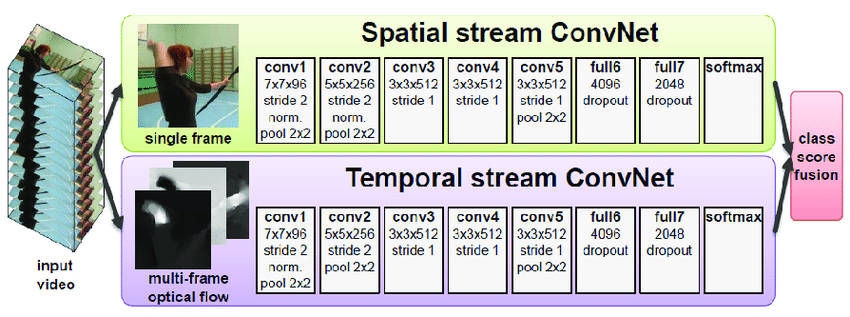
\includegraphics[width=.95\linewidth]{img/03_Simonyan14}
        \caption{Two Stream Network (Quelle:~\cite{Simonyan14})}
        \label{fig:two-stream}
    \end{subfigure}%
    \hfill
    \begin{subfigure}[b]{.5\textwidth}
        \centering
        \bigimage{img/03_Zhu17}{0.95\textwidth}
        \caption{Hidden Two Stream Network (Quelle:~\cite{Zhu17})}
        \label{fig:hidden-two-stream}
    \end{subfigure}
    \caption{Aufbau exemplarischer Early-Fusion-Modelle}
\end{figure}

\subsubsection{Hidden Two Stream Network}

Die genannten Probleme mit Optischem Fluss konnten schließlich mit dem Hidden Two Stream Network aus~\cite{Zhu17} überwunden werden.
\cite{Zhu17} beschreibt einen Ansatz, um beide der genannten Nachteile des Two-Stream-Modells zu kompensieren.
In der Arbeit wurde ein drittes zusätzliches Netz namens MotionNet trainiert, das aus zwei aufeinander folgenden Frames den resultierenden Optischen Fluss selbst generiert.
Das MotionNet wird dem Temporal Stream einfach vorgeschaltet (siehe \autoref{fig:hidden-two-stream}), sodass der Optische Fluss durch die Inferenz des MotionNets direkt errechnet wird und kein aufwendiges Pre-Processing notwendig ist.

Das Ergebnis ist eine bis zu zehnmal schnellere Verarbeitung bei fast gleichbleibender Genauigkeit.
Zudem kann die Erzeugung des Optischen Flusses während des Trainings an die spezielle Aufgabendomäne angepasst und optimiert werden.

\subsection{Late Fusion}
\label{subsec:late-fusion}

In Late-Fusion-Modellen werden die Frames eines \glspl{clip} zunächst nur einzeln in einem 2D-CNN-Backbone zu Frame-Features verarbeitet.
Dies entspricht im ersten Schritt einer Feature-Extraktion, die nur Erscheinungs-Features generiert.
Erst in einem zweiten Schritt wird die Dynamik anhand der Frame-Features erfasst und aggregiert.
Ein entscheidender Nachteil dieser Ansätze ist, dass in den vorderen Layern sehr viele redundante Informationen erhoben werden.
Ein weiterer Nachteil besteht darin, dass dynamische Features im Verhältnis deutlich unterrepräsentiert sind~\cite{Karpathy14}.
Die Feature-Aggregation erfolgt über Konkatenieren, Pooling oder den Einsatz eines \glspl{rnn}.

Die Aggregation in DeepVideo~\cite{Karpathy14} wird durch Konkatenation der Frame-Features gelöst.
Aus den Frames eines \glspl{clip} werden jeweils einzelne Features generiert.
Diese werden alle zu einem langen Vektor konkateniert und abschließend in einem \fc-Layer klassifiziert.
So wird Dynamik durch die Differenz der jeweiligen Frame-Features abgebildet.

\subsubsection{Conv Pooling}

Eine weitere Option Frame-Features zu aggregieren ist durch Pooling.
Dabei werden die Frame-Features vor dem ersten \fc-Layer zu einem 3D-Volume gestapelt und mit einem oder mehreren \pool- und einem \fc-Layer klassifiziert.

In~\cite{Ng15} wurden verschiedene Varianten zur Erfassung von Bewegung getestet.
Die Frame-Features (generiert durch InceptionV1-Backbone) wurden mit einem Max-Pooling-, zwei \fc- und einem Softmax-Layer weiterverarbeitet.
Das Pooling beschränkt sich auf die zeitliche Dimension (Temporal Pooling), sodass die räumliche Dimension komplett erhalten bleibt.
In der zeitlichen Dimension spielt die Reihenfolge allerdings immer noch keine Rolle, da jeweils nur nach Maxima gepoolt wird~\cite{Carreira17}.
Die Klassifikation findet letztlich auf Basis hervorstechender Regionen innerhalb der Frame-Features statt.

%\begin{figure}[h!]
%    \centering
%    \bigimage{img/03_Ng15_conv_pooling}{0.3\textwidth}
%    \caption{Conv Pooling}
%    \label{fig:conv-pooling}
%\end{figure}

Ein technischer Vorteil dieser Architektur ist allerdings, dass sie mit beliebig vielen Frames funktioniert, da das \pool-Layer einen variablen tiefen Input verarbeiten kann.
Das macht das Modell vergleichsweise leichtgewichtig, denn die Zahl der Parameter ist unabhängig von der Zahl der Frames.
Da die Feature-Extraktion viele redundante Informationen für konsekutive Frames berechnet, reicht es in diesem Verfahren aus, die Frames mit einer niedrigere Framerate von 6 \gls{fps} zu samplen.

\subsubsection{Two-Stream-Fusion}

Um den Fortschritt des seinerzeit populären Two-Stream-Modells mit Conv Pooling zu verbinden, stellte~\cite{Feichtenhofer16} 2016 die sogenannte Two Stream Fusion vor.
Das Verfahren unterscheidet sich wesentlich dadurch, dass die Ströme nicht nur am Ende, sondern schon in früheren Layern fusioniert werden.
Im Vergleich zum Conv Pooling wird jedoch kein Temporal Pooling genutzt, sondern ein 3D-Pooling (siehe \autoref{fig:two-stream-fusion}), das sowohl die zeitliche als auch die räumliche Dimension des Frame-Feature-Volumes reduziert.

Die zwei Ströme aus dem Vorgängermodell (spatial-, temporal stream) werden transformiert zu zwei neuen Strömen:
Zunächst findet nach dem fünften \conv-Layer eine Fusion statt.
Als Input werden die Feature-Maps beider Streams abwechselnd zu einer neuen Feature-Map gestapelt und mittels 3D-Faltung gefolgt von 3D-Pooling fusioniert.
Das Ergebnis ist der sogenannte Spatiotemporal Stream, der den alten Spatial Stream ersetzt.
Parallel findet im weiter fortlaufenden Temporal Stream ebenfalls ein 3D-Pooling statt, sodass beide Streams die gleiche Auflösung aufweisen.
Später wird der alter Temporal Stream nach dem letzten \fc-Layer erneut mit dem Spatiotemporal Stream fusioniert.

Die Fusionen bieten erstmalig eine Pixel-weise Kombination beider Streams.
So kann \zB das räumliche Frame-Feature eines erkannten Balls mit dem dynamischen Feature einer Flugkurve pixelgenau kombiniert werden.

Ein Nachteil dieser Architektur ist wiederum, dass Bewegung auf zweierlei Mittel zurückgeführt werden kann.
Durch den Einsatz von Optischem Fluss in mehreren Kanälen und durch die neuartigen Fusion-Layer.
Das Lernen redundanter Informationen kann die Performance so letztlich ausbremsen.

\begin{figure}
    \centering
    \begin{subfigure}[b]{.5\textwidth}
        \centering
        \bigimage{img/03_Feichtenhofer16}{0.95\textwidth}
        \caption{Two Stream Fusion (Quelle:~\cite{Feichtenhofer16})}
        \label{fig:two-stream-fusion}
    \end{subfigure}%
    \hfill
    \begin{subfigure}[b]{.5\textwidth}
        \centering
        \bigimage{img/03_Girdhar17}{0.95\textwidth}
        \caption{ActionVLAD (Quelle:~\cite{Girdhar17})}
        \label{fig:avlad}
    \end{subfigure}
    \caption{Aufbau exemplarischer Late-Fusion-Modelle}
\end{figure}

\subsubsection{Action VLAD}

Ein weiterer Ansatz ist die Klassifikation basierend auf einem Feature-Extraktor wie in~\cite{Girdhar17}.
Das Modell ActionVLAD gilt als eine Erweiterung des Conv Pooling, wobei Features nicht aus dünn gesampleten Frames, sondern aus allen Frames des \glspl{clip} extrahiert werden.
Die Aggregation findet ebenfalls nach dem letzten \conv-Layer eines VGG-16-Backbones statt.

Statt eines Max-Pooling-Layers wird allerdings ein \gls{bovw}-Verfahren ~\cite{Zisserman03} eingesetzt (siehe \autoref{fig:avlad}).
Die aggregierten Features werden auf ein Vokabular von Action Words (in 64 Cluster) projiziert.
Diese Cluster repräsentieren die typischen (Sub-)Aktionen aus denen sich die eigentlichen Klassen herausbilden~\cite{Ghosh18}.
Jeder Frame wird schließlich auf ein Cluster projiziert, sodass sich für den gesamten \gls{clip} ein Feature-Vektor mit je der Anzahl an Treffern pro Cluster ergibt.
Dieser Feature-Vektor wird mithilfe eines weiteren Klassifizierers dann auf die finale Klasse projiziert.
Alle Parameters, darunter die Action Words, sowie die Feature-Extractors werden während des Trainings des eigentlichen Klassifizierers mitgelernt.

Zusätzlich gibt es auch eine Version, die ActionVLAD in die Two Stream Architektur integriert.
Die Features werden hier jedoch wieder separat pro Strom berechnet und erst am Ende kombiniert, in dem der Durchschnitt beider Vektoren genommen wird.

\subsubsection{Feature-Aggregation mit RNNs}

Die dritte Möglichkeit Frame-Features zu aggregieren ist der nachgelagerte Einsatz eines \gls{rnn}.
Die Folge einzelner Frame-Features kann somit als Zeitreihe angesehen werden, die in ihrer ursprünglichen Reihenfolge verarbeitet wird.

In~\cite{Donahue14} wurde erstmalig das Long-term Recurrent Convolutional Networks (LRCN) vorgestellt.
Dort werden je Frame visuelle Features mit einem auf AlexNet basierenden Backbone extrahiert.
Die Frame-Features werden dann nach und nach in ein LSTM-Layer geleitet (siehe \autoref{fig:lrcn}).
Die Klassifizierung eines \glspl{clip} setzt sich schließlich aus dem Durchschnitt aller Outputs $y_{t_i}$ zusammen.

\begin{figure}[h!]
    \centering
    \bigimage{img/03_Donahue14}{0.4\textwidth}
    \caption[Aufbau des LRCNs]{Aufbau des LRCNs (Quelle:~\cite{Donahue14})}
    \label{fig:lrcn}
\end{figure}

Herausfordernd ist hierbei, dass die visuellen Frame-Features genug relevante Informationen für das abschließende LSTM-Layer behalten.
Das Modell wurde jeweils mit RGB-Bildern und Optischem Fluss getestet, wobei die Variante mit Optischem Fluss wesentlich bessere Ergebnisse erzielt.
Dies ist \ua ein Hinweis darauf, dass die Bewegung in den ursprünglichen Bildern erst zu spät erfasst wird.
Das Modell hat ebenfalls eine variable Input-Länge, ist aber deutlich schwerer zu trainieren, da die Backpropagation über alle Frames geschieht und so sehr anfällig für Overfitting ist.

In~\cite{Ng15} wurde neben dem bereits erwähnten Conv Pooling auch ein Modell vorgestellt, das Frame-Features mit einem mehrschichtiges LSTM aggregiert.
Im Gegensatz zum LRCN werden fünf LSTM-Schichten mit je 512 Memory-Zellen statt nur einer Schicht gewählt und das 2D-CNN-Backbone entspricht InceptionV1.
Auch im Training gibt es einen gravierenden Unterschied:
während bei LRCN ein Backpropagation-Schritt pro \gls{clip} (mit $T = 16$ Frames) gemacht wird, wird er in diesem Modell pro Frame (bei $T = 30$) gemacht.

\subsection{3D-CNNs}
\label{subsec:3d-conv}

Die nächste große Generation der \gls{har}-Modelle war die erstmalig in~\cite{Ji13} vorgestellte 3D-Faltung (3D-Convolution).
Die 3D-Faltung funktioniert analog zur 2D-Faltung aus \autoref{sec:cnn}:
Statt eines $(\gls{tld:C} \times S \times S)$-Inputs, erhält das Netz einen $(\gls{tld:C} \times T \times S \times S)$-Input.
Alle \conv- und \pool-Layer haben nun dreidimensionale Kernel und erzeugen vierdimensionale Feature-Maps.

Im Gegensatz zu vorherigen Early-Fusion-Modellen werden zeitliche Informationen nicht gemittelt.
Die zeitliche Ordnung der Frames bleibt also erhalten.
Außerdem werden sie, anders als bei Late Fusion, stets im gleichen Tempo erhoben und kombiniert.
3D-CNNs haben allerdings auch wesentlich mehr Parameter und \gls{flops} als alle zuvor vorgestellten Modelle~\cite{Zhu19}~\cite{Carreira17}.

\subsubsection*{C3D (Convolution 3D)}

C3D~\cite{Tran15} ist das erste 3D-CNN, das an großen \gls{har}-Datensets getestet wurde.
Seinerzeit war es als Feature Extractor konzipiert, der $T=16$ Input-Frames zu einem 4096-Elemente-langen Feature-Vektor komprimiert.
Zur Klassifikation wurde anschließend eine \gls{svm} eingesetzt, wobei auch eine direkte Klassifikation im letzten \fc-Layer möglich ist.
Das Netz basiert auf keinem vorhergegangenen Backbone, hat eine Tiefe von insgesamt 10 Schichten (davon 8 3D-\conv-Layer) und verarbeitet \glspl{clip} mit einer Auflösung von $S=112$ Pixeln.
In jedem Layer wird ein $(3 \times 3 \times 3)$-Kernel, gefolgt von einem $(2 \times 2 \times 2)$-\pool-Layer verwendet.
Entscheidende Vorteile sind eine generische Feature-Extraktion und die kompakte Repräsentation.

Bei seiner Vielzahl an Parametern gestaltet es sich allerdings schwierig das Netz von Grund auf neu zu trainieren.
Ebenfalls problematisch ist die Beschränkung auf $T=16$ Frames.
So muss für längere \glspl{clip} stets der Durchschnitt einzelner Chunks erfasst werden, was mit zusätzlichen Ungenauigkeiten einhergeht.

\begin{figure}[h!]
    \centering
    \bigimage{img/03_Varol16}{0.75\textwidth}
    \caption[Aufbau des LTC-Netzes]{Aufbau des LTC-Netzes (Quelle:~\cite{Varol18})}
    \label{fig:ltc}
\end{figure}

\subsubsection*{LTC (Long-term Temporal Convolution)}

Letzteres Problem sollte durch die Veröffentlichung von LTC~\cite{Varol18} behoben werden.
Das Modell unterstützt mit $T=100$ Frames deutlich längere \glspl{clip}, kompensiert dies aber mit einer deutlich geringeren Auflösung von $S=71$ Pixeln.
Ansonsten ähnelt die Architektur (in \autoref{fig:ltc}) der von C3D mit der Ausnahme, dass ausschließlich $(3 \times 3 \times 3)$-Kernel verwendet wurden.

\subsubsection*{I3D (Inflated 3D ConvNet)}

Mit I3D~\cite{Carreira17} wurde das erste 3D-CNN veröffentlicht, das eine Transfer-Learning-Technik nutzt um bestehende Features eines 2D-CNNs wiederzuverwenden.
I3D basiert auf der Architektur von InceptionV1, die um eine dritte Dimension aufgeblasen (inflated) wird.
Beim Prozess der \emph{Inflation} wird jeder bereits vortrainierte 2D-Kernel um eine dritte Dimension erweitert, indem die vortrainierten Gewichte entlang der zeitlichen Achse kopiert werden.
\Dh das Netz ist danach vortrainiert für die Klassifizierung stiller Videos \bzw Standbilder.

%\begin{figure}[h!]
%    \centering
%    \bigimage{img/03_Carreira17}{0.95\textwidth}
%    \caption{Architektur: I3D (Quelle:~\cite{Carreira17})}
%    \label{fig:i3d}
%\end{figure}

Der Größenunterschied zu C3D und LTC spiegelt sich zwar in der Tiefe des Netzes wider, dennoch hat I3D deutlich weniger Parameter aufgrund der effizienten Inception-Architektur und kann somit deutlich schneller trainiert werden.
\glspl{clip} können mit je $T=64$ Frames inferiert werden.

\subsubsection*{T3D (Temporal 3D)}

T3D~\cite{Diba17} ist analog zu I3D eine 3D-Variante von DenseNet.
Die Besonderheit ist hierbei die Hinzunahme eines neuartigen modularen Block-Typen zur Erfassung dynamischer Features von variabler Dauer.

Bei der gewöhnlichen 3D-Faltung wird stets eine lokale Nachbarschaft des jeweiligen Pixels betrachtet, welches im Mittelpunkt der Faltung steht.
Die hier neuen TTLs (Temporal Transition Layer) erfassen allerdings zeitgleich Bewegungen verschieden langer Zeiträume.
Kurze Bewegungen werden durch einen Kernel mit einer vergleichsweise geringen zeitlichen Dimension (flache Kernel) eingefangen und lange Bewegungen mit einem deutlich tieferen Kernel.
In jedem TTL operieren drei verschiedene Kernel, deren Output zu einer neuen Feature-Map konkateniert und gepoolt wird.
Das Netz kann mit einem flachen Kernel \zB eine kurze Geste des Schiedsrichters einfangen und gleichzeitig mit einem tieferen Kernel den Ball verfolgen, der langsam ins Aus rollt.
Da die räumliche Auflösung innerhalb des TTL stets gleich ist, können die Features pro Kernel anschließend Pixel-genau kombiniert werden.
Die Gesamtarchitektur, sowie die eingesetzten TTLs sind in \autoref{fig:t3d} abgebildet.

\begin{figure}
    \centering
    \begin{subfigure}[b]{.45\textwidth}
        \centering
        \bigimage{img/03_ttl.eps}{\textwidth}
        \caption{Aufbau eines TTLs in T3D (Quelle:~\cite{Diba17})}
        \label{fig:t3d}
    \end{subfigure}%
    \hfill
    \begin{subfigure}[b]{.45\textwidth}
        \centering
        \bigimage{img/03_non-local.eps}{0.95\textwidth}
        \caption{Abbildungen eines NL-Blocks (Quelle:~\cite{Wang18})}
        \label{fig:non-local}
    \end{subfigure}
    \caption{Aufbau von TTLs und Non-Local-Blöcken}
\end{figure}

\subsubsection*{Non-Local Networks}

Die in~\cite{Wang18} vorgestellten Non-Local Networks haben eine ähnliche Absicht, wie die TTLs in T3D.
Analog zu TTLs wurden Non-Local-Blöcke entwickelt, die direkte Verbindungen zwischen entfernten Pixeln abbilden können -- mit dem Unterschied, dass keine zusätzliche Faltung benötigt wird.
Sie transformieren die Feature-Maps eines 3D-CNNs in jedem Pixelwert $i$ wie in \autoref{eq:non-local}:

\begin{equation}
\label{eq:non-local}
\begin{split}
    y_i             & = \sum_{\forall j} f_p(x_i, x_j) g(x_j) \\
    f_p(x_i, x_j)   & = softmax(x_i^T W^T_\theta W_\phi x_j) \\
    g(x)            & = W_g x
%y_i             & = \frac{1}{\sum\limits_{\forall j}f(x_i, x_j)} \sum\limits_{\forall j} f_p(x_i, x_j) W_g x_j \\
%f_p(x_i, x_j)   & = e^{W_{\theta} x_i^T W_{\phi} x_j}
\end{split}
\end{equation}

Die Funktion $f_p$ ist eine paarweise Funktion, die die Ähnlichkeit zweier Pixel ausdrückt und entspricht hier der Embedded-Gaussian-Funktion.
$g(x)$ verknüpft jedes Pixel mit der Gewichtsmatrix $W_g$, die für die jeweilige Aufgabe optimiert werden muss.
$W_\theta$ und $W_\phi$ ergeben sich wiederum aus der punktweisen $(1 \times 1 \times 1)$-Faltung eines Pixels.

Non-Local-Blöcke können nicht-lokale Beziehungen direkt abbilden, indem die Interaktion zwischen allen Pixeln des Input-Volumes berechnet werden (siehe \autoref{fig:non-local}).
Das hat zur Folge, dass insbesondere schnelle Bewegungen besser eingefangen werden können als es durch reine 3D-Faltung möglich ist.
Verglichen mit den verschieden tiefen Filtern in TTLs, müssen hier keine diskreten Grenzen (für die zeitliche Dimension der TTL-Kernel) gezogen werden.
Die Blöcke haben vielmehr die Mächtigkeit Bewegungen jedmöglicher Dauer implizit abzubilden.

Durch den Einsatz eines Non-Local-Blocks bleibt zudem die Größe der Feature-Map erhalten, sodass sie sich an beliebigen Stellen eines 3D-CNNs einfügen lassen.
Die Experimente, in denen Non-Local-Blöcke an verschiedenen Stellen eines I3D-Netzes (NL-I3D) getestet wurden, zeigen, dass schon wenige (\zB 5) Non-Local-Blöcke reichen um genauere Ergebnisse zu erzielen.

\subsubsection*{SlowFast}

Zuletzt wurde in~\cite{Feichtenhofer18} SlowFast vorgestellt -- ein Modell basierend auf einem 3D-ResNet, welches kurze und lange Bewegungen durch eine Architekturänderung separate erfasst und kombiniert.
In SlowFast wird Bewegung durch ein Netz aus zwei Strömen erfasst.
Die beiden Ströme sind wie folgt konzipiert:

\begin{description}
    \item[Slow pathway]
    (langsamer Strang) fokussiert sich auf räumliche Features, indem ein \gls{clip} mit einer niedrigen Framerate gesamplet wird.
    Aufgrund der niedrigen Framerate können nur wenig redundante Informationen gesammelt werden.
    Dies wird zusätzlich gehemmt, indem die Hälfte der Residual-Blöcke nur mit 2D-Faltungen operieren.
    \item[Fast pathway]
    (schneller Strang) generiert räumliche Features, indem ein \gls{clip} mit einer höheren Framerate gesamplet wird und wenige Kanäle zur Verfügung stehen.
    So wird ihm die Möglichkeit genommen sich räumliches zu fokussieren.
    Stattdessen muss er sich implizit auf die Dynamik zwischen den Frames fokussieren.
\end{description}

\begin{figure}[h!]
    \centering
    \bigimage{img/03_Feichtenhofer18}{0.8\textwidth}
    \caption[Aufbau des SlowFast-CNNs]{Aufbau des SlowFast-CNNs (Quelle:~\cite{Feichtenhofer18})}
    \label{fig:slowfast}
\end{figure}

An zwei Stellen im Netz werden die dynamischen Features vom schnellen Strang in den langsamen Strang fusioniert.
Diese Verbindungen werden als Lateral Connection bezeichnet und ähneln dem Vorgehen in der 3D-Fusion~\cite{Feichtenhofer16}.
Schließlich werden die Features beider Stränge je mit einem Avg-\pool-Layer auf eine fixe Länge gestaucht und konkateniert.
Ein abschließendes \fc-Layer dient zur Klassifikation.
Die Gesamtarchitektur ist in \autoref{fig:slowfast} zu sehen.

Das Vorgehen ist motiviert durch die Funktionsweise Retinaler Ganglienzelle im menschlichen Auge.
Dort operieren P-Zellen (\emph{P} für parvozellulär) mit einer geringeren Frequenz als M-Zellen (\emph{M} für magnozellulär).
Das Verhältnis von P- und M-Zellen ist etwa 4:1.
Genau dieses Verhältnis wurde auch in der Architektur abgebildet, indem der Slow Pathway 80 \% aller Parameter beansprucht.

Durch das dynamische Avg-Pooling am Ende ist die Summe aller Parameter unabhängig von der \gls{clip}-Länge (nicht aber die Größe der Feature-Map).
Es ist derart implementiert, dass die \conv-Features auf eine fix definierte Zielauflösung komprimiert werden, sodass theoretisch ein Training mit beliebig hoher Auflösung $T \times S \times S$ möglich ist.

Ein entscheidender Hyperparameter ist die Wahl von $\alpha$, der das Verhältnis der Frameraten in Slow- und Fast-Pathway angibt.
\Dh der Fast Pathway erhält $\alpha$-mal so viele Frames als Input, wie der Slow Pathway.
Das Verhältnis verfügbarer Kanäle pro Pathway ist hingegen immer konstant bei $8:1$.
Getestet wurden verschiedene Varianten mit $\alpha = 8$ und $\alpha = 4$, basierend auf ResNet-50 und ResNet-101, sowie unter optionaler Hinzunahme von Non-Local-Blöcken.

\subsection{Faktorisierte 3D-CNNs}
\label{subsec:factorized-convolution}

Spätestens mit der Veröffentlichung von I3D galt 3D-Faltung als der neue State of the art.
Aufgrund der Vielzahl an Parametern waren diese Modelle allerdings noch immer für viele Bereiche zu groß und zu schwer zu trainieren.
Infolgedessen wurden viele Ansätze publiziert, die versuchen die Idee von dreidimensionaler Faltung zu approximieren und dabei annähernd gute Ergebnisse mit weniger Parametern und Rechenoperationen zu ermöglichen.
Man spricht in diesem Zusammenhang von einer Faktorisierung der gewöhnlichen 3D-Faltung, die durch Architekturänderungen, die Einführung neuartiger Block-Typen oder durch die Anwendung separierbarer Faltung erfolgt.

\subsubsection{Faktorisierte Architektur}

In~\cite{Sun15} wird mit FstCN (Factorized spatio-temporal convolutional network) versucht 3D-Faltung in räumliche 2D-Faltung gefolgt von einer 2D-Faltung über die Zeit- und Kanaldimension, zu ersetzen.
Die Frames werden zunächst einzeln verarbeitet, sodass man ${T}$ 3D-Feature-Maps $(\gls{tld:C} \times S \times S)$ erhält.
Nach der normalen 2D-Faltung wird ein 4D-Tensor $(T \times \gls{tld:C} \times S \times S)$ aus allen Feature-Maps generiert und so transformiert, dass eine Feature-Map $(S^2 \times T \times C)$ entsteht.
Es entsteht also ein Volume, welches in seinem Querschnitt ein Bild pro Pixel enthält.
Die Pixelwerte ergeben sich aus dem jeweiligen Kanal der Feature-Map und dem Frame-Index.
Diese Bilder werden nun analog mit 2D-Faltung weiter verarbeitet.

Zu beachten ist, dass die komplette Architektur durch Matrixtransformationen und 2D-Faltung faktorisiert wird.
Dieser Teil findet allerdings erst in den hinteren Layern des Netzes statt, womit es weiter zu den Late Fusion Modellen zählt.
Die Architektur hat zudem den Nachteil, dass Bewegungen nur über den gesamten Zeitkontext des \glspl{clip} erfasst werden können.
Kurze Bewegung oder Kombinationen von kurzen Bewegungen sind somit schwieriger abzubilden.

\subsubsection{(2+1)D-Faltung}

Statt 3D-Faltung einmalig durch eine globale Architekturänderung zu faktorisieren, wurden in späteren Publikationen Ansätze entwickelt, die die 3D-Faltung in mehrere Zwischenoperationen faktorisieren und diese als neuen Blocktyp an zahlreichen Stellen in der Gesamtarchitektur einbinden.

Das erste relevante Modell dieser Kategorie ist P3D~\cite{Qiu17}, deren Grundlage ein 3D-ResNet-Backbone ist.
In dem Netz wird jeder einzelne \res-Block faktorisiert, indem die bestehenden 3D-Kernel $(T \times S_x \times S_y)$ durch die Abfolge eines räumlichen $(1 \times S_x \times S_y)$- und eines zeitlichen $(T \times 1 \times 1)$-Kernels ersetzt wird.
Das Netz erfasst somit iterativ im Wechsel erst räumliche und dann zeitliche Features.

Weiter werden drei der in \autoref{fig:p3d} gezeigten Blocktypen eingeführt und jeder bestehende \res-Block wird durch die Abfolge aller drei Blocktypen hintereinander ersetzt.

\begin{figure}[h!]
    \centering
    \bigimage{img/03_Qiu17}{0.45\textwidth}
    \caption[Kombination von P3D-Blöcken]{Kombination von P3D-Blöcken (Quelle:~\cite{Qiu17})}
    \label{fig:p3d}
\end{figure}

P3D ist nicht nur deutliche schlanker als vorherige 3D-CNNs.
Durch die Einführung zusätzlicher ReLu-Aktivierungen zwischen den 2D- und 1D-\conv-Layern entsteht auch doppelt so viel Nichtlinearität als zuvor.
Das Netz ist damit deutlich einfacher zu optimieren und kann komplexere Funktionen abbilden~\cite{Tran18}.

In~\cite{Tran18} wurden die Erfolge von P3D erneut aufgegriffen und im Zuge des Modells R2+1D verbessert.
Auch hier werden die \res-Blöcke jeweils durch 2D- gefolgt von 1D-\conv-Layern ersetzt.
Im Vordergrund steht hierbei allerdings die direkte Vergleichbarkeit mit 3D-Faltung indem, verglichen mit einem 3D-ResNet, die gleiche Zahl an Parametern verwendet wird.

Topologisch unterscheidet sich R2+1D von P3D durch den konsequenten Einsatz eines \res-Blocktypen, der dem Typ A aus \autoref{fig:p3d} entspricht.
Zusätzlich werden keine Bottlenecks verwendet und das Netz kann dank eines dynamischen Avg-\pool-Layers (analog zu dem in SlowFast) mit einer variablen Input-Länge aufgerufen werden.

\subsubsection{Separierbare Faltung}

Die in \autoref{subsec:group-conv} bereits vorgestellte separierbare Faltung stellt ebenfalls eine Form von Faktorisierung im Sinne der Kanal-Interaktion dar.
In~\cite{Tran19} wurden CSNs (Channel-Separated Convolutional Networks) vorgestellt.
CSNs basieren ebenfalls auf einem 3D-ResNet, benutzen jedoch separierbare Faltung.
Für eine 4-dimensionale Feature-Map, ersetzt die Faktorisierung nun die normale 3D-Faltung durch eine punktweise Faltung mit $(1, 1, 1)$-Kernel über alle Feature-Maps und eine separierbare Faltung mit $(3, 3, 3)$-Kernel pro Kanal.
Erstere sorgt für Interaktion zwischen den Kanälen innerhalb eines Pixels.
Letztere berechnet für einen einzelnen Index der Feature-Map die zeit-räumlichen Features.

Präsentiert wurden in diesem Zuge zwei verschiedene Modelle:
\begin{description}
    \item[interaction-preserved (ip-CSN)] Die \conv-Layer werden durch punktweise Faltung, gefolgt von Depthwise Convolution ersetzt.
    \item[interaction-reduced (ir-CSN)]  Die \conv-Layer werden nur durch Depthwise Convolution ersetzt.
    Alleine durch die Bottleneck-Blöcke der ResNet-Architektur kann noch Kanal-Interaktion hergestellt werden.
\end{description}

Ein noch globalerer Ansatz wird in~\cite{Feichtenhofer20} mit X3D (Expand 3D) präsentiert.
Grundlage ist eine 2D-Variante des Slow Pathway aus SlowFast, der ebenfalls separierbare Faltung, wie in ip-CSN, nutzt.
Die Basisarchitektur wird auf Basis verschiedener Faktoren schrittweise in eine dreidimensionale Variante expandiert:
Neben der raum-zeitlichen Dimension, wird auch die Dichte der gesampleten Frames (Framerate), die Anzahl der Kanäle innerhalb der Layer und die Anzahl der Layer selbst variiert.
Folgende Faktoren (siehe~\autoref{fig:x3d}) wurden mithilfe eines Coordinate Descent Algorithmus~\cite{Wright15} optimiert, um die finale Architektur zu bestimmen:

\begin{description}
    \item[$\gamma_s$] Faktor für höhere Auflösung ($\gamma_s = 1$ entspricht 112 Pixeln)
    \item[$\gamma_t$] Faktor für zusätzliche Frames ($\gamma_t = 1$ entspricht einem einzelnen Frame)
    \item[$\gamma_\tau$] Faktor für Subsampling: Nur jeder $\gamma_\tau$-te Frame wird gesamplet. ($\gamma_\tau = 1$ entspricht der Original-Framerate)
    \item[$\gamma_w$] Faktor für zusätzliche Residual-Blöcke innerhalb der vier \res-Layer der ResNet-Architektur ($\gamma_d = 1$ entspricht 1, 2, 5 und 3 Blöcken).
    \item[$\gamma_w$] Faktor für zusätzliche Kanäle pro Layer
    \item[$\gamma_b$] Faktor für zusätzliche Kanäle -- exklusiv für Bottleneck-Layer innerhalb der \res-Blöcke
\end{description}

\begin{figure}[h!]
    \centering
    \bigimage{img/03_Feichtenhofer20}{0.75\textwidth}
    \caption[Expansionsfaktoren in X3D]{Expansionsfaktoren in X3D (Quelle:~\cite{Feichtenhofer20})}
    \label{fig:x3d}
\end{figure}

In mehreren Phasen wurden die einzelnen Parameter jeweils um einen maximalen Faktor vergrößert.
Die Maximalwerte ergeben sich aus der in \gls{flops} gemessenen Komplexität der Gesamt-Architektur, die pro Phase durch das Doppelte der vorherigen Phase gedeckelt wird.
Für jeden Parameter wird die Änderungen durch den jeweils maximierten Faktor getestet und der beste Faktor wird in die nächste Phase übernommen.
Dieser Prozess wurde insgesamt 13 mal wiederholt, wodurch sechs Versionen (X3D-XS bis X3D-XXL) der Architektur entstanden -- darunter:

\begin{description}
    \item[X3D-S] Alle Parameter bis auf $\gamma_w$ wurden in den ersten 7 Iterationen erhöht ($\gamma_t$ und $\gamma_\tau$ davon zweimal).
    Das Modell samplet $T=13$ mal jeden sechsten Frame ($\tau = 6$) bei einer Auflösung von $S=160$ Pixeln.
    \item[X3D-XL] Nach der zehnten Iteration steht ein Modell mit $T=16$, $\tau = 5$ und $S=312$.
\end{description}

Die Ergebnisse zeigen zum einen, dass mehrere Sekunden langes Videomaterial auch mit wenigen Frames und einem dünnen Sampling verarbeitet werden kann.
Zum anderen sind besonders die Modelle (M bis XXL) interessant, da sie eine deutlich höhere Auflösung $S$ in Kombination mit deutlich weniger Kanälen als vorherige Modelle aufweisen und dabei zum Teil auch bessere Ergebnisse erzielen.
Vor allem aber sticht die geringe Zahl an Parametern hervor, die mit keiner der vorherigen Faktorisierungsmethoden vergleichbar ist.

\section{Long-term Aggregation Frameworks}
\label{sec:long-term-aggregation-frameworks}

Die meisten der vorgestellten Modelle können nur \glspl{clip} einer fixen oder zumindest begrenzten Länge $T$ klassifizieren.
Dieser Rahmen liegt je nach Modell zwischen 16 und 64 Frames.

Einige Modelle (darunter R2+1D, CSN, SlowFast und X3D) ermöglichen durch den Einsatz eines dynamischen Avg-\pool-Layers eine Variable Input-Länge.
Allerdings ist die Nutzung nur dann optimal, wenn die Modelle zuvor auch mit der gleichen Anzahl an Frames trainiert wurden.
Problematisch ist auch, dass die Feature-Maps trotzdem proportional zu $T$ mitwachsen, sodass diese Möglichkeit in der Praxis \zB durch das Speicherlimit einer GPU limitiert wird.

Eine weitere Möglichkeit, die aber ebenfalls nur im geringen Maße praktikabel ist, ist die Erhöhung des Zeitschritts $\tau$ \cite{Ng15}.
Einige Modelle, wie SlowFast oder X3D, nutzen ohnehin nicht jeden Frame eines Clips.
Werden die Frames allerdings mit einem zu hohen Zeitschritt gesamplet, kann insbesondere bei 3D-\glspl{cnn} die Performance einbrechen, da konsekutive Frames zu unterschiedlich sind und die Kernel weniger Zusammenhänge herstellen können.

Benötigt der Klassifizierer einen deutlich längeren Zeitkontext $\Delta$, als das trainierte Modell abbilden kann, sind weder das dynamische Avg-Pooling noch Subsampling ausreichend.
Stattdessen kann auf spezielle Long-term Aggregation Frameworks zurückgegriffen werden.

\subsubsection*{TSN (Temporal Segments Network)}

Ein besonders populäres Framework ist das TSN~\cite{Wang16}~\cite{Wang19}.
Es bettet das eigentliche \gls{har}-Modell in einen spezielles Trainingssetup (siehe \autoref{fig:tsn}) ein.
TSN unterteilt den \gls{clip} zunächst in Unter-Segmente (Snippets).
Innerhalb dieser Snippets wird jeweils zufallsbasiert ein Intervall bestimmt, dessen Länge $T$ in das entsprechend vortrainierte \gls{har}-Modell passt.
Diese Snippets werden vom HAR-Modell inferiert, sodass man die Scores des letzten \fc-Layers als Output erhält.
Für jeden Output-Vektor wird der Fehler pro Klasse berechnet und über die Snippets gemittelt.
Darüber wird abschließend die Aktivierung berechnet, die zur Klassifizierung dient.

Die Architektur ist differenzierbar und wird optimiert mit dem über alle Segmente aggregiertem Output.
Somit können die Modellparameter anhand mehrere Snippets optimiert werden.
In der ursprünglichen Form wurde TSN mit dem Two Stream Modell genutzt.
Technisch gesehen lässt sich allerdings jedes der genannten Modelle einbinden~\cite{Kothawade19}.

\begin{figure}[h!]
    \centering
    \bigimage{img/03_Wang19}{0.8\textwidth}
    \caption[Aufbau des TSNs]{Aufbau des TSNs (Quelle:~\cite{Wang19})}
    \label{fig:tsn}
\end{figure}

\subsubsection*{FASTER (Feature Aggregation for Spatio-temporal Redundancy)}

Alternativ zu TSN kann das jeweilige \gls{har}-Backbone durch ein- oder mehrere \gls{rnn}-Layer erweitert werden.
Exemplarisch wird hier FASTER~\cite{Zhu19} erwähnt.
Durch FASTER soll nicht nur eine zeitliche Struktur über einen längeren Kontext abgebildet werden.
Zusätzlich soll vermieden werden, dass redundante Informationen erhoben werden.

Die Features des letzten \conv-Layers des CNN werden durch ein Avg-\pool-Layer geleitet.
Diese Features werden dann als Input einer GRU verarbeitet und haben Einfluss auf deren Hidden State.
Um das Modell zu beschleunigen können statt eines Backbone-Modells zwei verschiedene Versionen verwendet werden, wobei beide vom gleichen Typ, aber unterschiedlicher Tiefe sein sollten (\zB R2+1D-34 und R2+1D-152).
Das tiefere der beiden Backbones soll mehr Details erfassen und Aktionen sicher vorhersage, während das flachere sich auf Änderungen innerhalb einer Szene beschränkt.

\section{Zeitliche Action Detection}
\label{sec:temporal-action-detection}

Zuletzt soll ein kurzer Einblick zur Umsetzung einer zeitlichen Action Detection gegeben werden.
Da diese Arbeit den Fokus auf eine \gls{har} legt, werden die Konzepte nur oberflächlich angerissen.

Im Allgemeinen können drei Kategorien unterschieden werden~\cite{Buch17}:
Eine zweischrittige Verarbeitung aus \gls{har}-Klassifizierer und nachgelagerter Intervallgenerierung, eine zweischrittige Verarbeitung aus vorgelagerter Generierung von Intervallen und der anschließenden Klassifizierung pro Segment, sowie der Ende-zu-Ende-Verarbeitung in einem Netz.

Die erste Gruppe entspricht einem naiven Ansatz, indem die Videos mit einem bestimmten Versatz, der Einfluss darauf hat, wie stark sich die \glspl{clip} überschneiden, segmentiert werden.
Dabei wird jeder \gls{clip} mit einem \gls{har}-Backbone entlang der Zeitachse klassifiziert.
Die Klassifizierung des Backbones bezieht sich dann jeweils auf den Mittelpunkt des \glspl{clip}.
Aus diesen Klassifizierungsscores können im Nachgang nun Intervalle für jede Klasse abgeleitet werden.

Die zweite Gruppe ist geprägt durch Modelle, wie BSM (Boundary-Sensitive Network)~\cite{Lin18} und BMN (Boundary-Matching Network)~\cite{Lin19}, die im ersten Schritt Intervallvorschläge (Proposals) für potenzielle Aktionen liefert, ohne direkt zu wissen, um welche Art von Aktion es sich handelt.
Die Vorschläge werden also für alle Klassen auf die gleiche Art und Weise erhoben.
Anschließend können \glspl{clip} für jedes Proposal generiert werden und mit dem \gls{har}-Backbone klassifiziert werden.
Praktisch an diesem Vorgehen ist, dass schon im ersten Schritt Segmente ohne Aktionen ausgeschlossen werden, wodurch ein Großteil des ursprünglichen Videos gar nicht mehr vom Backbone klassifiziert werden muss.
Negativ ist der Punkt, dass die Generierung der Proposals nicht zwingend auf die Endaufgabe zugeschnitten ist (es sei denn beide Netze werden Ende-zu-Ende trainiert) und dass Frames in beiden Stufen separate geladen und verarbeitet werden.

Zur dritten Gruppe gehört \ua SS-TAD (Single-Stream Temporal Action Detection)~\cite{Buch17}.
Die grundlegende Idee ist, sich zu merken, wann eine Aktion anfängt und aktiv zu erkennen, wann sie aufhört.
Dazu wird das Video in \glspl{clip} von $T=16$ Frames segmentiert, die mit einem 3D-CNN zu visuellen Features enkodiert werden.
Die Scores pro Klasse werden in ein Modell, bestehend aus zwei \gls{rnn}-Modulen für Proposal Generation und Klassifizierung, gegeben.
Die Proposals ergeben sich aus der Aktivierung eines $T$-elementigen Outputs, wobei jeder Index für die Anzahl vergangener Frames steht, die die aktuelle Aktion bereits überdauern.

\section{Datensets und Benchmarks}
\label{sec:datensets-und-benchmarks}

Der Sportsektor zählt zu den besonders anspruchsvollen Domänen im Bereich \gls{har}~\cite{Sozykin17}.
Dennoch können durch Techniken des Transfer-Learnings, bestehende Low-Level-Features, auf die hier betrachtete Aufgabe übertragen werden -- selbst wenn diese mithilfe generischer Datensets aus übergreifenden Domänen generiert wurden.
Da bisher kein Datenset existiert, das Spielaktionen im gesuchten Umfang bereitstellt, müssen neue Daten erhoben werden, die sich an den Best Practices bestehender Datensets orientieren.
Dazu werden die gängigen Datensets im Bereich \gls{har} kurz vorgestellt und in \autoref{tab:dataset} verglichen:

\begin{description}
    \item[UCF101]~\cite{Soomro12} Einfaches \gls{har}-Datenset mit ungeschnittenen Videos und einfachen Labels aus 101 Klassen (davon 25 aus dem Sportbereich).
    Die Videos sind hierarchisch nach Labeln in Ordnern sortiert.
    \item[THUMOS14]~\cite{THUMOS14} Erweitert einen Teil aus UCF101 um Intervallmarkierungen zur zeitlichen Action Detection.
    Betroffen sind 21 der 101 Klassen.
    Die \gls{annotationen} werden in Textdateien pro Klasse gespeichert.
    Jeder Eintrag besteht aus dem Videonamen, Start- und Endpunkt der Aktion.
    \item[Sports1M]~\cite{Karpathy14} Auto-Generiertes Datenset aus 1 Mio YouTube Videos zu Sportaktionen.
    \item[ActivityNet]~\cite{Caba15} Datenset zur zeitlichen Action Detection, beinhaltet 200 Klassen zu 20,000 Videos.
    Die Markierungen werden strukturiert in einer JSON-Datei gespeichert.
    \item[Kinetics-400]~\cite{Kay17} Manuell annotiertes Datenset aus 650,000 \glspl{clip} und 400 Klassen.
    Erweiterung mit 600 und 700 Klassen existieren ebenfalls.
\end{description}

\subsubsection*{Fußball-Datensets}

Im Bereich Fußball wurden mit SoccAct-4~\cite{Ballan09} und SSID~\cite{Jiang16} erstmalig Datensets veröffentlicht, die im Kontext von Deep-Learning aufgrund ihrer Größe jedoch keine Relevanz erreichten.
Erst mit SoccerNet~\cite{Giancola18} wird ein großspuriges Datenset für Fußball-Aktionen erzeugt.
Die Aktionen beschränken sich auf Tore, Karten und Auswechslungen, die sekundengenau innerhalb eines Spiels erhoben wurden.
Die \gls{annotationen}, der Code und auch die zugehörigen Videos aus sechs europäischen Fußballligen sind der Öffentlichkeit zugänglich.

Eine Erweiterung von SoccerNet stellt SoccerDB~\cite{Jiang19} dar, welches sich in großen Teilen mit SoccerNet überschneidet.
Statt drei, werden hier jedoch 10 Klassen annotiert, die sich in vielen Fällen überschneiden, was es zu einem Multi-Label-Datenset macht.
Außerdem wird zusätzliches Videomaterial aus asiatischen Fußballligen verwendet.

\begin{table}
    \centering
    \small
    \csvreader[no head,tabular=|l|r|r|r|,
    table head=\hline,late after line=\\\hline]{tbl/datasets.csv}
    {1=\colDataset,2=\colVideos,3=\colClasses,4=\colDuration}
    {\colDataset & \colVideos & \colClasses & \colDuration}
    \caption[Vergleich bestehender Datensets]{Vergleich bestehender Datensets}
    \label{tab:dataset}
\end{table}

Das Baseline-Modell in SoccerNet segmentiert vorab die ungekürzten Videos in 60-Sekunden-\glspl{clip}.
Jeder \gls{clip} wird mit den Aktionen, die innerhalb des \glspl{clip} stattfinden, gelabelt.
Bei den meisten \glspl{clip} findet jedoch keine der genannten Aktionen statt.
Diese werden als \emph{Background} gelabelt.

Die eigentliche Verarbeitung besteht aus einem mehrstufiges Modell aus folgenden drei Zwischenschritten:

\begin{enumerate}
    \item Feature-Extraktion mit 2D-ResNet für Frames alle 0.5 sek
    \item Konkatenation der Features und \gls{pca} zur Komprimierung auf 120 Einträge
    \item Klassifizierung der komprimierten Features mit ActionVLAD
\end{enumerate}

Das Ergebnis ist eine \gls{map} von 67,8 \%.
Zu beachten ist, dass mit \gls{map} der Durchschnitt der Precision von nur drei der insgesamt vier Klassen gemeint ist.
Die Precision der \emph{Background}-Klasse wird explizit herausgerechnet.

Als Baseline für SoccerDB wurde ein SlowFast-50 Modell verwendet, das eine \gls{map} von 69,24 \% erreicht.
Zum aktuellen Stand\footnote{Stand: 01.09.2020} ist dieses Datenset allerdings noch unveröffentlicht.

\chapter{Konzeption}
\label{ch:concept}

\begin{tcolorbox}[title=Todo]
    \begin{itemize}
        \item TSN: Argumentation schlüssig?
        \item Max oder Avg bei TestSet-Inferenz
    \end{itemize}
\end{tcolorbox}

In diesem Kapitel werden die Schritte und Entscheidungen erläutert, die zur Erhebung der Daten, zum Training des Classifiers und für die spätere Anwendung notwendig sind.
Dazu werden vorab einige Entscheidungen und Anforderung an die zu entwickelnden Module geknüpft.

\section{Zwischenschritte}
\label{sec:steps}

Der Prozess bis zur fertigen Inbetriebnahme schließt folgende drei Schritte ein, die in dieser Reihenfolge abgeschlossen werden müssen:

\begin{description}
    \item[Data Engineering] Die Daten müssen erhoben und mit dem Deep Learning Modell in Einklang gebracht werden.
    Aus rohen Videos und strukturierten Annotationen werden Samples in ein einheitliches \gls{ml}-Datenset überführt.
    \item[Training] Es muss ein einheitlicher Trainingsablauf definiert werden, um die Ergebnisse einzelner Experimente vergleichen zu können.
    Dabei werden Metriken zur Beurteilung der Modelle und zur Analyse von Konflikten erhoben.
    \item[Integration] Der trainierte Action Classifier muss in eine Temporal Action Detection integriert werden, sodass ungeschnittene Videos ganzer Spiele verarbeitet werden können.
    Schließlich muss der Classifier in eine Nutzerschnittstelle integriert und bereitgestellt werden.
    Die Integration soll zwar ermöglicht werden ist allerdings nicht im Rahmen dieser Arbeit inbegriffen.
\end{description}

\section{Datenquellen}
\label{sec:datenquellen}

Essenziell für das Data-Engineering ist, dass die Trainingsdaten die richtigen Informationen enthalten, die es dem Modell erst ermöglichen notwendige Zusammenhänge zu abstrahieren.
Die Daten müssen genug Informationen enthalten, um die Spielaktion lernbar zu machen.
Zudem sollten die Daten ein möglichst diverses Spektrum und einen geringen Bias (siehe \cite{Gugger20}) aufweisen und keine Ausrichtung auf spezielle Eigenschaften haben.
Aus den genannten Gründen wird sich dagegen entschieden nur Aufnahmen einer Taktischen Kamera oder eines bestimmten Stadions zu verwenden.
Damit das \gls{har}-Modell ausreichend gut adaptiert werden kann, wird stattdessen der Versuch unternommen ein Datenset zu generieren, das Spiele verschiedener Mannschaften, Nationalitäten und Geschlechter beinhaltet.
Zudem soll das Videomaterial verschiedenen (TV-)Quellen zugrunde liegen, sodass sich das Modell nicht auf bestimmte Eigenschaften des Kameraschnitts (wie Art der Kameraführung, Wiederholungen, Einblendungen, Bildqualität) einschießt.

Diese Rohdaten werden anschließend in ein \gls{ml}-Datenset konvertiert.
Neuronale Netze lernen mit Samples $(X, Y)$, wobei $x \in X$ ein vierdimensionaler Video-Tensor und $y \in Y$ das Output-Label ist.
Alle Samples $x$ entsprechen multidimensionalen Matrizen (Tensoren) der Größe $x \in R^{C \times T \times S_x \times S_y}$, die sich aus $T$ Farbbildern ($C=3$) eines Clips zusammensetzen.
Die Labels entsprechen einem One-Hot-enkodiertem Vektor $y \in \{0, \dots, 1\}^K$.

Da diese Tensoren unkomprimiert bereits in einer kleinen Menge eine erheblichen Teil des Dateispeichers belegen, werden \gls{har}-Datensets in der Regel in einer strukturierten Form als CSV- oder JSON-Datei veröffentlicht.
Diese Dateien speichern neben dem Label einen nur den Verweis zu der Videoquelle (als Link oder ID) und ggf\. Start- und Endmarkierungen, in denen sich die Aktion im Video ereignet.
Die rohen Videodaten sind also nicht direkter Bestandteil des Datensets, sondern werden erst zur Laufzeit nachgeladen.

Um ein eigenes, ausreichend großes Datenset zu erstellen, werden in dieser Arbeit mehrere Datenquellen kombiniert und in eine ähnliches Dateiformat überführt.
Dabei wird die Erhebung von Videomaterial $X$ und die Erhebung von Aktionsannotationen $Y$ separat betrachtet.

\subsection{Aktionsannotationen}
\label{subsec:aktionsannotationen}

Da Videomaterial von Fußballspielen durch öffentliche oder kommerzielle Video-Plattformen im Internet vergleichsweise einfach zu finden ist, liegt der Fokus bei der Generierung des Datensets primär im Beziehen akkurater Annotationen.
Die Annotationen müssen eine genaue zeitliche Auflösung haben, die mindestens im Sekundenbereich liegt.
Das liegt zum einen daran, dass Aktionen bei einem schnellen Spiel oft dicht aufeinander folgen und zum anderen daran, dass sich die Spielaktionen selbst nur wenige Sekunden lang sind.
Zusätzlich sollen Sie mehr Klassen als die bisherigen Datensets (SoccerNet und SoccerDB) einschließen.

Als Provider für Annotations wird an dieser Stelle auf \gls{sbod}\footnote{Da die Sammlung kontinuierlich erweitert wird, bezieht sich die Bezeichnung \gls{sbod} im Folgenden auf den Stand vom 16.07.2020} \cite{Statsbomb20} zurückgegriffen.
Dabei handelt es sich um eine frei nutzbare Sammlung professioneller Annotation eines kommerziellen Anbieters.
Die Sammlung umfasst mehr als 28 Millionen detaillierte Annotationen aus 33 Oberkategorien zu 799 Spielen.
Die Spiele wurden zwischen 2003 und 2020 ausgetragen und beziehen sich auf zehn internationale Ligen -- davon drei aus dem Frauenfußball.
Jede der Oberkategorien hat teils zahlreiche zusätzliche Attribute, wodurch sich weitere Unterkategorien ableiten lassen.

In \gls{sbod} ist die Dauer einer Aktion, die mit einem Schuss oder Pass zusammenhängt definiert durch die Dauer, die der Ball zwischen Abspiel und Annahme (\bzw dem Rollen ins Aus oder Tor) zurücklegt.
Andere Aktionen, wie Tore oder Auswechslungen, sind (wie auch in SoccerNet) als Zeitpunkte definiert.
Damit alle Klassen in gleicher Weise durch Intervall repräsentiert werden können, wird ein angepasstes Zeitfenster gewählt.
Dieses ergibt sich aus einer Mindestdauer pro Event, die um den besagten Zeitpunkt oder Mittelpunkt des Intervalls aufgespannt wird.
Ist das Original-Zeitfenster größer als die Mindestdauer, bleibt das Intervall unverändert.

\subsubsection*{Aktionskatalog}

Die Auswahl erlernbarer Aktionsklassen zur Action Recognition wird eingeschränkt durch die Verfügbarkeit des Providers.
Eine übersichtliche Auflistung aller erfassten Aktionen ist online\footnote{https://github.com/statsbomb/open-data/raw/master/doc/Open\%20Data\%20Events\%20v4.0.0.pdf (Stand: 08.10.2020)} zu finden.
Darüber hinaus unterliegt die Auswahl einiger selbstauferlegter Kriterien:

\begin{description}
    \item[Visuelle Erkennbarkeit] Eine Aktion muss allein auf Basis visueller Reize innerhalb weniger Frames erkennbar sein.
    Die Klassen \code{Starting XI} oder \code{Tactical Shift} werden dadurch ausgeschlossen.
    \item[Mindestanzahl an Beispielen] Aktionen müssen mit einer Mindestanzahl an Annotationen repräsentiert sein, damit sie in neuartigen Situationen sicher wiedererkannt werden können.
    Die untere Grenze wird bei 50 Beispielen festgesetzt und schließt somit Klassen wie \code{Own Goal Against} aus.
    \item[Maximalanzahl an Beispielen] Einige Aktionen wie \code{Pass} und \code{Carry} sind dermaßen überrepräsentiert, dass sich praktische jeder dieser Aktionen mit mindestens einer weiteren Aktion zeitlich überlagert.
    Zudem erschwert es die abschließende Temporal Action Detection wenn mehrere gleiche Aktionen direkt hintereinander stattfinden:
    Wird \zB ein direkter Pass gespielt, erfolgt die Ballannahme gleichzeitig mit der Ballabgabe und es gibt keinen zeitlichen Puffer zwischen beiden \code{Pass}-Aktionen.
    Die hier verwendete Methodik kann solche Abfolgen von direkt folgender gleicher Aktionen also gar nicht auseinander halten und müsste sie als eine lange Aktion behandeln.
    \item[Objektive Regeln] Die Aktionen müssen durch ein eindeutiges Regelwerk definiert sein.
    Klassen wie \code{Pressure}, \code{Error} oder \code{Miscontrol} werden als zu subjektiv eingestuft und werden daher ebenfalls ausgeschlossen.
\end{description}

Eine abschließende Liste aller insgesamt 32 abgeleiteten Aktionsklassen ist in \autoref{ch:aktionskatalog} zu finden.

\subsection{Videomaterial}
\label{subsec:videomaterial}

Als erste Video-Datenquelle wird das öffentliche Datenset SoccerNet verwendet.
Die Videos zu den Spielen sind pro Halbzeit zugeschnitten und können separat heruntergeladen werden.
Die Spiele decken fünf Europäische Ligen, sowie Spiele der UEFA Championsleague ab, die zwischen 2014 und 2017 ausgetragen wurden.
Die Videoqualität ist durchweg gut und liegt bei einer Auflösung von mindestens 720p (siehe \cite{SoccerNet20}).
SoccerNet besteht neben 6,637 Annotationen aus 1,000 Videos zu 500 Fußballspielen, wovon sich 41 mit den Annotationen aus \gls{sbod} überschneiden.
Diese Menge wird im Vergleich zu anderen Datensets allerdings noch als deutlich zu klein eingeordnet (vgl. \autoref{tab:dataset}).

Daher wird der Großteil der Videos über öffentliche Kanäle der Video-Plattform YouTube bezogen.
Diese Videos sind nicht pro Halbzeit zugeschnitten und potenziell fehlerbehaftet (\zB durch herausgeschnittene Spielminuten oder eine abweichende Abspielgeschwindigkeit), was ein zusätzliches Pre-Processing erfordert (siehe \autoref{ch:data}).

\section{Relevante HAR-Modelle und Hyperparameter}
\label{sec:decisions}

Neben der passenden Datengrundlage wird im nächsten Schritt geeignete \gls{har}-Modelle und die zu optimierenden Hyperparameter gesucht.
Anforderungen an ein passendes \gls{har}-Modell ist primär eine hohe Accuracy, die sich aus \autoref{tab:models} aus \autoref{ch:leaderboard} entnehmen lassen.
Zudem muss der Modell-Code, sowie vortrainierte Gewichte öffentlich-zugänglich sein und die Architektur sollte eine schnelle Inferenz ermöglichen, da das Modell zur Temporal Action Detection mehrmals für jede Aktion angewandt werden muss.
Der letzte Punkt schließt Modelle, die auf die Berechnung von Optischem Fluss angewiesen sind, kategorisch aus.
Die Performance betreffend liefern die Modelle SlowFast, X3D, ip-CSN, NL-I3D, Hidden-Two-Stream und R2+1D die besten Ergebnisse.
Aus der Gruppe der 3D-ConvNets wird auf NL-I3D verzichtet, da es unter den Ergebnissen von SlowFast bleibt, welches ebenfalls mit Non-Local-Blöcken kombiniert werden kann.
Zudem wird ein vollwertiges 3D-ConvNet wie I3D als zu groß erachtet, als dass die passende Hardware für das Training bereitgestellt werden kann.
Außerdem wird das Hidden Two Stream Modell ausgeschlossen, da es zum einen vergleichsweise schwache Ergebnisse liefert und zum anderen das einzige Modell in dieser Liste ist, welches nur eine in C++ geschriebene Implementierung mit dem Deep Learning Framework Caffe \cite{Jia14} bereitstellt.
Alle weiteren Modelle sind in dem Python-Framework PyTorch \cite{Paszke19} verfügbar und eine gesonderte Test- und Entwicklungsumgebung würde zu zusätzlichem Implementationsaufwand führen, der in diesem Fall als nicht gerechtfertigt angesehen wird.

\subsection{Hyperparameter}
\label{subsec:hyperparameter}

Durch die Wahl der Architektur ergibt sich das Zielformat, das durch ein \gls{ml}-Datenset bereitgestellt wird und dem \gls{har}-Modell als Input dient.
Entscheidende Parameter für das Zielformat sind die Auflösung $\gamma_s$, die Samplingrate $\gamma_\tau$ und die Anzahl der Frames $\gamma_t$.
Die Referenzmodelle R2+1D-34, ip-CSN-152, SlowFast-50 und X3D-L nutzen unterschiedliche Kombinationen dieser Werte, die sich allerdings nur auf vortrainierter Modelle beziehen.
Technisch sind alle Modelle durch den Einsatz eines dynamischen \pool-Layers in der Lage auch mehr Frames zu verarbeiten.
\autoref{tab:coverage} zeigt die Parameter, sowie die ursprüngliche Länge eines Clips (Clip-Abdeckung $\Delta$) bei einer Framerate von 25 \gls{fps}.

Die Clip-Abdeckung bezeichnet im Folgenden die Originallänge in Sekunden, die ein Clip im ursprünglichen Video einnimmt.
Manche Aktionen (bzw\. Aktivitäten) bestehen aus mehreren Unteraktionen und dauern daher länger als andere Aktionen.
Enthalten die Trainingsdaten zu kurze Samples, kann das Modell \uU nicht genug Informationen erfassen um solche Klassen zu erkennen.
Das einzelne Bild eines schießenden Spielers kann \zB zur Klassen Torschuss oder aber auch zur Klasse Flanke gehören.

\begin{figure}
    \centering
    \csvreader[no head,tabular=|l|r|r|r|r|,
    table head=\hline,late after line=\\\hline]{tbl/coverage.csv}
    {1=\model,2=\s,3=\t,4=\sr,5=\d}
    {\model & \s & \t & \sr & \d}
    \caption[Samplingstrategien]{Samplingstrategien}
    \label{tab:coverage}
\end{figure}

Während in SoccerNet alle Spielaktionen als Events behandelt werden und nur mit einem Zeitpunkt annotiert sind, haben die Samples in SoccerDB eine Kontextlänge von 3 bis 30 Sekunden.
In \gls{sbod} haben Spielaktionen (ausgenommen die Klasse \emph{TACTICAL\_SHIFT}) eine Kontextlänge von 0 bis 75 Sekunden.
Allerdings dauern 94,2 \% der Aktionen weniger lang als 3 Sekunden und 99,4 \% weniger als 6 Sekunden.

Im Zuge dieser Arbeit soll $\Delta$ zum einem groß genug gewählt werden, um alle Aktionsklassen lernbar zu machen, zum anderen aber dennoch möglichst klein, um um eine zusätzliche Long-term Feature Aggregation (siehe \autoref{sec:long-term-aggregation-frameworks}) zu vermeiden und den Aufwand so zu begrenzen.
Daher werden 3 und 6 Sekunden als untere und oberen Grenzen für $\Delta$ festgesetzt.

% experiment
\subsection{Experimente}
\label{subsec:experimente}

Im Zuge einiger Experimente soll geprüft werden, welche Architekturen besonders geeignet sind für die Klassifizierung von Spielaktionen.
Zudem soll geprüft werden unter welchen Hyperparametern sie die besten Ergebnisse liefern.
Aufgrund von Hardwarebeschränkung können und sollen die Modelle nicht von Grund auf neu trainiert, sondern nur auf Basis vortrainierter Modelle nachtrainiert werden.
Kandidaten sind die bereits festgelegten Modelle SlowFast, X3D, ip-CSN, R2+1D.

Die Experimente gliedern sich pro Modell zunächst in eine Initialisierungs- und eine Test-Phase.
Zunächst werden vortrainierte Gewichte (auf Basis von Kinetics oder Sports-1M) in die jeweilige Modellarchitektur geladen.
Da die vortrainierten Modelle mit anderen Klassen und auch deutlich mehr Klassen vortrainiert wurden, wird das hinterste \fc-Layer entfernt und durch ein neues \fc-Layer mit 32 Knoten für die 32 Klassen des neuen Datensets ausgetauscht.
Die Gewichte des neuen \fc-Layers sind im Gegensatz zu den restlichen Layern zufällig initialisiert, was ein deutliches Ungleichgewicht der Wissensverteilung innerhalb des Netzes zur Folge hat.
Um die Lücke zwischen Klassifikationslayer und dem Rest des Netzes zu verringern wird in der ersten Initialisierungsphase ausschließlich das \fc-Layer trainiert und alle anderen Layer werden während des Trainings eingefroren.
Das Sampling der Daten erfolgt nach den gleichen Vorgaben wie es beim Pre-Training der Fall war.

Nach Abschluss der Initialisierungspahse ist das Wissen deutlich gleichmäßiger verteilt.
Jedoch ist das Netz im Großteil noch optimiert auf das vorangegangen Training eines generischen Datensets (wie Kinetics) und erzielt erwartungsgemäß kaum bessere Ergebnisse als vorher..

In der anschließenden ersten Testphase werden nun alle Layer (unter Berücksichtigung der Einschränkungen aus \autoref{sec:hardwareeinschrankungen}) nachtrainiert.
Dabei werden verschiedene Konfigurationen getestet um eine Clip-Abdeckung der oben genannten Ober- und Untergrenze zu ermöglichen.
Da die Konfiguration der Pre-Trainings aus \autoref{tab:coverage} die untere Grenze alle nicht erreichen, werden für jedes Modell die Hyperparameter $\gamma_s$, $\gamma_t$ und $\gamma_\tau$ optimiert, um einen längeren Kontext zu ermöglichen.
Technisch gesehen wird somit durch den Einsatz eines dünneren Samplings \bzw dem Ausnutzen des dynamischen Avg-Pooling-Layers eine Temporal Feature Aggregation umgesetzt.

Der alternative Einsatz von \glspl{tsn} im Kontext dieser Arbeit wird als weniger geeignet eingeschätzt, da die Untersegmente eines Samples verschiedene Klassen beinhalten können.
Dieser Fall kann am Beispiel einer Wiederholung veranschaulicht werden: Ein längerer Clip wird in drei Untersegmente geteilt, wovon eins eine Auswechslung und die anderen beiden eine Torwiederholung zeigen.
Im TSN würde der Clip als Tor klassifiziert werden, da diese Aktionen im Durchschnitt über alle drei Snippets öfter vertreten ist.
Da der Fehler über alle Snippets zurückpropagiert wird, würde das Netz während des Trainngs so einen fehlerhaften Zusammenhang zwischen Tor und Auswechslung lernen.
\gls{tsn} ist also nur einsetzbar, wenn die Clips über seine komplette Länge nicht mit anderen Klassen interferiert.

\subsubsection*{Fine-Tuning}

In einer zweiten Testphase werden pro Modell die Hyperparameter mit dem größten Potential gewählt und mit zusätzlichen Samples weiter nachtrainiert.
Kommt es dabei zu Overfitting, werden weitere Hyperprameter durch Regularisierungstechniken (siehe \autoref{subsec:reaktive-aenderungen}) manuell angepasst.
Findet kein Overfitting statt, werden \ggf tiefere Varianten mit zusätzlichen Layern getestet um noch bessere Ergebnisse zu erlangen.

Problematisch ist die Tatsache, dass die Modelle in den Experimenten verschieden lange Videos verarbeiten und sich die Trainings- und Validierungssets dadurch unterscheiden.
Zwar bleibt die Anzahl der Samples gleich, da ein Clip pro Sekunde gesamplet werden.
Die Labels pro Samples können jedoch bei verschiedener Länge abweichen.
Um trotzdem vergleichbare Ergebnisse zu erheben, werden im Testset immer Samples mit einer Clip-Abdeckung von $\Delta=10$ Sekunden verwendet.
Die Länge liegt bewusst über der definierten Obergrenze und orientiert sich an der Clip-Länge anderer \gls{har}-Datasets wie Kinetics.
Während der Evaluation wird ein Clip des Testsets in fünf Chunks segmentiert, die sich gleichverteilt über die komplette Clip-Länge verteilen und je nach Konfiguration potentiell überschneiden.
Die Chunks werden einzeln inferiert und der endgültigen Score pro Clip ergibt sich aus den Maximalscore pro Klasse über aller Chunks.

%\subsubsection*{Vergleichbarkeit mit SoccerNet}

%Das einzige veröffentlichte Datenset im Bereich Fußball ist SoccerNet.
%Daher wird schließlich mit einem speziellen Test-Set evaluiert, das genau den Testdaten von SoccerNet entspricht.
%Die beste Architektur wird mit den vortrainierten Gewichten aus Phase XL übernommen und mit SoccerNet-500 nachtrainiert und mit dem Original Testset evaluiert.
%Dieses Set weist auch die gleichen negativen Einflussfaktoren auf, wie im Original:
%\item 3) Vergleichbarkeit: Überrepräsentation von Hintergrund von X, Fehlerhafte Annotationen, Nur eine Aktion pro Spielminute

\section{Überschneidungen von Aktionen}

Der oben genannte Aktionskatalog hat mit insgesamt 32 Aktionsklassen das Potenzial einige Aktionen zu beinhalten die sich mit anderen zeitlich überschneiden.
Dazu zählt einerseits der Fall, dass zwei Aktionen von zwei verschiedenen Spielern tatsächlich zeitgleich ausgeführt werden.
Andererseits können abhängig von der Problembeschreibung \zB hierarchische Klassen definiert werden, sodass sich eine Klasse \code{penaltyKick} immer mit der Klasse \emph{footShot} überlagert.

Um die Signifikanz dieses Problems zu verdeutlichen wurden für verschiedene $\Delta$ untersucht, wie oft sich eine Klasse mit einer anderen überschneidet.
\autoref{fig:overlaps} zeigt das Ergebnis in einer Matrix.
Wie man sieht, ereignen sich \zB 74 \% der Aktionen \code{saved} (innerhalb einer Clip-Abdeckung von $\Delta=4$ Sekunden) gleichzeitig mit Aktionen der Klasse \code{footShot}.
Bei einer niedrigeren Wahl von $\Delta$ sind die Abhängigkeiten entsprechend geringer, es treten jedoch die gleichen Kombinationen hoher Abhängigkeiten auf.
Die häufigsten Kombinationen sind folgende:

\begin{enumerate}
    \item \code{saved} mit \code{footShot}
    \item \code{penaltyKick} mit \code{goal}
    \item \code{badBehavior} mit \code{card}
    \item \code{goal} mit \code{footShot}
    \item \code{collected} mit \code{cross}
\end{enumerate}

\begin{figure}
    \centering
    \begin{subfigure}{.3\textwidth}
        \centering
        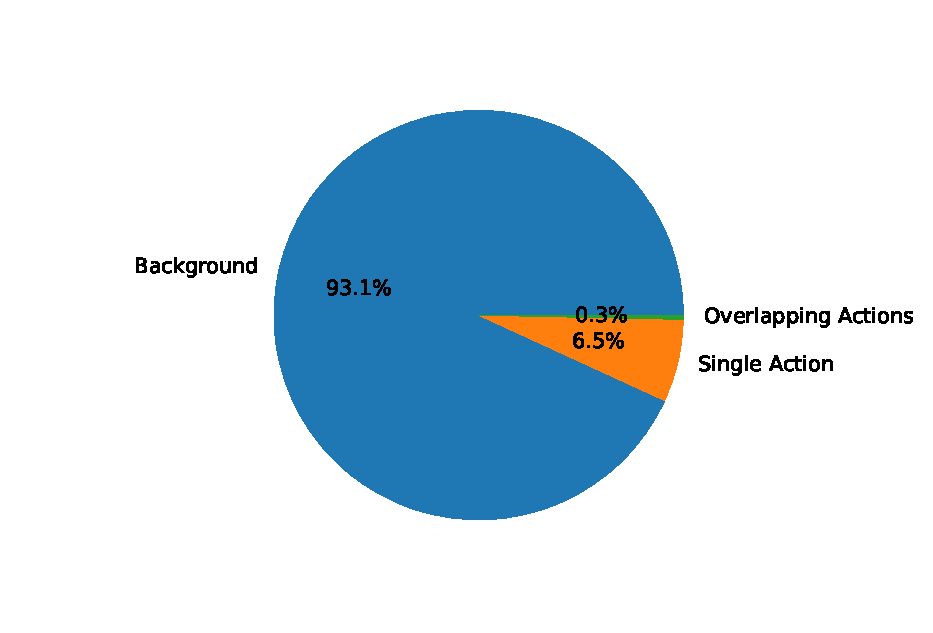
\includegraphics[width=.95\linewidth]{img/data-plots/1sec/background_ratio_all_1sek.eps}
        \caption{$\Delta = 1$}
        %\label{fig:anno_bg_ratio}
    \end{subfigure}%
    \begin{subfigure}{.3\textwidth}
        \centering
        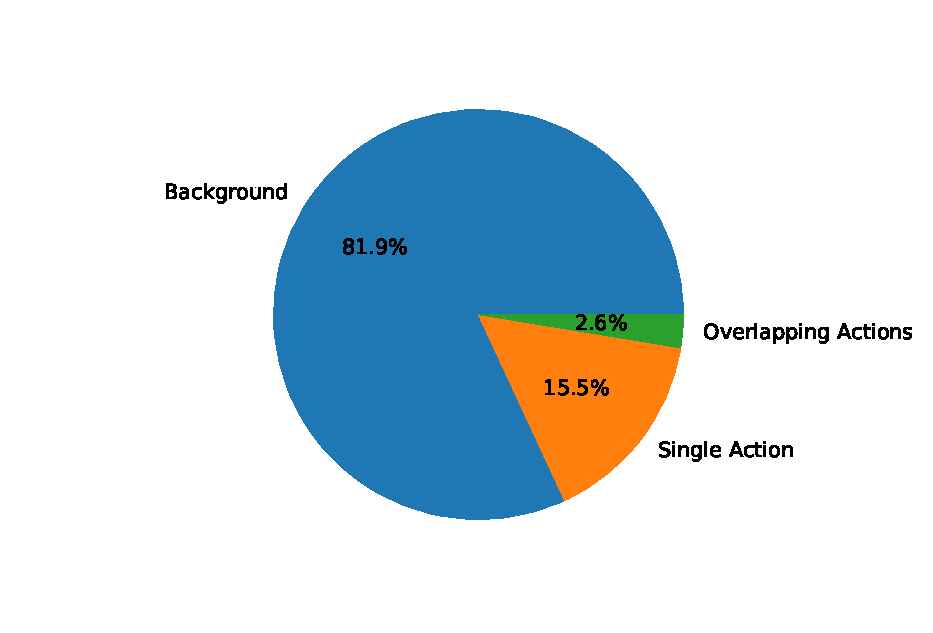
\includegraphics[width=.95\linewidth]{img/data-plots/4sec/background_ratio_all_202010-1419-3706.eps}
        \caption{$\Delta = 4$}
        %\label{fig:anno_classes}
    \end{subfigure}
    \begin{subfigure}{.3\textwidth}
        \centering
        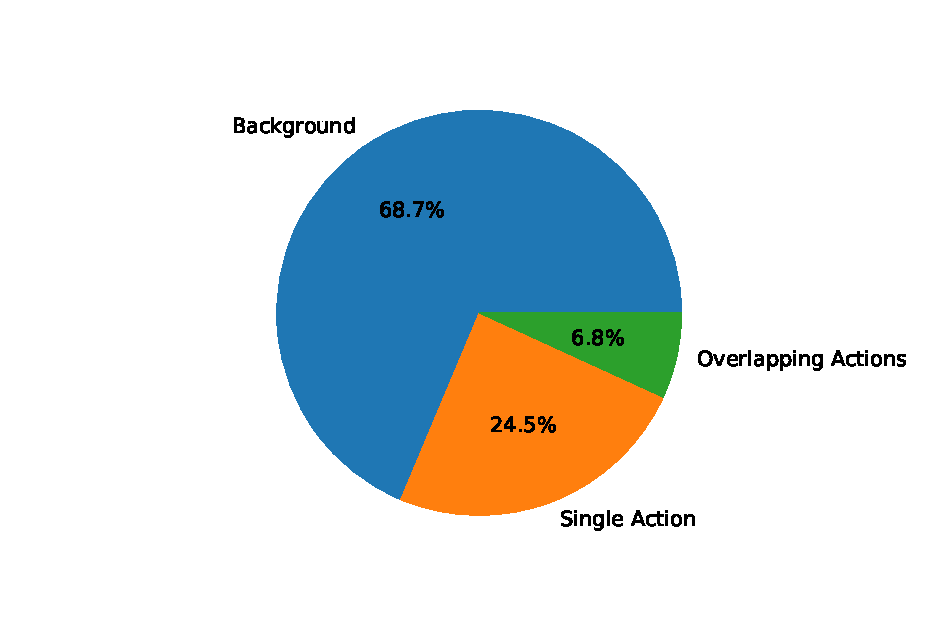
\includegraphics[width=.95\linewidth]{img/data-plots/8sec/background_ratio_all_202010-1419-4303.eps}
        \caption{$\Delta = 8$}
        %\label{fig:anno_classes}
    \end{subfigure}
    \caption{Skalierung des Background- und Überschneidungsverhältnisses zur Wahl von $\Delta$}
    \label{fig:ratios}
\end{figure}

Dass die Zahl der Überschneidungen mit der Wahl von $\Delta$ skaliert, belegt auch der wachsende Anteil von Samples mit mehr als einer Aktion, wie \autoref{fig: ratios} zeigt.
Dabei wird die in \autoref{subsec:segmentierung-und-sampling-strategie} verwendete Sampling-Strategie verwendet.

\begin{figure}
    \centering
    \bigimage{img/data-plots/4sec/pairwise_occurrences_all_202010-1419-3817}{\textwidth}
    \caption{Anteil paarweiser Überschneidungen pro Klasse (hier: $\Delta = 4$)}
    \label{fig:overlaps}
\end{figure}
%% wie wird der einfluss geprüft

Als Folge der oben veranschaulichten Statistiken wird vorab auf ein Multi-Label-Ansatz gesetzt.
Das Verfahren ist damit auch flexibler bei Anpassungen des Aktionskatalogs und kommt ohne ein künstlichen \emph{Background}-Labels aus.
Zudem kann auf ein aufwendiges Verfahren dedizierte, überschneidungsfreie Intervalle für jede Aktion zu finden verzichtet werden.
Stattdessen kann das ungeschnittene Videomaterial gleichmäßig segmentiert werden und jedes Segment erhält Labels für alle darin stattfindenden Aktionen.

\section{Umgang mit Fehlern im Datenset}
\label{sec:umgang-mit-fehlern-in-datenset}

Auch wenn die Annotationen aus \gls{sbod} manuell erfasst und verifiziert wurden, können sie dennoch Fehler enthalten.
Und selbst bei gegebener Fehlerfreiheit, lägen ihnen wahrscheinlich ein anderes als das in dieser Arbeit verwendetes Videomaterial zugrunde.
\gls{sbod} dient zur Auswertung von Spieldaten und ist auf Vollständigkeit aller Aktionen angewiesen.
Der Grundlegende Unterschied zum Datenset dieser Arbeit ist, dass dieses Datenset ausschließlich sichtbare Aktionen umfassen soll.
Als Ground Truth gilt also immer nur das, was in dem jeweiligen Clip wirklich zu sehen ist.
\Dh zum einem dass Aktionen die passiert sind, im Video aber nicht sichtbar sind (\zB weil die Kamera gerade ins Publikum schwänkt), entfernt werden müssen.
Zum anderen bedeutet es, dass Wiederholungen von Aktionen im Video zusätzliche Aktionen darstellen, auch wenn sie sich in der realen Welt zu einem anderen Zeitpunkt ereignet haben.

Damit nicht jeder Datensatz einzeln korrigiert werden muss, wird ein Post-Processing-Schritt in das Trainingssetup aufgenommen.
Während des Trainings werden die Fehler der Loss-Funktion pro Sample protokolliert, sodass im Anschluss nur die Samples mit dem höchsten Fehlerwerten manuell verifiziert und im Fehlerfall korrigiert werden müssen.
Der Ablauf orientiert sich an \cite{Gugger20} und \cite{Cioppa20}, die durch die Ergebnisse der Fehlerfunktion Fehler in den Annotationen von SoccerNet gefunden haben.

\section{Konzeptuelle Umsetzung}
\label{sec:konzeptuelle-umsetzung}

Das \gls{har}-Modell lässt sich in ein modulares Framework integrieren, mit dem ungeschnittene Videos kompletter Halbzeiten verarbeitet werden können.
Das Framework deckt den kompletten Zyklus von der Datenaufbereitung, über das Training bis zur Inbetriebnahme ab.
Das Modell ist dabei gegen eine andere Architektur austauschbar, sofern es eine wohl-definierte Schnittstelle bereitstellt.

Der Endnutzer stellt ein Video in Form einer \gls{url} oder eines Uploads bereit und erhält eine Liste der Spielaktionen.

\begin{figure}[htbp!]
    \centering
    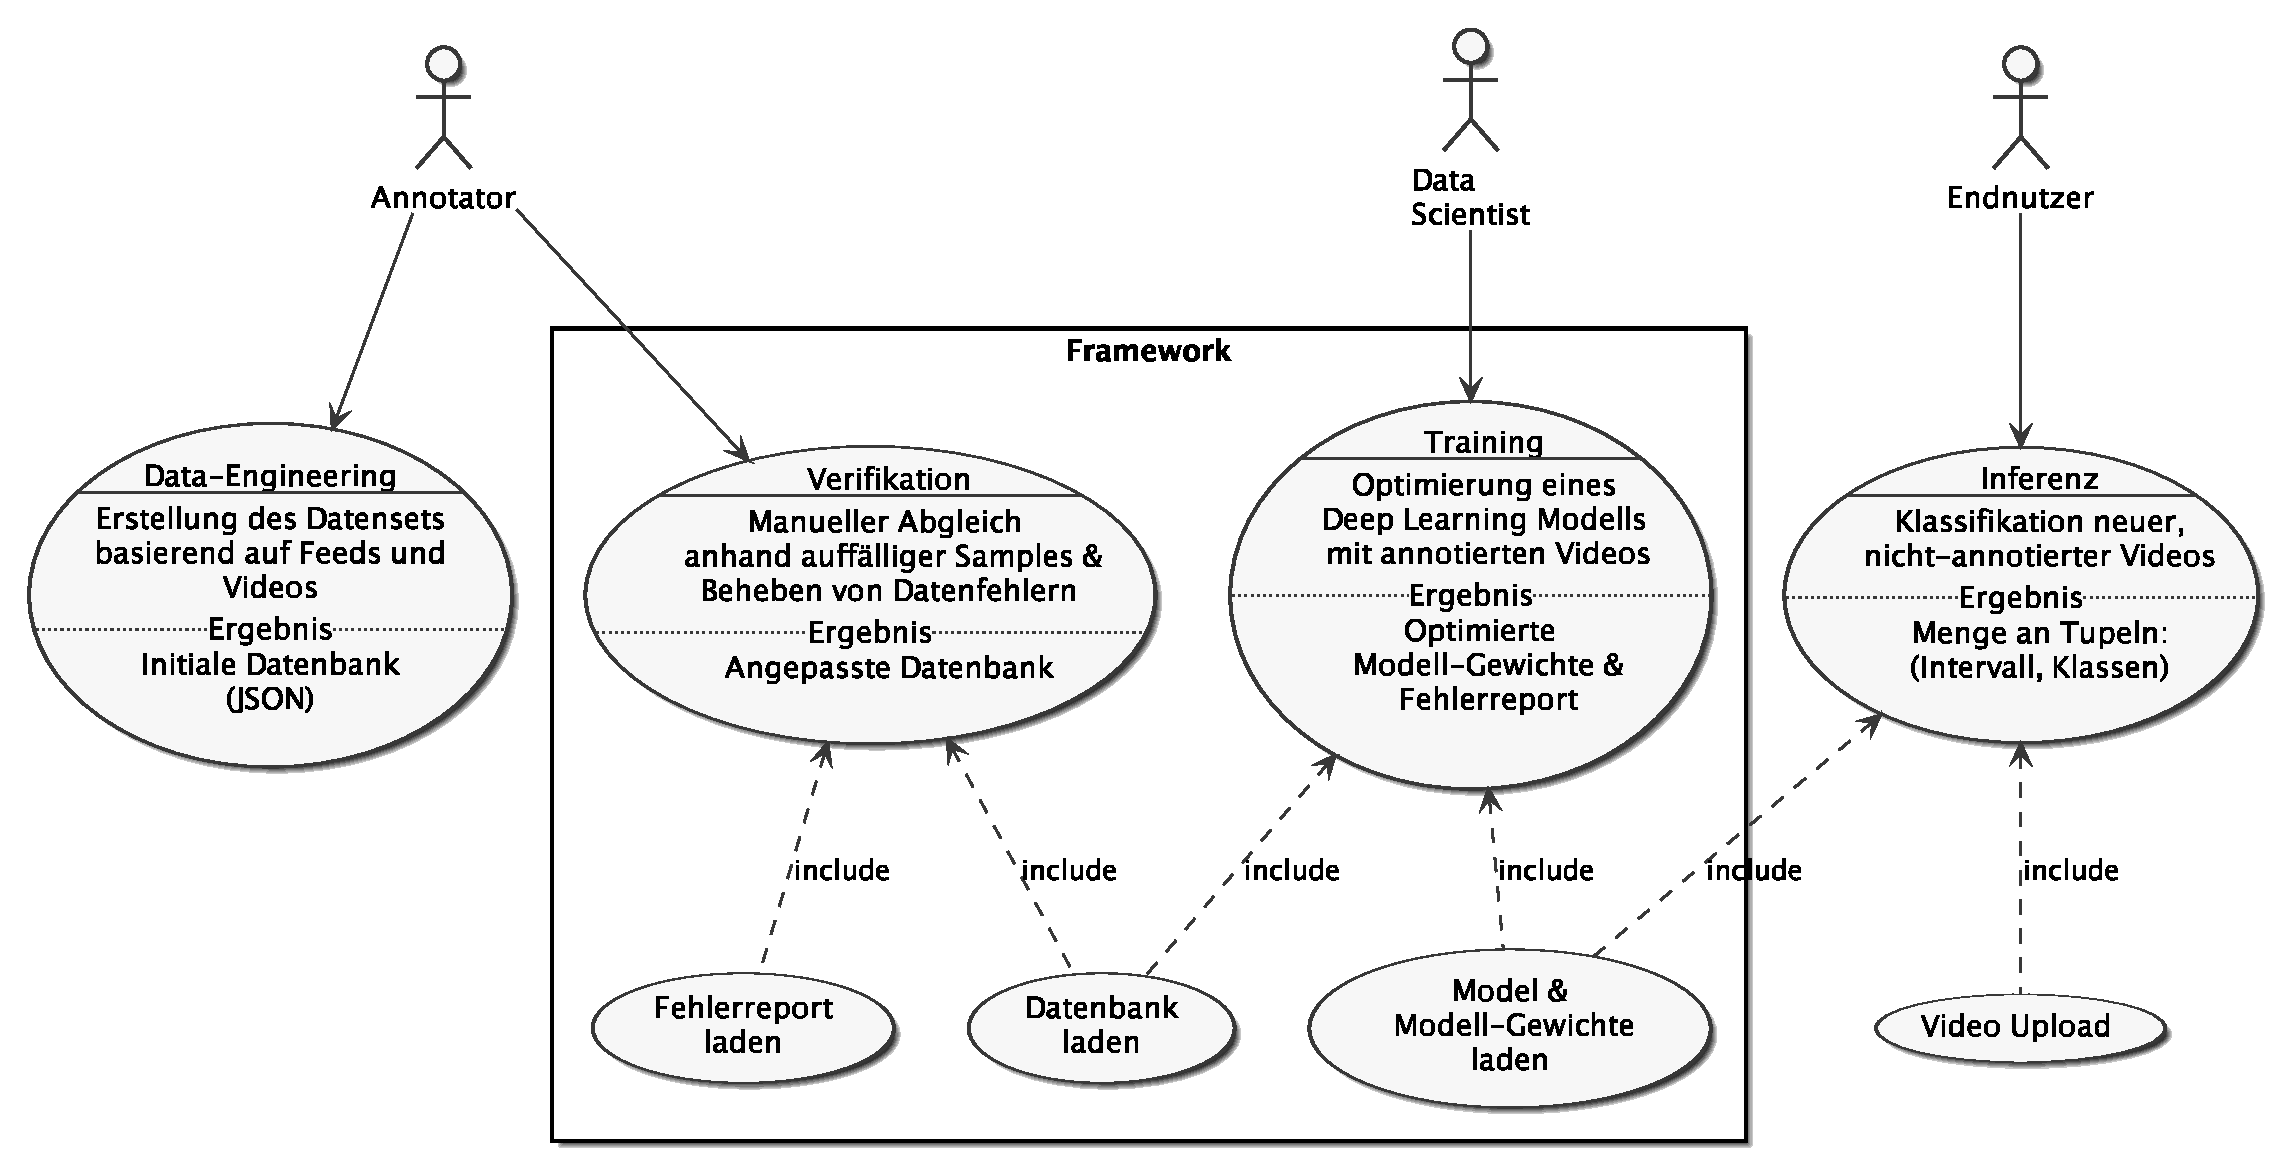
\includegraphics[width=0.9\textwidth, height=0.8\textwidth, keepaspectratio, interpolate]{fig/usecase.eps}
    \caption{Anwendungsfalldiagramm: Framework}
    \label{fig:usecase}
\end{figure}

\autoref{fig:usecase} zeigt die Funktionen aus Anwenderperspektive.

Um alle Experimente in einer generischen Umgebung durchzuführen wurde eine modulare Implementation umgesetzt, die auf dem Konzepten des Frameworks Lightning (\cite{Falcon19}) basiert.
In \autoref{fig:modules} sind die drei Kernmodule zur Datenintegration, dem Training und der Evaluierung, sowie der vorgelagerte Prozess der Datenerfassung schemenhaft veranschaulicht.

\begin{figure}
    \centering
    \bigimage{fig/modules-top}{0.8\textwidth}
    \caption{Module zur konzeptuellen Umsetzung}
    \label{fig:modules}
\end{figure}

Die Hyperparameter aus \autoref{subsec:hyperparameter} sind für das Datenmodul konfigurierbar.
Das Datenmodul beinhaltet Klassen zum Erstellen und Bereitstellen valider Samples, die vom Trainings- und Evaluation-Modul genutzt werden können.

Das Trainingsmodul benutzt die Samples zur Optimierung des \gls{har}-Backbones.
Hervorzuheben ist, dass das \gls{har}-Modell keinerlei Abhängigkeiten zu anderen Komponenten hat und komplett austauschbar ist.

Pro Epoche werden die Scores und Losses aus dem Training an das Evaluationsmodul übergeben.
Das Evaluationsmodul sichert diese Werte zusammen mit den Ground-Truth Labels und weiteren Metadaten in Form eines Reports in einer \gls{csv}-Datei.
Ebenfalls werden Metriken und Statistiken über einen Logging-Mechanismus während des Training an einen Cloud-Speicher\footnote{Ergebnisse unter https://www.comet.ml/narendorf/soccar-32} übermittelt.
Abschließend werden auch Hyperparameter, der Quellcode, die Modellgewichte und der Report in der Cloud gesichert, sodass sich alle Ergebnisse eindeutig reproduzieren lassen.

\chapter{Data-Engineering}
\label{ch:data}

\newcommand{\noaction}{37521\ }
\newcommand{\novideos}{194\ }
\newcommand{\nomatches}{152\ }

In diesem Kapitel werden die Schritte zur Generierung des Datensets SOCC-HAR-32 beschrieben, sowie seine Eigenschaften und weitere Aufbereitungsschritte.
Unter Data Engineering wird das Problem beschrieben, rohe Daten in ein \gls{ml}-Datenset zu transformieren~\cite{Burkov19}.
Dieser Prozess wird im Folgenden in zwei Teilprobleme unterteilt:
\begin{description}
    \item[Datenerhebung] Prozess, indem ein Datenset erstellt wird.
        Dazu werden verschiedene Datenquellen aggregiert und in einer Datenbank einheitlich persistiert.
    \item[Datenaufbereitung] Prozess zur Laufzeit des Trainings.
        Basierend auf dem Datenset, werden die persistierten Daten ausgelesen und dem \gls{har}-Modell in einer effizienten Weise bereitgestellt.
\end{description}

\begin{tcolorbox}[title=WIP]
    \begin{itemize}
        \item Plots (boxplot für Re-sampling, bar-plots drehen, sodass beschriftung leichter lesbar ist)
        \item Aktionskatalog im Anhang
        \item \Dh die Ungleichgewichtungen der realen Welt (insbesondere die Überrepräsentation von Background-Samples) wird auch im Test-Set widergespiegelt.
    \end{itemize}
\end{tcolorbox}


\section{Datenerhebung}
\label{sec:datenerhebung}

Das zu erstellende Datenset basiert auf den drei Datenquellen \gls{sbod}, SoccerNet und YouTube.
\gls{sbod} gibt eine Liste potenzieller Spiele und damit verknüpfter Spielaktionen vor, für welche passendes Videomaterial aus den anderen zwei Quellen gefunden werden muss.

\subsection{Datenschema}
\label{subsec:schema}

\begin{figure}
    \centering
    \bigimage{fig/schema}{0.7\textwidth}
    \caption{Datenbankschema zur Erhebung des Datensets}
    \label{fig:classes}
\end{figure}

Zu diesem Zweck wird zunächst ein einheitliches Datenschema bestend aus Spielen, Videos und Aktionen wie in \autoref{fig:classes} definiert.
Das Format bezieht sich auf die Speicherung aller Datenquellen in einer dokumentenbasierten NoSQL-Datenbank.

In SoccerNet werden stets zwei Videos pro Spiel bereitgestellt, wobei ein Video jeweils eine der zwei Halbzeiten zeigt.
Da diese Aufteilung nicht immer durch YouTube gegeben ist, werden im Falle eines kompletten Videos über beide Halbzeiten dennoch zwei Datensätze erstellt.
Beide Datensätze weisen dann die gleiche \code{externalId} (die sich aus der Video-\gls{url} ergibt) auf, markieren mit unterschiedlicher \code{startTime} und \code{endTime} jedoch disjunkte Intervalle innerhalb des Videos.

Die gesuchten Aktionsintervalle ergeben sich aus den Feldern \code{second} und \code{duration} und beziehen sich auf die jeweilige Spielzeit, beginnend mit dem Anpfiff der jeweiligen Halbzeit.
Die Zuordnung von Aktionen zu einem Teil-Datenset (\code{split}, hier: Trainings-, Validierungs-, Testset) geschieht Spiel-übergreifend.
\Dh alle Aktionen innerhalb eines Spiels werden stets dem gleichen Datenset zugeordnet.
Diese gängige Praxis wurde übernommen aus~\cite{Giancola18} und~\cite{Jiang19}.

\subsection{Verarbeitungs-Pipeline}
\label{subsec:pipeline}

Um die verschiedenen Datenquellen in das beschriebene Format zu überführen, wird ein semi-automatisierter Datenimport ausgeführt, deren Schritte in \autoref{fig:collection-pipeline_a} dargestellt sind.
Dieser überführt zunächst alle Spiele aus \gls{sbod} in das obige Datenschema.
Anschließend werden zwei Provider-Klassen (für SoccerNet und YouTube) implementiert, pro Spiel mehrere Stufen einer Import-Pipeline durchlaufen (\autoref{fig:collection-pipeline_b}), in denen weitere Datensätze angelegt werden.
Zuletzt werden die relationalen Daten aus der Datenbank in eine JSON-Datei exportiert.

\begin{figure}
    \centering
    \begin{subfigure}[b]{.5\textwidth}
        \centering
        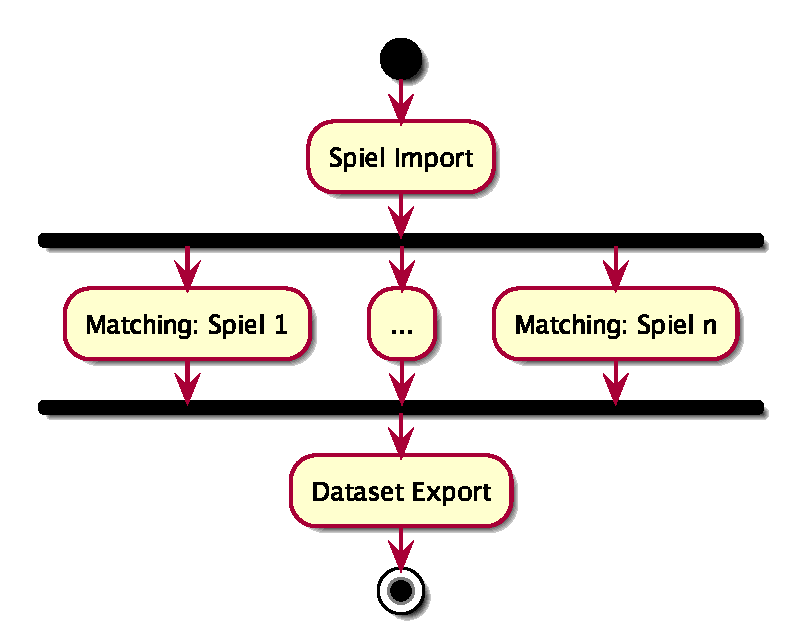
\includegraphics[width=.8\linewidth]{fig/collection.eps}
        \caption{Gesamter Prozess}
        \label{fig:collection-pipeline_a}
    \end{subfigure}%
    \begin{subfigure}[b]{.5\textwidth}
        \centering
        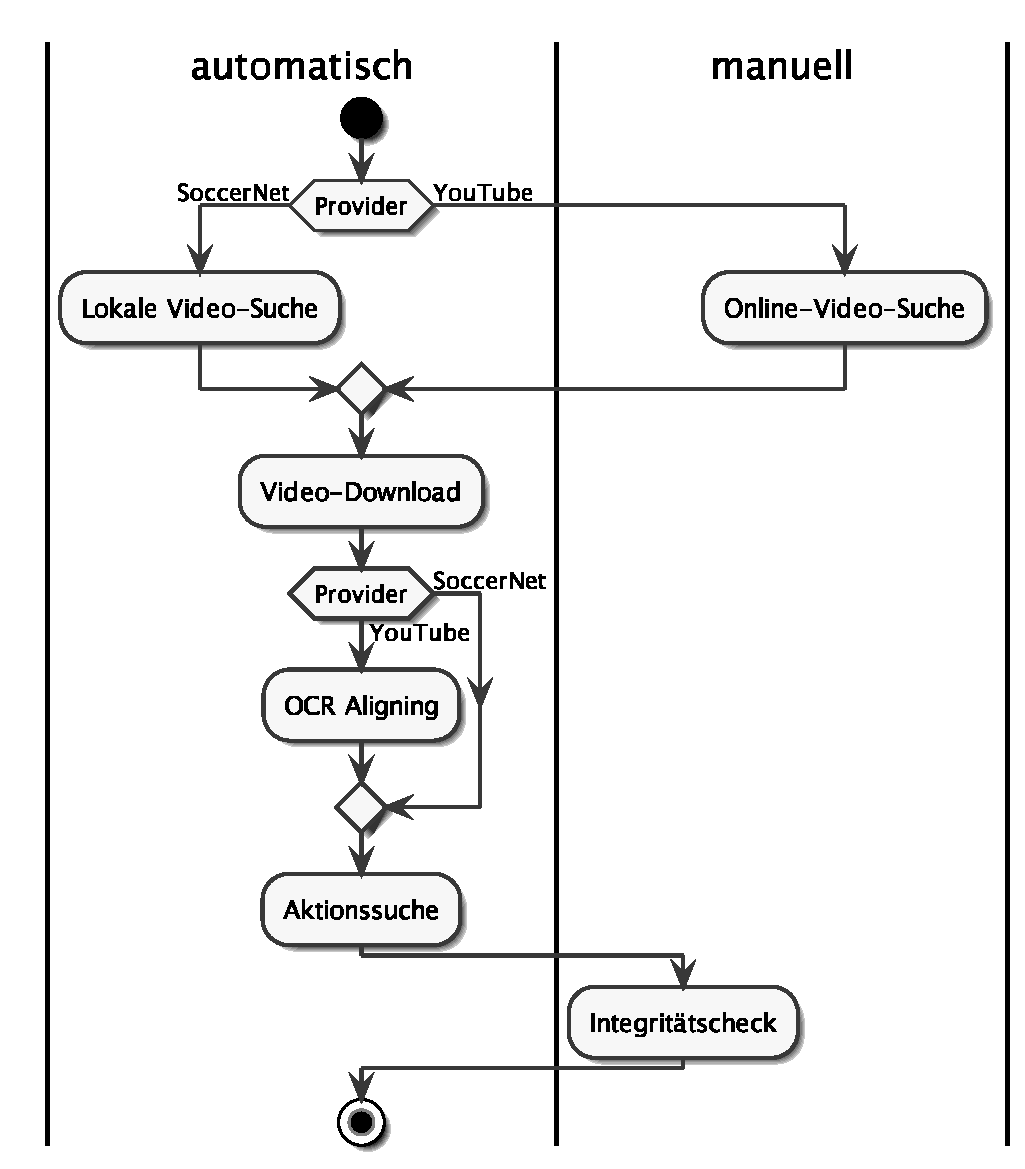
\includegraphics[width=.95\linewidth]{fig/collection-pipeline.eps}
        \caption{Matching pro Spiel}
        \label{fig:collection-pipeline_b}
    \end{subfigure}
    \caption{Pipeline zur Datenerhebung}
    \label{fig:collection-pipeline}
\end{figure}

Im ersten Schritt der Import-Pipeline wird ein Matching durchgeführt, welches prüft, ob es eine Überschneidung der Daten gibt.
Für den SoccerNet-Provider reicht ein lokaler Abgleich zwischen den online\footnote{https://github.com/SilvioGiancola/SoccerNet-code (Stand: 08.10.2020)} verfügbaren Dateilisten mit einem Suchbegriff -- bestehend aus Wettbewerb, Saison, Mannschaften, Spieldatum und Ergebnis.
Gibt es eine Übereinstimmung werden die Attribute \code{provider} und \code{externalId} des Matches gespeichert und jeweils zwei neue Video-Datensätze generiert.
Alle dieser Videos sind in je einer niedrigen (224p) und in einer hohen Qualität (720p oder 1080p) online verfügbar.
Zusätzlich wird pro Halbzeit eine Textdatei bereitgestellt, die den Zeitpunkt des An- und Abpfiffs innerhalb des Videos angibt.
Diese Informationen werden im jeweiligen Video-Datensatz als \code{startTime} bzw. \code{endTime} gespeichert.

Gibt es keine Übereinstimmung, wird auf den YouTube-Provider zurückgegriffen, der eine Online-Video-Suche anstößt.
Da Videos auf YouTube nicht für diese Aufgabe verifiziert sind, kann dieser Schritt nicht vollautomatisiert, sondern nur semi-automatisiert geschehen.
In einer \gls{gui} werden dem Nutzer mehrere Videos als Suchtreffer der YouTube-\gls{api} vorgeschlagenen.
Diese Videos kann der Nutzer mit den Eigenschaften des Match-Datensatzes (Datum, Ergebnis, Saison, etc.) manuell abgleichen und im Falle eines Matchings einer der Halbzeiten oder (falls das komplette Spiel gezeigt wird) beiden Halbzeiten zuordnen.
Wird bei keinem der Provider ein Treffer gefunden, wird das Spiel wieder aus der Datenbank gelöscht.

Im nächsten Schritt werden die Video-Dateien beider Halbzeiten in der höchstmöglichen Auflösung von der jeweiligen Plattform heruntergeladen und lokal zwischengespeichert.
Für alle Videos, die nicht vom SoccerNet-Provider kommen und somit noch keine \code{startTime} und \code{endTime} haben, wird die Startzeit der Halbzeit automatisiert mittels \gls{ocr} wie folgt bestimmt:

\subsubsection{Aligning mit OCR}

Damit die verfügbaren \gls{annotationen} mit den Video-Daten in Beziehung gesetzt werden können, müssen beide Datenquellen den gleichen zeitlichen Nullpunkt aufweisen.
Dieses Problem wird als Aligning bezeichnet~\cite{Purushwalkam20}.
Die \gls{sbod}-\gls{annotationen} bestimmen für jede Aktion einem Zeitpunkt gemessen an der Spieluhr (Spielzeit).
Die Videos selbst starten allerdings in der Regel schon wenige Minuten vor dem Anpfiff (Videozeit).
Als gemeinsame Nullpunkt wird deshalb der Anpfiff der jeweiligen Halbzeit festgesetzt.

In jedem Video befindet sich oben rechts oder oben links eine Spielzeitanzeige.
Der Nullpunkt im Video ist genau eine Sekunde bevor die Anzeige von \emph{00:00} aus \emph{00:01} umschlägt.

Um diesen Zeitpunkt schnell und genau zu finden, werden Screenshots verschiedener Frames erstellt, aus welchen mittels \gls{ocr} der Text des Bildbereichs extrahiert, indem typischerweise die Spieluhr zu finden ist.
Dieser Text, der immer dem Schema einer Uhrzeit entspricht, wird mit einem Regulären Ausdruck in Sekunden-Einheiten konvertiert, aus denen sich wiederum die Differenz von Videozeit zur Spielzeit ergibt.
Wiederholt man diesen Prozess oft genug, nähert sich der Median dieser Differenzen dem gesuchten Nullpunkt für den Anpfiff der ersten \bzw zweiten Halbzeit an.
Der Nullpunkt wird als \code{startTime} gespeichert, während sich die \code{endTime} aus Startzeit und Dauer der Halbzeit ergibt, wobei die Halbzeitdauer wiederum in den \gls{sbod}-\gls{annotationen} enthalten ist.
Der Einsatz einer \gls{ocr} wurde in ähnlicher Form auch in~\cite{Giancola18} für den gleichen Zweck genutzt.
Für die Umsetzung bedient sich diese Arbeit an der Open-Source-Bibliothek Tesseract~\cite{Smith07}.

\subsubsection{Aktionssuche}

An dieser Stelle der Pipeline können \gls{annotationen} und Videos miteinander kombiniert werden.
Daher werden im nächsten Schritt alle Aktionen eines Spiels vom Datenprovider \gls{sbod} geladen.
Diese externen, aus den 33 Oberkategorien bestehenden Klassendefinitionen \cite{StatsbombDocs16} werden in neu abgeleitete Aktionsklassen transformiert.

In \autoref{lst:sbod} ist ein exemplarischer Auszug, der eine Annotation aus \gls{sbod} zeigt.
Die Aktionsdatensätze der Datenbank beinhalten neben der \code{externalClass} (hier: übernommen aus Zeile 10), auch die weiteren Aktionsdetails (hier: ab Zeile 26) als \code{details}, aus denen neue, eigene Aktionsklassen abgeleitet werden.
Die neuen Aktionen werden durch einen Query-Selektor im MongoDB-Format\cite{Bradshaw16} definiert.
Mit dem Selektor können alle \gls{annotationen} dieser Klasse in einem Zug aus den \gls{sbod}-\gls{annotationen} eines Spiels, die in separaten Dateien vorliegen, gefiltert werden.
Die Repräsentation als Selektor ist unabhängig vom hier benutzten Datenschema und der Programmiersprache und lässt sich auch direkt auf die \gls{json}-\gls{annotationen} in \gls{sbod} anwenden.

%\lstinputlisting[language=json, caption=Datenformat in SoccerNet]{code/soccernet.json}
%\label{src:soccernet}

\lstinputlisting[language=json, label=lst:sbod, caption=Datenformat in Statsbomb Open Data]{code/sod.json}

\subsubsection{Integritätscheck}

Abschließend wird manuell noch die Überlagerung von Aktionen und Videos manuell kontrolliert.
Dabei wird geprüft, ob das Aligning korrekt ist, indem der Nutzer pro Halbzeit die Videozeit der ersten und letzten Spielminute in einer \gls{gui} verifiziert.
Dazu wird das Video in die \gls{gui} geladen und es wird zu der jeweiligen Stelle im Video gesprungen, in der das Aligning die zweite \bzw letzte Spielminute vermutet.
Sieht der Nutzer nun \zB die Spieluhr mit der Anzeige \emph{01:00} bzw. \emph{44:00} (bei punktgenauem Abpfiff) kann er das Alignment verifizieren.
Dadurch wird sichergestellt, dass keine Spielminuten aus dem Video herausgeschnitten wurden und dass die Abspielgeschwindigkeit der Originalgeschwindigkeit entspricht.

Als zweiter Integritätscheck wird geprüft, ob der zeitliche Nullpunkt dem tatsächlichen Anstoß entspricht.
Während der Entwicklungsphase hat sich herausgestellt, dass die eingeblendete Spieluhr nur in 7 \% der Fälle mit dem Anstoß beginnt zu zählen.
In 2,3 \% der Fälle startet sie bereits früher und in 90,8 \% erst später.
Die \gls{annotationen} in \gls{sbod} beziehen sich auf den \emph{echten} Nullpunkt, welcher sich durch den Anstoß definiert, was die Ergebnisse des vorherigen Alignings diskreditiert.
Denn ein fehlerhaftes Alignment führt zu einer systematischen Verschiebung aller Aktionsintervalle entlang der Zeitachse.

Um den potenziell falsch ermittelten Nullpunkt des Alignings zu korrigieren, kann der Nutzer den Nullpunkt in der \gls{gui} um wenige Sekunden nach vorne oder nach hinter justieren.
Zur Orientierung werden die Aktionen dabei unter dem Video in einer Zeitleiste eingeblendet.

Ist der Integritätscheck durch den Nutzer abgeschlossen, wird das Spiel einem der drei Datensubsets (Trainings-, Validierungs- und Testset) zugewiesen.
Bei Überschneidungen mit SoccerNet wird die Original-Zuteilung übernommen.
In allen anderen Fällen geschieht die Zuweisung zufällig unter der Gewichtung $3:1:1$ -- wie in~\cite{Giancola18}.

\subsubsection{Export}

Der letzte Schritt der Datenerhebung ist der Export in ein kompaktes Dateiformat, welches die Schnittstelle für weitere Anwendungen darstellt.
Das Zielformat ist eine Art Erweiterung des Speicherformats in~\cite{Caba15} (basierend auf JSON).
\autoref{fig:storage-format} zeigt das Format und hebt die Änderungen in Vergleich zum Basisformat hervor.

\begin{figure}
    \centering
    \bigimage{fig/storage}{0.7\textwidth}
    \caption{Dateiformat zur Speicherung des Datensets}
    \label{fig:storage-format}
\end{figure}

Die Liste der Klassen wird durch die in \autoref{subsec:pipeline} genannten Selektoren erweitert.
Die eigentliche Datenbank speichert Einträge pro Halbzeit in einer Map, wobei sich der Schlüssel der externen Spiel-ID aus \gls{sbod} und der Nummer der Halbzeit zusammensetzt.
Pro Halbzeit kann über die \gls{url} auf das Video geschlossen werden.
Da sich das Video potenziell mit der anderen Halbzeit desselben Spiels überschneidet, wurden zusätzlich die Start- und Endzeit der Halbzeit unter \code{segment} gespeichert.
Jede Videohälfte referenziert nun eine Liste der darin enthaltenen Aktionen mit jeweils dem \code{label} und einem \code{segment} bestehend aus Start- und Endmarkierung.
Zusätzlich wird auch hier ein eindeutiger Identifier in Form einer \gls{url} definiert, um das Debugging zu erleichtern.

\section{Eigenschaften des Datensets}
\label{sec:eigenschaften-des-datensets}

Das Resultat der Datenerhebung ist ein Datenset, welches \noaction Aktionen und \novideos Videos aus insgesamt \nomatches Spielen umfasst.
In \autoref{tab:action} werden alle 32 Klassen des Datensets aufgelistet.
Neben der Anzahl ist die durchschnittliche und maximaler Dauer pro Aktion vermerkt, die sich aus den \gls{annotationen} in~\cite{Statsbomb20} ergeben.
Aktionen, die hier keinen Wert vorweisen werden lediglich als Zeitpunkt in \gls{sbod} repräsentiert.

\begin{figure}
    \centering
    \small
    \begin{subfigure}{0.45\textwidth}
        \centering
        \csvautotabular{tbl/actions_a.csv}
    \end{subfigure}
    \begin{subfigure}{0.45\textwidth}
        \centering
        \csvautotabular{tbl/actions_b.csv}
    \end{subfigure}
    \caption{Aktionskatalog in SOCC-HAR-32}
    \label{tab:action}
\end{figure}

\subsection{Ungleichverteilung von Aktionen}
\label{subsec:ungleichverteilung-von-aktionen}

Trotz der hohen Zahl an Aktionsklassen, besteht der Hauptteil des Videomaterials aus aktionsfreien Teilen (Background).
\autoref{fig:anno_bg_ratio} zeigt das Verhältnis von durch Aktionen geprägter Videozeit bei einsekündiger Segmentierung aller Halbzeitvideos.
Die Zeit vor und nach den Halbzeiten wird nicht mitgezählt.
Hinzu kommt, dass die Klassen untereinander sehr ungleich verteilt sind, wie \autoref{fig:anno_classes} zeigt.
Die genauen Zahlen sind ebenso der Tabelle in \autoref{tab:action} zu entnehmen.

\begin{figure}
    \centering
    \begin{subfigure}{.5\textwidth}
        \centering
        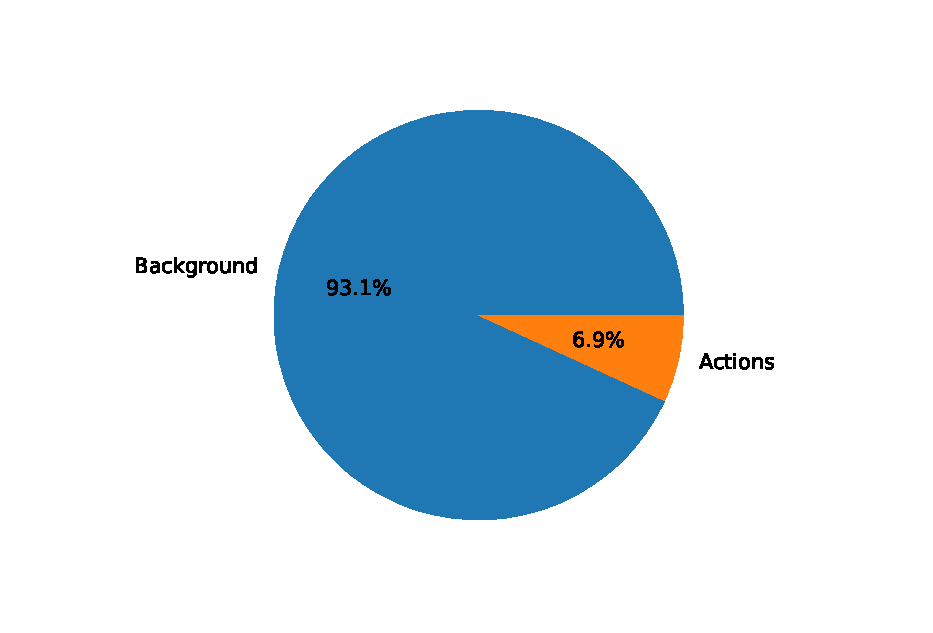
\includegraphics[width=.9\linewidth]{img/data-plots/background_ratio_all_annos.eps}
        \caption{Anteil der Aktionen im Videomaterial}
        \label{fig:anno_bg_ratio}
    \end{subfigure}%
    \begin{subfigure}{.5\textwidth}
        \centering
        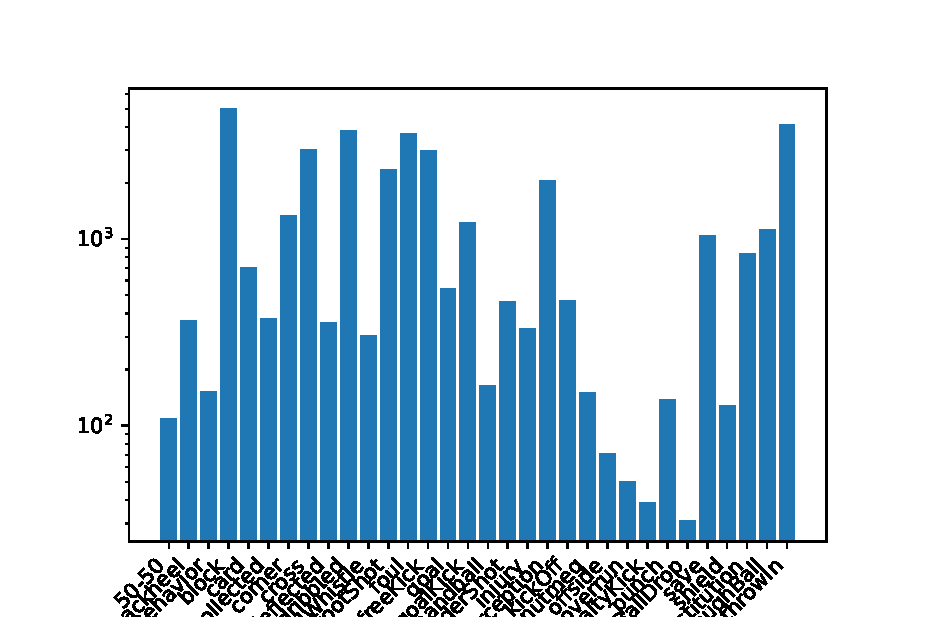
\includegraphics[width=.95\linewidth]{img/data-plots/class_distribution_annotations_all.eps}
        \caption{Verteilung der Klassen}
        \label{fig:anno_classes}
    \end{subfigure}
    \caption{Eigenschaften zum Datenset}
    \label{fig:annotations}
\end{figure}


\subsection{Überschneidungen von Aktionen}
\label{sec:multi-label}

Der oben genannte Aktionskatalog hat mit insgesamt 32 Aktionsklassen das Potenzial einige Aktionen zu beinhalten, die sich mit anderen zeitlich überschneiden.
Dazu zählt einerseits der Fall, dass zwei Aktionen von zwei verschiedenen Spielern tatsächlich zeitgleich ausgeführt werden.
Andererseits können abhängig von der Problembeschreibung \zB hierarchische Klassen definiert werden, sodass sich eine Klasse \code{penaltyKick} immer mit der Klasse \emph{footShot} überlagert.

Um die Signifikanz dieses Problems zu verdeutlichen wurden untersucht, wie sich die Wahl von $\Delta$ auf die Anzahl von Überschneidungen auswirkt.
\autoref{fig:ratios} zeigt, dass bei einem höheren Zeitkontext $\Delta$ die Zahl von Hintergrund-Samples zwar sinkt, die Zahl der Überschneidungen jedoch steigt.

Als Folge der oben veranschaulichten Statistiken wird vorab auf ein Multi-Label-Ansatz gesetzt.
Das Verfahren ist damit auch flexibler bei Anpassungen des Aktionskatalogs und kommt ohne ein künstlichen \emph{Background}-Labels aus.
Zudem kann auf ein aufwendiges Verfahren dedizierte, überschneidungsfreie Intervalle für jede Aktion zu finden, verzichtet werden.
Stattdessen kann das ungeschnittene Videomaterial gleichmäßig in Clips segmentiert werden und jeder Clip erhält ein Label pro darin stattfindender Aktion.

Zudem wurde untersucht, wie oft sich eine Klasse mit einer anderen überschneidet.
Eine dedizierte Grafik ist in \autoref{ch:overlaps} zu finden.
Die häufigsten Kombinationen sind (bei $\Delta=4$) folgende:

\begin{enumerate}
    \item \code{saved} mit \code{footShot}: 74 \%
    \item \code{penaltyKick} mit \code{goal}: 57 \%
    \item \code{badBehavior} mit \code{card}: 51 \%
    \item \code{goal} mit \code{footShot}: 50 \%
    \item \code{collected} mit \code{cross}: 40 \%
\end{enumerate}

\begin{figure}
    \centering
    \begin{subfigure}{.3\textwidth}
        \centering
        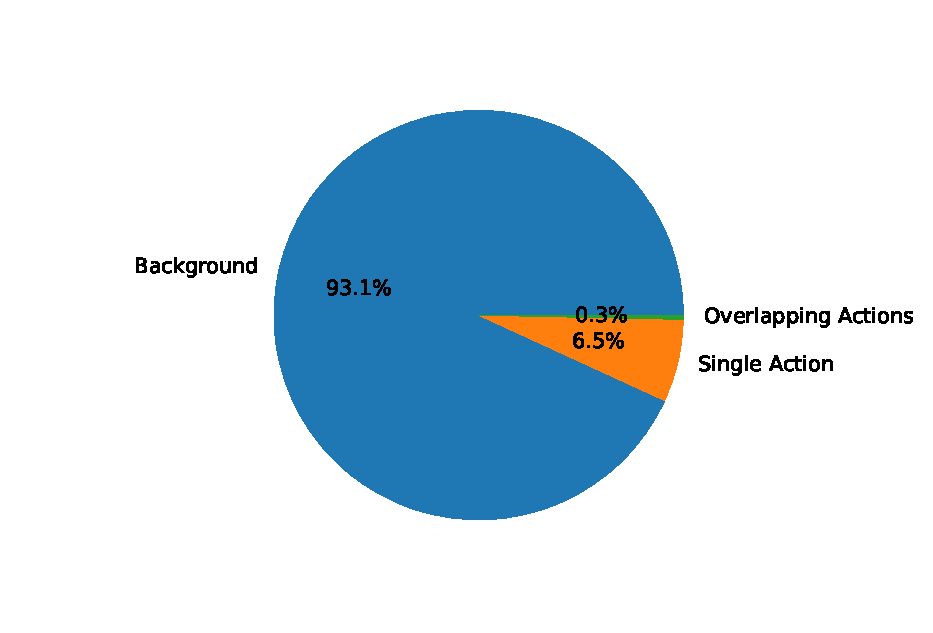
\includegraphics[width=.95\linewidth]{img/data-plots/1sec/background_ratio_all_1sek.eps}
        \caption{$\Delta = 1$}
        %\label{fig:anno_bg_ratio}
    \end{subfigure}%
    \begin{subfigure}{.3\textwidth}
        \centering
        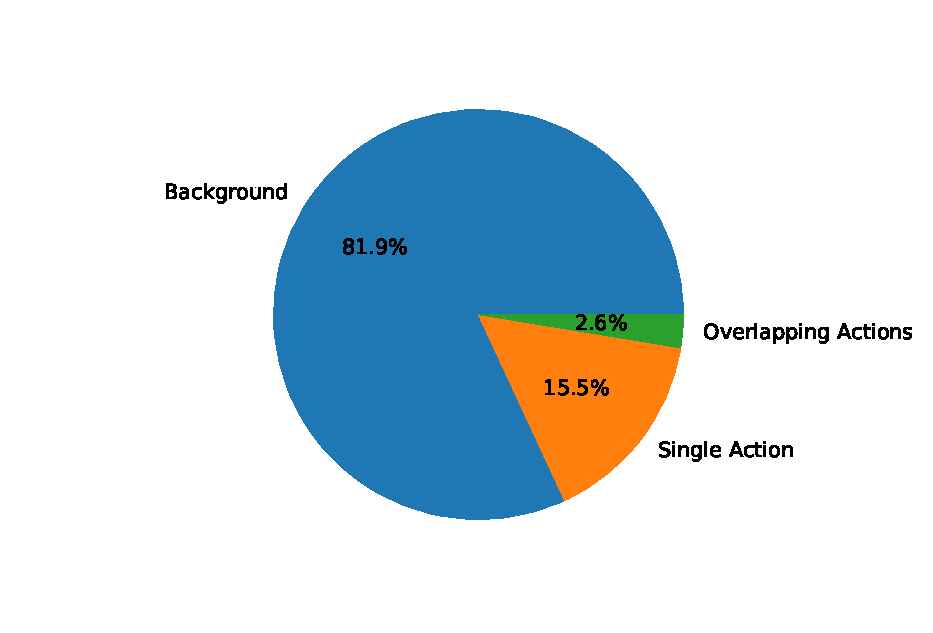
\includegraphics[width=.95\linewidth]{img/data-plots/4sec/background_ratio_all_202010-1419-3706.eps}
        \caption{$\Delta = 4$}
        %\label{fig:anno_classes}
    \end{subfigure}
    \begin{subfigure}{.3\textwidth}
        \centering
        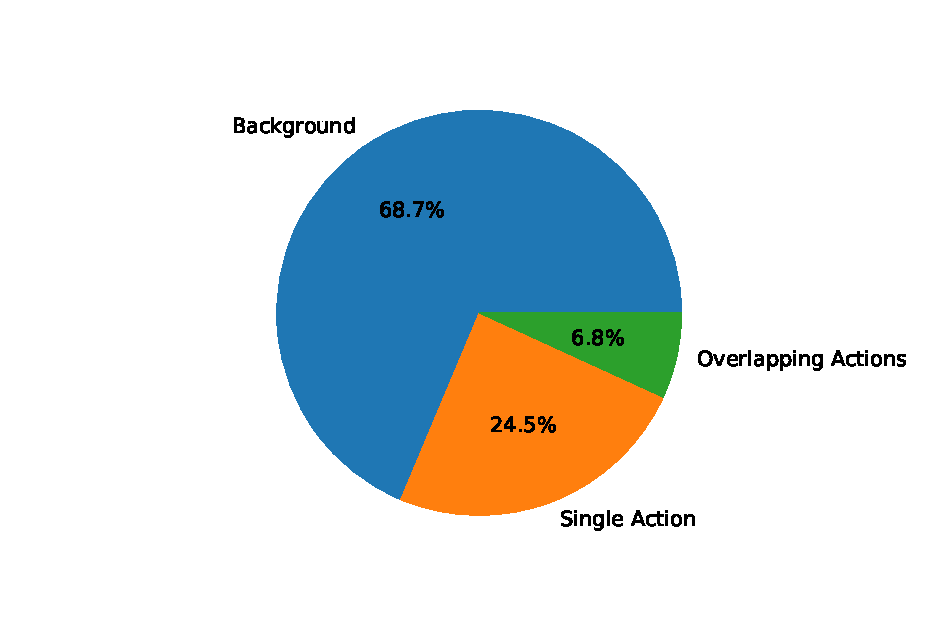
\includegraphics[width=.95\linewidth]{img/data-plots/8sec/background_ratio_all_202010-1419-4303.eps}
        \caption{$\Delta = 8$}
        %\label{fig:anno_classes}
    \end{subfigure}
    \caption{Skalierung des Background- und Überschneidungsverhältnisses zur Wahl von $\Delta$}
    \label{fig:ratios}
\end{figure}

\section{Datenaufbereitung}
\label{sec:pre-processing}

Die Datenaufbereitung basiert auf dem exportierten Datenset des vorherigen Kapitels.
Es umschließt einmalige Prozesse, sowie Prozesse, die pro Training oder pro Sample während des Trainings durchgeführt werden.
\autoref{fig:data-pipeline} zeigt die Prozesse jeder dieser Kategorien.

\begin{figure}
    \centering
    \bigimage{fig/data-pipeline}{0.7\textwidth}
    \caption{Pipeline zum Pre-Processing basierend auf Annotationen}
    \label{fig:data-pipeline}
\end{figure}

\subsection{Effizientes Laden und Speichern}
\label{subsec:effiziente-speicherung}

Um Samples $(x_i, y_i)$ aus den Videos des Datensets zu generieren, müssen einzelne Frames aus den Videos extrahiert und in den Arbeitsspeicher geladen werden.
Dieser Prozess wiederholt sich für jedes Sample pro Epoche, die trainiert wird und stellt ohne weitere Optimierungen einen enormen IO-Overhead dar, der die Geschwindigkeit des eigentlichen Trainings ausbremsen kann~\cite{Wu20}.
Der IO-Zugriff kann \zB reduziert werden, indem die relevanten Frames vorab extrahiert und als Bilder gespeichert werden.
Dieses Vorgehen skaliert jedoch nur mäßig mit der Größe des Datensets, da die Bilder schon bei kleinen Datensets oft zu viel Speicherplatz einnehmen.
Alternativ kann der Zugriff durch Multiprocessing optimiert werden und indem die Videos vorher analysiert werden.
Sind Framerate und \gls{pts} eines Videos bekannt, kann mithilfe des \gls{pes} die entsprechende Stelle innerhalb des Videos direkt und vergleichsweise schnell gefunden werden~\cite{Fischer10}.
Diese Methode ist in den einschlägigen \gls{har}-Bibliotheken (darunter auch die Implementationen von~\cite{Feichtenhofer18} und~\cite{Wang19}) gängige Praxis und wird in diesem Setup übernommen.

Da die Videos nun on-demand dekodiert werden müssen, werden die Videos schon im Vorhinein in einer geringen Auflösung heruntergeladen werden.
Als Zielauflösung wird 360p festgelegt, da es immer noch ein Cropping des höchstauflösenden Modells (mit $S=312$) zulässt und gleichzeitig eine gängige Auflösung des Providers YouTube ist.

Die Videos des Providers YouTube können direkt in der Zielauflösung heruntergeladen werden.
Die Videos des Providers SoccerNet müssen hingegen erst in High Definition heruntergeladen werden und anschließend in die Zielauflösung konvertiert werden.
Alle Videos haben eine einheitliche Framerate von 25 \gls{fps}.
Sobald ein Video in der Zielauflösung verfügbar ist, kann es analysiert werden.
Dazu werden die \gls{pts} und weitere Metadaten erhoben und in einer Pickle-Datei \cite{Lubanovic19} persistiert.

\subsection{Segmentierung und Sampling-Strategie}
\label{subsec:segmentierung-und-sampling-strategie}

Sind Videos und Metadaten lokal verfügbar, können die ungeschnittenen Videos zu \glspl{clip} segmentiert und gelabelt werden.
Die \glspl{clip} werden in einer konfigurierbaren Länge $T$ und Framerate gesamplet.
Um mehrere Samples aus den zugrundeliegenden \gls{annotationen} zu generieren, werden die \glspl{clip} mit einer Verschiebung von einer Sekunde gesamplet.
Das hat zur Folge, dass sich die \glspl{clip} (bei $T > \text{Framerate}$) überschneiden (Temporale Augmentation, siehe~\cite{Giancola18}) und so zusätzliche Samples aus der begrenzten Zahl an Annotationen entstehen.
\autoref{fig:samples} vergleicht pro Klasse die Anzahl möglicher Samples zur Anzahl bestehender \gls{annotationen} bei einer Dauer von $\Delta=4$ Sekunden.

\begin{figure}
    \centering
    \begin{subfigure}{.5\textwidth}
        \centering
        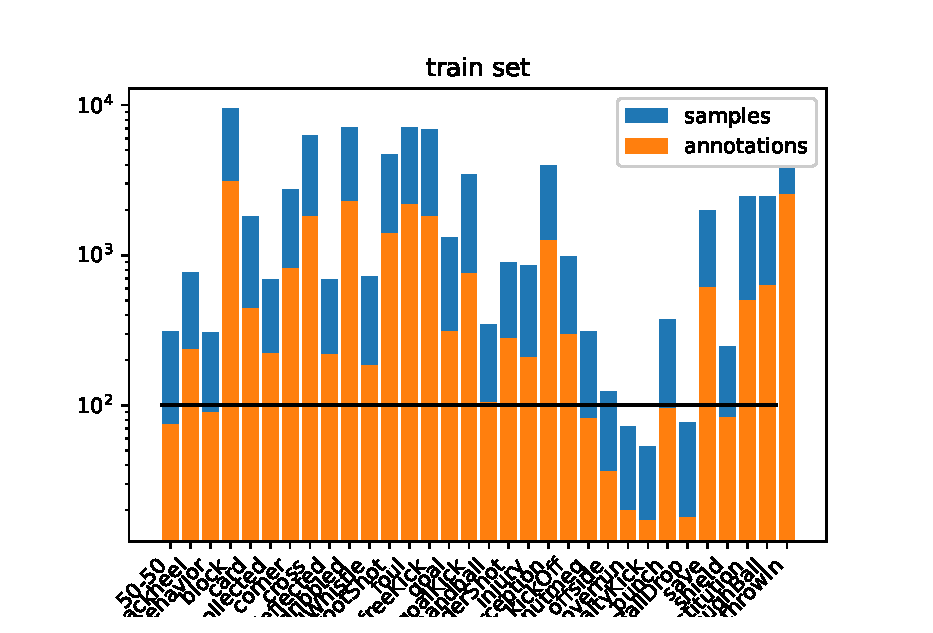
\includegraphics[width=.95\linewidth]{img/data-plots/4sec/class_distribution_annotations_train_202010-1419-3737.eps}
        \caption{Trainingsdaten}
        %\label{fig:anno_bg_ratio}
    \end{subfigure}%
    \begin{subfigure}{.5\textwidth}
        \centering
        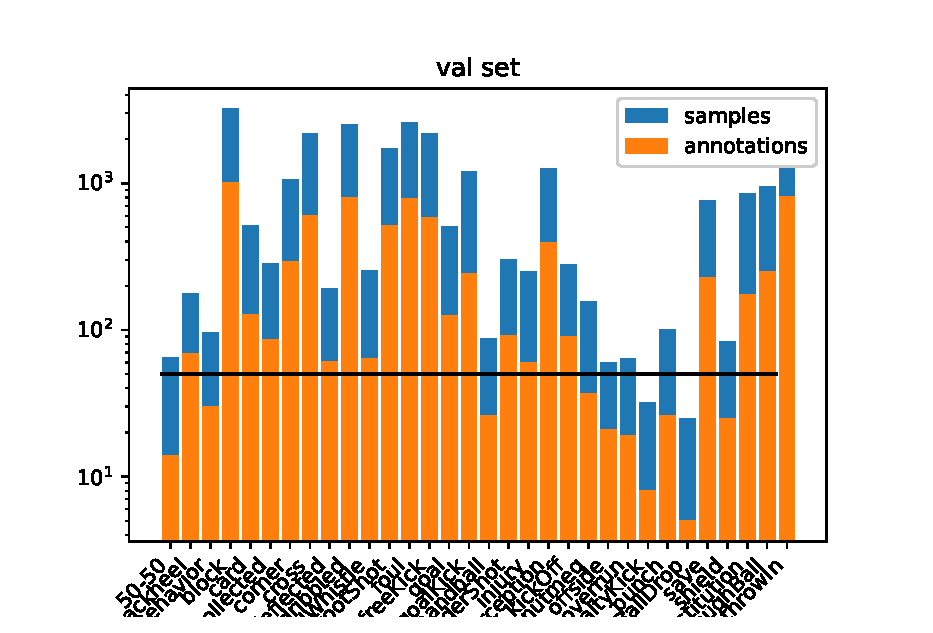
\includegraphics[width=.95\linewidth]{img/data-plots/4sec/class_distribution_annotations_val_202010-1419-3747.eps}
        \caption{Validierungsdaten}
        %\label{fig:anno_classes}
    \end{subfigure}
    \caption{Generierung zusätzlicher Samples aus den Annotationen (bei $\gls{tld:Delta} = 4.0$)}
    \label{fig:samples}
\end{figure}

Diese potenziellen Samples werden intern als Tripel aus Videopfad, Framerate und \gls{pts} gespeichert.
Da die Trainingslaufzeit proportional mit der Anzahl der Samples skaliert, muss die Gesamtzahl der Samples im Kontext dieser Arbeit jedoch deutlich reduziert werden.
Zum einen werden Samples, die keine Überschneidung mit einer der zwei Halbzeiten haben, aussortiert.
Ebenso werden kritische Samples entfernt, die keine Überschneidung mit einer Annotation haben (Background-Samples), aber einen sehr \emph{nahen} zeitlichen Abstand zur nächsten Aktion haben.
Motiviert ist diese Entscheidung durch die teils inakkuraten Segmentmarkierungen in den \gls{sbod}-\gls{annotationen}.
Die Grenzen einer Aktion sind teils subjektiv gelabelt und durch das Erlauben kritischer Background-Samples würde ein falsches Bild von Genauigkeit entstehen.
Als Folge wird erwartet, dass das Modell die Aktionsgrenzen implizit selbst erlernt und da Background-Samples ohnehin überrepräsentiert sind, wird nicht erwartet, dass es so zu Performance-Einbußen kommt.
Ein Background-Sample wird als kritisch deklariert, wenn es eine dreisekündige Pufferzone einer anderen Aktion schneidet, was laut \autoref{subsec:hyperparameter} etwa der durchschnittlichen Länge einer Aktion entspricht.

Zusätzlich wird die Maximalzahl an Samples pro Klasse durch einen Richtwert $\gls{tld:Theta}$ gedrosselt.
Der Richtwert für Trainingsdaten orientiert sich an~\cite{Kay17} (250-1000 Samples pro Klasse) und ist konfigurierbar.
Analog wird die Größe der Validierungs- und Testsamples fest auf 50 \bzw 100 Samples begrenzt.

Da es sich um ein Multi-Label-Datenset handelt, sind die Grenzwerte tatsächlich nur als Richtwerte anzusehen.
Denn bei einer harten Obergrenze würde in Kauf genommen werden, dass Samples einer unterrepräsentierten Klasse ebenfalls ausgeschlossen werden können, wenn sie in Kombination mit einer überrepräsentierten Klasse auftreten.

Die Auswahl der Samples pro Datenset geschieht zufallsbasiert und gewichtet.
Die Gewichte $w_{y_i}$ setzen sich pro Sample wie in \autoref{eq:sample-weights} zusammen.

\begin{equation}
    \label{eq:sample-weights}
    w_{y_i} = \frac{\sum_{a \in \gls{tld:A}} \frac{y_i^a r_{bg}}{r_a} }{\max \{1, \sum_{a \in \gls{tld:A}} y_i^a\}}
\end{equation}

Mit $r_{c}$ ist der Anteil aller Samples der jeweiligen Klasse unter allen Samples gemeint.
Analog ist $r_{bg}$ der Anteil an Samples, die mit keiner der definierten Klassen gelabelt sind.
Die Gesamtzahl der Samples ist pro Datenset definiert durch \autoref{eq:limit}, wobei $D_c$ die Menge verfügbarer Samples einer Klasse beschreibt:

\begin{equation}
    \label{eq:limit}
    | D_\text{train} | = \gls{tld:Theta}_\text{split} + \sum\limits_{a \in \gls{tld:A}} \min \{ \gls{tld:Theta}_\text{train}, |D_a| \}
\end{equation}

Dieses Vorgehen löst zum Teil auch das Problem der Ungleichgewichtung (Imbalance) der Klassen, was ein allgemeiner Nachteil für die Performance eines Klassifizierers ist~\cite{Giancola18, Burkov19}.
Indem die überrepräsentierte Klassen auf eine Oberzahl begrenzt werden (Random Downsampling) und zusätzliche Samples durch die Temporal Augmentation (Oversampling) hinzugefügt werden, können die natürlichen Ungleichgewichtungen der realen Welt kompensiert werden.

Um die Vielfalt der Daten voll auszuschöpfen, variieren die Daten des Trainingssets $D_{\text{train}}$ in jeder Epoche, indem das Sampling jedes Mal erneut angestoßen wird.
Für die Daten aus $D_\text{val}$ wird das Sampling nur einmal (und mit einem festen Seed) ausgeführt, sodass die Daten über alle Epochen gleich bleiben und die Metriken pro Epoche vergleichbar bleiben.
Für das Testset $D_\text{test}$ wird hingegen gar kein Sampling ausgeführt, da es für alle Experimente gleich sein muss.
Hier wird immer mit der vollständigen Datenmenge getestet.
Die Verteilung in \autoref{fig:resamples} zeigt das Ergebnis.

\begin{figure}
    \centering
    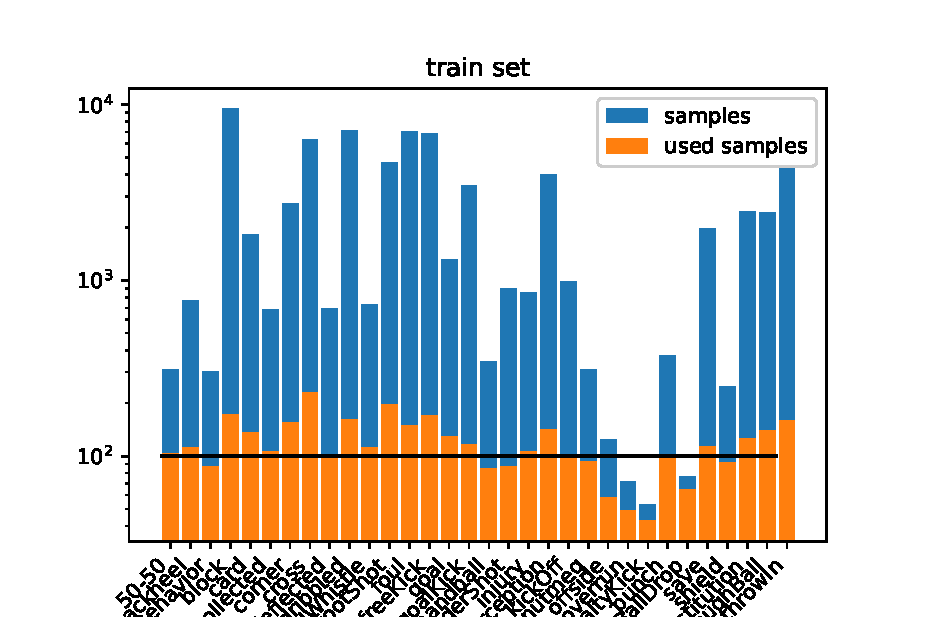
\includegraphics[width=.6\linewidth]{img/data-plots/4sec/class_distribution_used_samples_train_202010-1419-3803.eps}
    \caption{Beispielhaftes Resampling des Trainings-Sets (bei $\gls{tld:Delta} = 4.0$)}
    \label{fig:resamples}
\end{figure}

\subsection{Data Augmentation \& Standardisierung}
\label{subsec:data-augmentation}

Zu jeder Epoche werden je nach Batch-Größe mehrere Samples aus $D_{\text{train}}$, $D_\text{val}$ \bzw $D_\text{test}$ bestimmt.
Für jedes der Samples werden die jeweiligen Frames aus den Quellvideos dekodiert.

Data Augmentation beschreibt die Technik zusätzliche Trainingsdaten zu erlangen, indem zufällige Variationen gleicher Samples generiert werden (\cite{Gugger20}).
Durch den Einsatz der Temporal Augmentation wurden bereits zusätzliche Samples generiert, um Ungleichgewichtungen vorzubeugen, weshalb es keiner zusätzlichen Daten bedarf.
Jedoch können die Samples mit Methoden der gewöhnlichen Data Augmentation kombiniert werden um ein Overfitting auf teilweise (im Sinne von Überschneidungen) gleichen Samples zu verhindern.

Im Zuge der Data Augmentation wird jeder \gls{clip}, nachdem er dekodiert wurde, zunächst auf 90 \% seiner Höhe und Breite zufällig zugeschnitten.
Anschließend werden Helligkeit, Kontrast und Sättigung leicht verändert (Jittering; siehe~\cite{Tran18}).
In der Hälfte der Fälle wird das Bild horizontal gespiegelt.
Abschließend wird das Bild auf die Zielauflösung des jeweils verwendeten \gls{har}-Backbones verkleinert.
Für das Validierungs- und Testset wird nur ein 90 \%-iger zentraler Ausschnitt des Bildes erfasst und auf die Zielauflösung geschrumpft.
\autoref{fig:sample_example} zeigt ein beispielhaftes Sample nach Durchlaufen der Pre-Processing-Pipeline (bis einschließlich Data-Augmentation).

\begin{figure}
    \centering
    \includegraphics[width=.8\linewidth]{img/05_sample_example.png}
    \caption{Beispielhaftes Samples eines Eckstoßes bestehend aus 32 Frames}
    \label{fig:sample_example}
\end{figure}

Nach der Data Augmentation werden alle Tensoren standardisiert.
\Dh alle Samples werden auf einen Wertebereich von $\left[ -1, 1\right]$ projiziert -- mit einer Normalverteilung mit Mittelwert $\mu = 0$ und Standardabweichung $\sigma = 1$~\cite{Burkov19}.
Die Standardisierung erfolgt mit den Mittelwerten und Standardabweichung der vortrainierten Daten (\zB Kinetics) oder sofern nicht verfügbar mit den selbst ermittelten Werten des Datensets.
Anschließend werden die Werte auf den Bereich $\left[0, 1\right]$ normalisiert.

\chapter{Training}
\label{ch:training}

In diesem Kapitel wird der detaillierte Trainingsablauf mit all seinen Hyperparametern beschrieben.
Das Training stellt eine Form von Transfer Learning zur Multi-Label-Klassifikation dar.
Es werden ausschließlich vortrainierte Modell verwendet und angepasst.
Alle Rechenergebnisse basieren auf einem einheitlichen Trainingsprotokoll, welches es ermöglicht, die Ergebnisse zu vergleichen und zu reproduzieren.
%Die Implementationen basiert auf den Open-Source Bibliotheken PyTorch, Torchvision (für Bild- und Videoverarbeitung) und Ignite (als Framework für Training).

Dazu werden alle möglichen Hyperparameter aufgelistet, kategorisiert und eine Entscheidungsfindung für die Wahl erläutert.
Anschließend werden alle vorgelagerten Prozesse, der eigentliche Trainingsablauf, sowie nachgelagerte Prozesse veranschaulicht.

\begin{tcolorbox}[title=Todo]
    \begin{itemize}
        \item Wireframe: Relabel (Beispiel von Fehlerhaftem Sample)
    \end{itemize}
\end{tcolorbox}

Das Training von Deep-Learning-Modellen ist durch die Wahl etlicher Hyperparameter geprägt.
Einige können mithilfe gängiger Best Practices, andere durch manuelle Verfahren oder durch iteratives Ausprobieren bestimmt werden.
Der hier vorgestellte Trainingsablauf lässt sich in vier Parametergruppen gliedern:

\begin{description}
    \item[Sampling-Parameter] Die in \autoref{subsec:hyperparameter} vorgestellten Parameter $\gamma_s$ (Auflösung), $\gamma_\tau$ (Samplingrate) und $\gamma_t$ (Anzahl der Frames) sind Teil der Evaluation und werden in verschiedenen Experimenten ausprobiert.
    Der Richtwert $\gls{tld:Theta}_\text{train}$, der die Maximalzahl von Samples pro Klasse beschränkt, wird zunächst auf 100 gesetzt, in späterem Experimenten zur weiteren Optimierung jedoch erhöht.
    \item[Hardware-abhängige Parameter]
    Zu dieser Gruppe gehört \zB die Batch-Größe, die durch die Speicherkapazität der Grafikkarte beschränkt wird.
    In \autoref{subsec:hardwareeinschrankungen} wird der Umgang mit begrenzten Speicher beschrieben und wie die Parameter gewählt werden.
    \item[Modell-abhängige Parameter] Zu dieser Gruppe zählt vorrangig die zu wählende Lernrate, die bestimmt in welchem Maß die Modellparameter angepasst werden.
    Auch hierzu wird in \autoref{subsec:vorkehrungen} ein Verfahren zur Findung erläutert.
    \item[Sonstige Parameter] Alle übrigen Parameter werden auf der Grundlage vorherrschenden Best Practices oder den Implementationsdetails des jeweils vortrainierten Modells bestimmt.
\end{description}

\section{Vorbereitung}
\label{sec:vorbereitung}

Bevor das eigentliche Training startet, müssen Parameter wie Batch-Größe und Lernrate durch iterative Prozesse in jedem Experiment bestimmt werden.
Ebenfalls ist eine manuelle Einsicht in die Daten durch das Plotten zufälliger Samples (wie in \autoref{fig:sample_example}) hilfreich, um sicherzustellen, dass alle Pre-Processing-Schritte funktionieren.

\subsection{Hardwareeinschränkungen und Bestimmung der Batch Größe}
\label{subsec:hardwareeinschrankungen}

Die Experimente werden mithilfe einer einzelnen \gls{gpu} (Modell Tesla P100-PCIE-16GB \bzw Tesla V100-SXM2-16GB) durchgeführt.
Da die Feature-Maps proportional zu den Sampling-Parametern $\gamma_s$ und $\gamma_t$ wachsen, kann schon bei einer kleinen Batch-Größe das Speicherlimit der Grafikkarte erreicht werden.

Als Antwort auf diese Einschränkung werden zum einen die Modelle konsequent mit einer Genauigkeit von 16 Bit (Half Precision) statt der gängigen 32 Bit trainiert.
Zum anderen wird die Batch-Größe, als zentraler Parameter, der Einfluss auf Trainingsdauer und Performance hat, justiert.
Größere Batches liefern stabilere Gradienten und meist bessere Ergebnisse, verlangsamen jedoch das Training da mehr Epochen bis zur Konvergenz nötig sind (\cite{Gugger20}).
Als Richtwert wird eine Batch-Größe von 64 festgelegt.
Dieser Wert orientiert sich am Transfer Learning in~\cite{Feichtenhofer18} und stellt zugleich sicher, dass in jedem Update-Schritt potenziell alle 32 Klassen, sowie Background-Samples repräsentiert sein können.

Da eine Batch-Größe von 64 bei den allermeisten Experimenten nicht in den \gls{gpu}-Speicher passt, wird zunächst die maximal mögliche Batch-Größe mittels Binärer Suche bestimmt.
Ist die maximale Batch-Größe größer oder gleich dem Richtwert, wird der Richterwert als Batch-Größe übernommen.
Ist sie kleiner als der Richtwert, wird als weiteres Hilfsmittel eine Gradient Accumulation genutzt.
Diese stellt sicher, dass die Gradienten der kleinere Batches solange für den Backpropagation-Schritt aufsummiert werden bis der Richtwert von 64 Samples wieder erreicht ist.
Die eigentliche Batch-Größe wird dazu auf den größten gemeinsamen Teiler aus maximaler Batch-Größe und Richtwert abgerundet.
Sollte die maximale Batch-Größer die untere Grenze von 8 unterschreiten, muss in letzter Instanz auf das Training vorderer Layer verzichtet werden, um so zusätzlich Speicher zu sparen.
Die Auswahl über die Anzahl der Layer, die in diesem Fall eingefroren werden, passiert ebenfalls iterativ und wird entsprechend in den Experimenten angegeben.


\subsection{Bestimmung der Lernrate}
\label{subsec:vorkehrungen}

Für die Wahl der passenden Lernrate wird ein iterativer Test für verschiedenen Lernraten durchgeführt.
Der Test probiert verschiedene Lernraten aus und plottet diese gegen den resultierenden Fehler (in diesem Fall Binary Cross Entropy), wie \autoref{fig:lr-finder} zeigt.
Dabei wird diejenige Rate als Lernrate empfohlen, deren Abstieg maximal ist~\cite{Smith15}.

\begin{figure}
    \centering
    \bigimage{img/lr_finder}{0.65\textwidth}
    \caption{Lernraten-Finder mit markierter Empfehlung aus~\cite{Gugger20}}
    \label{fig:lr-finder}
\end{figure}

Da im Folgenden ausschließlich Transfer Learning angewandt wird, wird die Lernrate nicht als skalarer Wert, sondern ein Intervall definiert.
Mit sogenannte diskriminativen Lernraten (discriminative fine-tuning~\cite{Howard18}) erhalten vordere Layer eines Netzes kleinere Lernraten als hintere Layer.
Dem liegt die Idee zugrunde, dass die vortrainierten Low-Level-Features der vorderen Layer eine allgemeinere Gültigkeit haben und weniger an die neue Domäne angepasst werden müssen, als die High-Level-Features hinterer Layer.
Die diskriminativen Lernraten ergeben sich aus einem Intervall um den empfohlenen Richtwert, wobei das gesamte Intervall eine stetig negative Steigung ausweisen sollte.
Im Beispiel aus \autoref{fig:lr-finder} wäre $[1e^{-03}, 1e^{-01}]$ ein mögliches Interval.

\section{Trainingsablauf}
\label{sec:trainingsablauf}

Allen Experimenten geht die jeweilige Suche nach Batch-Größe und Lernraten voraus.
Anschließend findet das eigentliche Training nach einem wie folgt beschriebenen, fest definierten Ablauf statt.

\subsection{Trainingsschleife}
\label{subsec:trainingsschleife}

Alle Experimente folgen dem gleichen Schema in Form eines Trainings-Loops:
\autoref{fig:train-loop} zeigt den Algorithmus des Trainings-Loops, in der pro Epoche eine Schleife durchlaufen wird:

Zunächst werden Batches aus dem Trainingsset gesamplet, bevor der Vorwärts- und Rückwärts-Pass des \gls{har}-Modells durchlaufen wird.
Aus den Scores (Predictions) des Vorwärtspasses, werden mithilfe der Ground-Truth-Labels $y$ die Fehlerwerte (Losses) berechnet.
Scores und Losses werden intern zwischengespeichert und in einer separaten \code{Evaluator}-Komponente zwischengespeichert, die pro Epoche Metriken zur Bewertung des Modells erfasst und loggt.

Sobald alle Trainingsdaten einmal verarbeitet wurden, werden analog die Validierungsdaten gesamplet, die allerdings nur den Vorwärtspass des \gls{har}-Modells durchlaufen.
Diese resultierenden Scores und Losses werden analog im \code{Evaluator} zwischengespeichert.

Am Ende einer Epoche wird anhand der Metriken geprüft, ob das Modell overfittet.
Ist letzteres der Fall, kann der Trainings-Loop vorzeitig abgebrochen werden (Early-Stopping).

\begin{figure}[htbp!]
    \centering
    \bigimage{fig/training}{0.95\textwidth}
    \caption{Sequenzdiagramm: Trainings-Loop}
    \label{fig:train-loop}
\end{figure}

Nach dem Durchlauf werden alle Metriken, Hyperparameter, sowie die besten Modellgewichte (Checkpoints) und der Quellcode an einen persistenten Cloud-Speicher übermittelt, sodass keine Informationen verloren gehen.
Auch die Scores und Losses werden mit weiteren Daten zur Identifizierung der jeweiligen Samples in Form einer \gls{csv}-Datei übermittelt.
Die Speicherung von Scores und Losses dient letztlich der Fehleranalyse in \autoref{sec:nachgang}.

Zudem geht dem beschriebenen Ablauf der Schritt des Scheduling in jeder Trainingsiteration vorher.
Scheduling meint in diesem Zusammenhang das zeitabhängige Anpassen von Hyperparametern während des Trainings: in diesem Fall der Lernraten.

In allen Experimenten wird hierzu ein One-Cycle-Schedule~\cite{Smith15} erstellt, der die Lernraten in jedem Iterationsschritt anpasst.
Im ersten Drittel werden die Lernrate von einer 10x kleineren initial Lernrate aus angenähert, während sie sich in den letzten zwei Dritteln wieder auf null abkühlen.
\autoref{fig:one-cylce} zeigt einen exemplarischen Verlauf für die Basis-Lernrate von 0.01.
Diese Praxis verspricht eine schnellere Konvergenz, indem der Optimizer im ersten Drittel mehr Freiheitsgrade bekommt, um nach einem guten Startpunkt zu suchen und lokalen Minima zu entkommen.
In den hinteren Dritteln kann diese Startlösung langsamer optimiert werden als vorher, sodass zu große Sprünge vermieden werden.

\begin{figure}
    \centering
    \begin{subfigure}{.5\textwidth}
        \centering
        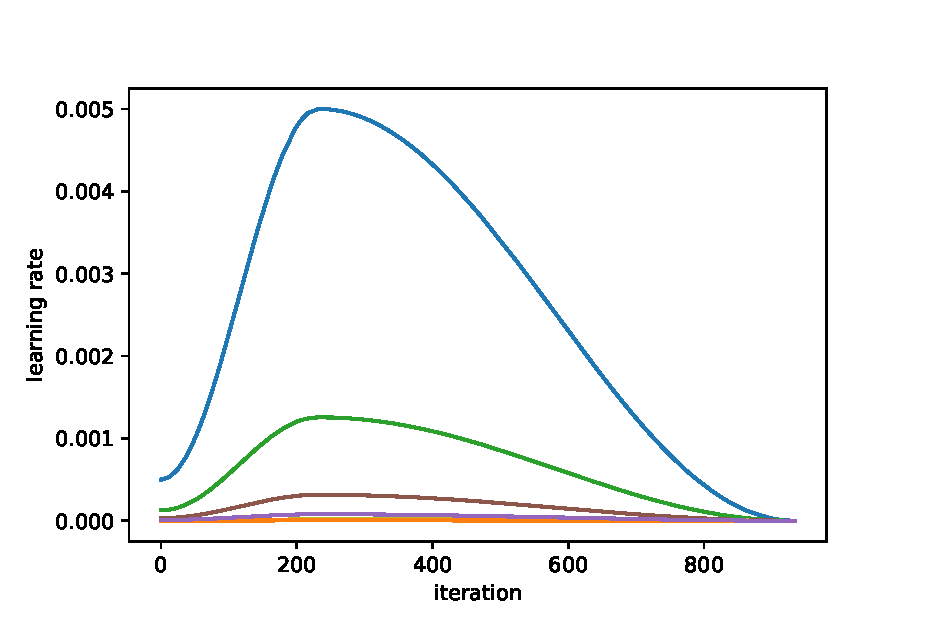
\includegraphics[width=.9\linewidth]{img/06_one_cycle_lin.eps}
        \caption{lineare Skala}
    \end{subfigure}%
    \begin{subfigure}{.5\textwidth}
        \centering
        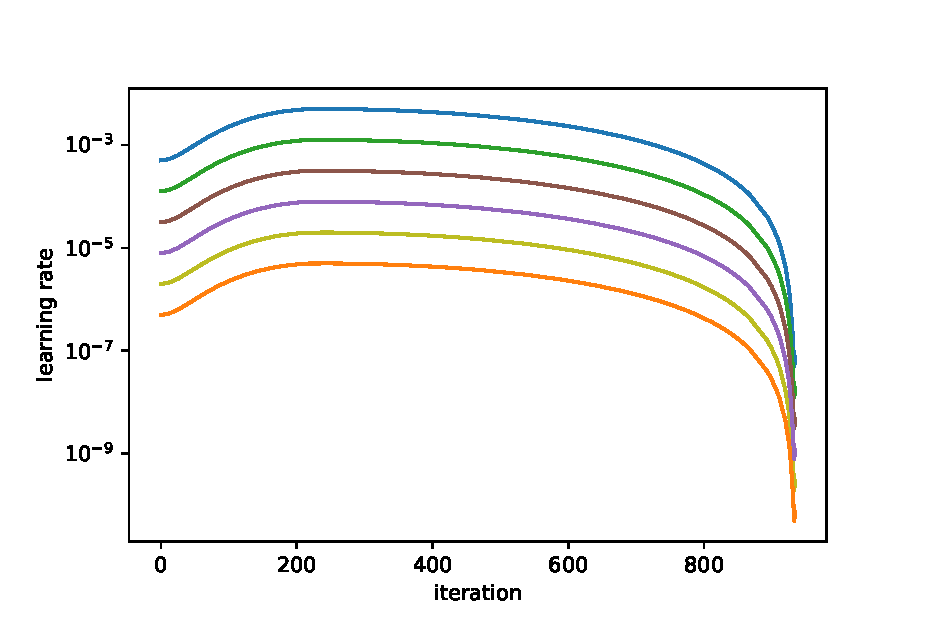
\includegraphics[width=.9\linewidth]{img/06_one_cycle_log.eps}
        \caption{logarithmische Skala}
    \end{subfigure}
    \caption{One Cycle Schedule für diskriminativen Lernraten}
    \label{fig:one-cylce}
\end{figure}

Der Backward-Pass basiert auf einem Adam-Optimierer~\cite{Kingma14} mit der Standardkonfiguration nach~\cite{Gugger20}.
Die Anzahl der Epochen wird in der ersten auf 10 beschränkt, was zum Initialisieren und einen einfachen Benchmark ausreicht.
In späteren Experimenten werden meist weniger Epochen verwendet, da das Modell bereits auf ähnliche Daten angepasst ist.

\subsection{Reaktive Änderungen}
\label{subsec:reaktive-aenderungen}

Wie schnell das Modell innerhalb des Trainings-Loops lernen kann ist letztlich auch von der Architektur selbst abhängig.
Die Zykluslänge im One-Cycle-Scheduling ist definiert durch die Anzahl der Epochen.
Sollte ein Modell im Zuge des Trainings massiv overfitten, ist es oft hilfreich den Durchlauf neu zu starten und dabei die Zahl der Epochen auf diejenige Epoch zu beschränken, in der zuvor das Overfitting begann~\cite{Gugger20}.

Eine weitere Reaktion ist der Einsatz von L2-Regularisierung, die die Summe der Modellparameter in die Fehlerfunktion einfließen lässt.
Das Maß des Einflusses wird durch eine Weight-Decay-Rate bestimmt, die, sofern nicht anders hervorgehoben, immer aus den Hyperparametern des vortrainierten Modells übernommen wird.

\subsection{Metriken}
\label{subsec:metriken}

Die in jeder Epoche erhobenen Metriken geben Aufschluss darüber, wie gut das aktuelle Modell auf dem jeweiligen Datenset performt und wie sich die Performance zeitlich entwickelt.
Während des Trainings werden folgende globalen Metriken erfasst:

\begin{itemize}
    \item Balanced Accuracy: $BA = \frac{1}{2} ( \frac{TP}{TP + FN} + \frac{TN}{FP + TN} )$
    \item Precision: $PR = \frac{TP}{TP+FP}$
    \item Recall: $RE = \frac{TP}{TP+FN}$
    \item F1-Score: $F1 = \frac{2 \cdot TP}{2 \cdot TP + FP + FN}$
    \item Area Under the Receiver Operating Characteristic Curve (AUROC)
\end{itemize}

Die oberen vier Metriken, werden jeweils pro Klasse erhoben, um später Aussagen über die individuelle Lernbarkeit einer einzelnen Klasse treffen zu können.
Darüber hinaus wird der Durchschnitt über alle Klassen Klasse (macro) oder das direkte Verhältnis auf Basis der klassenübergreifend aufsummieren Faktoren (TP, FP, etc.) erfasst (micro).
Sofern nicht anders hervorgehoben, sind die im weiteren Verlauf vorgestellten, skalaren Metrikwerte immer Macro-Werte.

\section{Verifikation}
\label{sec:nachgang}

Im Phase 3 der Experimente werden basierend auf den vorhergegangenen Experimenten potenzielle Daten-Fehler verifiziert.
Da aus Zeitgründen nicht alle Samples kontrolliert werden können, wird sich auf diejenigen Samples beschränkt, die mit erhöhter Wahrscheinlichkeit fehlerhaft gelabelt sind.
Hierfür wird auf die während des Trainings persistierten Scores und Losses zurückgegriffen, die in einem Fehlerbericht persistiert sind.
Mithilfe des Fehlerberichts genügt es, nur die Samples mit den höchsten Loss-Werten manuell zu kontrollieren.

Schon während des Samplings (\autoref{subsec:segmentierung-und-sampling-strategie}) wird jedes Sample mit einer eindeutigen ID verknüpft, die sich aus dem zugehörigen Match und der Startmarkierung (in Videozeit) zusammensetzt.
Mithilfe der ID können die \gls{annotationen} auch nachträglich aus der JSON-Datenbank geladen und die Scores mit den Ground-Truth-Labels des Samples verglichen werden.
Dabei werden die Samples der besten Epoche für alle Datensets absteigend nach ihrem Loss sortiert und mithilfe eines Relabel-Tools verifiziert und im Fehlerfall \ggf korrigiert.
Wird ein Fehler entdeckt kann dieser auf dreierlei Weisen behoben werden:

\begin{description}
    \item[Zusätzliche Aktion] Eine Aktion, die in den \gls{annotationen} vorher nicht erfasst war, ereignet sich im Videobild.
    Die Aktion kann als Tupel, bestehend aus Label und Zeitfenster, der Datenbank hinzugefügt werden.
    Dieser Fall tritt \zB auf, wenn eine Wiederholung gezeigt wird.
    \item[Verschobene Aktion] Eine Aktion, tritt im Videobild früher oder später auf, als es in den Ground-Truth-Daten dokumentiert ist.
    In der Datenbank findet sich genau die gesuchte Aktion, deren Zeitfenster jedoch nicht übereinstimmt.
    In diesem Fall kann die \code{segment}-Eigenschaft der Annotation in der Datenbank geändert werden.
    \item[Verdeckte Aktion] Eine Aktion, die stattgefunden hat, ist im Kamerabild nicht zu sehen und muss aus der Datenbank gelöscht werden.
\end{description}

Das Relabel-Tool speichert die Änderungen nicht direkt in der JSON-Datenbank, sondern in einer zusätzlichen Datenstruktur, die ausschließlich die Datenbank-Transaktionen enthält, die für ein Update notwendig sind.
Zur Laufzeit wird die JSON-Datenbank in den Arbeitsspeicher geladen und kann dort optional mithilfe der Transaktionsdatei angepasst werden.
Um die Transaktionen endgültig zu speichern, kann die angepasste Datenbank mit einer neuen Versionsnummer wieder auf dem Dateisystem persistiert werden.

Die Verifikation folgt einem definiertem Protokoll:
Sind alle Experimente einer Phase abgeschlossen, wird zunächst eine neue Transaktionsdatei erstellt.
Für jedes der Experimente wird das Relabel-Tool mit den persistierten Score- und Loss-Werte des Fehlerreports initialisiert.
Das Relabel-Tool erhält ebenfalls Zugriff auf die bestehende JSON-Datenbank.
Die Samples werden absteigend nach Loss-Wert sortiert und dem Nutzer interaktiv präsentiert.
Der Nutzer kann die einzelnen zugrunde liegenden \gls{annotationen} eines Samples ändern oder löschen oder eine neue Annotation hinzufügen.
Jede dieser drei Operationen lässt sich in Form einer Transaktion in einer \gls{csv}-Datei speichern.
Nach der Verifikation eines Experiments werden die Transaktionen separat gespeichert, dann auf die Datenbank angewendet und dann die Datenbank in einer neuen Version gespeichert.
Die geänderten \gls{annotationen} werden zudem als verifiziert in der Datenbank markiert, sodass der Nutzer die gleichen Fehler nicht mehrmals im Relabel-Tool vorgeschlagen bekommt.

Eine weitere Funktion des Fehlerreports besteht darin nach Auffälligkeiten in den Daten zu suchen:
Es kann der durchschnittliche Fehler pro Video ermittelt werden und Ausreißer können mit einem z-Test identifiziert werden.
Diese Ausreißer sind \zB Videos mit vielen Kodierungsfehlern oder einer nicht konstanten Abspielgeschwindigkeit, die im Rahmen dieser Arbeit nicht zum Einsatz kommen sollten, da sie die Qualität des Datensets im Allgemeinen beeinträchtigen.
Falls die Qualität dieser Videos inakzeptabel ist, werden sie manuell aus der Datenbank entfernt.

\chapter{Ergebnisse}
\label{ch:results}

In diesem Kapitel werden die Ergebnisse der in \autoref{sec:experimente} beschriebenen Experimente vorgestellt.
Die Evaluation schließt die Ergebnisse aller vier Phasen, häufige Fehler in der Verifikation, sowie eine grobe Kategorisierung der Aktionsklassen ein.

\section{Benchmark}
\label{sec:benchmark}

In diesem Abschnitt werden die Rechenergebnisse der verschiedenen Modelle miteinander verglichen.
Als Baseline-Modelle wurden R2+1D-34, ir-CSN-152 und zwei Varianten von SlowFast-50 getestet, die mit $\gls{tld:Theta}_\text{train} = 200$ für 10 Epochen trainiert.
Beide SlowFast-Varianten wurden zunächst ohne Hinzunahme von Non-Local-Blöcken trainiert.
In \autoref{tab:phase1} sind die Ergebnisse zu sehen, wobei alle Hyperparameter aus den ursprünglichen Publikationen übernommen wurden.
Die Metriken basieren auf einem einheitlichen Testset mit $\Delta_\text{test} = 3$.
Der Zeitkontext im Testset ist damit größer als im Trainingsset und wird durch zusätzliche Frames erreicht (\zB 36 statt 32 Frames bei ir-CSN), die die Modelle durch ihr dynamisches Pooling wieder auf die passende Länge stauchen.

Überraschend ist, dass die SlowFast-Variante mit $\alpha = 8$ (SlowFast-50-4x16) bessere Ergebnisse erzielt als die Variante mit $\alpha = 4$ (SlowFast-50-8x8).
Im ersteren erhält der Slow-Pathway schließlich nur halb so viele Frames, wie im letzteren und kann sich damit noch mehr auf räumliche Features fokussieren.
Da die Ergebnisse für SlowFast-50-4x16 durchweg besser ausfallen, wird diese Variante im weiteren Verlauf als SlowFast-Baseline-Modell bezeichnet.

\begin{figure}
    \centering
    \small
    \csvreader[no head,tabular=|l|r||r|r|r|r|,
    table head=\hline,late after line=\\\hline]{tbl/exp_phase_1.csv}
    {1=\model,2=\aurocval,3=\baval,4=\fbetaval,5=\lr,6=\bs,7=\ba,8=\rec,9=\prec,10=\auroc}
    {\model & \lr & \ba & \prec & \rec & \auroc}
    \caption{Ergebnisse aus Benchmark}
    \label{tab:phase1}
\end{figure}

\subsection{Vergleich der Modelle}
\label{subsec:vergleich-der-modelle}

Vergleicht man die Ergebnisse, fällt auf, dass ir-CSN die besten und R2+1D die schwächsten Metriken vorweist.
Damit einher geht allerdings auch ein größerer Fußabdruck:
während bei R2+1D (\bzw SlowFast) eine maximale Batch-Größe von 24 (\bzw 21) möglich war, erlaubt ir-CSN nur eine Batch-Größe von maximal 5 bei gleicher Speicherauslastung.
Dennoch wird für den weiteren Verlauf ir-CSN als einziges Baseline-Modell weitergeführt.
Die weitere Optimierung der anderen Modelle wird aus Zeitgründen nicht weiter verfolgt.

\subsection{Verifikation}
\label{sec:verifikation}

Im nächsten Schritt werden die Fehler der Experimente genauer analysiert.
Grundlage sind die drei Baseline-Modelle aus der ersten Phase.
Im Zuge der Analyse werden innerhalb einer statistischen Analyse Auffälligkeiten im Fehlerreport analysiert.
Zusätzlich werden jeweils 50 der Samples mit den größten Fehlerwerten innerhalb eines Experiments verifiziert.

Bei der statistischen Analyse werden die Samples nach Halbzeitvideo gruppiert und der Mittelwert der Fehler wird berechnet.
Dadurch konnten insgesamt vier fehlerhafte Videos erkannt werden, da diese auffällig hohe Mittelwerte hatten (mit einem z-Score über 3).
Zudem wurde für zwei weitere Videos, die nach dem gleichen Kriterium aufgefallen sind, das manuelle Aligning nachjustiert.

Bei der Verifikation einzelner Samples wurden pro Modell 50 Samples (im Verhältnis 3:1:1 je Datensubset) mit den höchsten Fehlerwerten manuell verifiziert.
Dies entspricht 150 Samples, bei denen insgesamt 267 Transaktionen mit Korrekturvorschlägen gespeichert wurden.
Die Transaktionen bestehen zu 72.6 \% aus Zeitfensteranpassungen.
22.8 \% sind Löschungen von nicht sichtbaren Aktionen und 4.5 \% sind hinzugefügte Aktionen.
Die häufigsten Klassen für Zeitfensteranpassungen sind \code{save} (32), \code{footShot} (30), \code{cross} (14) und \code{card} (10).
Besonders auffällig ist, dass \zB \code{save}- oder \code{card}-Aktionen in den Stammdaten, teils mehrere Sekunden, zu früh auftreten.
Nach Durchsicht der Daten werden die 267 Transaktionen in die Datenbank übernommen.
Alle weiteren Experimente beziehen sich somit auf die korrigierte Datenbank.

Eine weitere Optimierung des Baseline-Modells (ir-CSN) anhand der verifizierten Datenbank, führt zu einer zusätzlichen Steigerung der Balanced Accuracy von 1.5 \% Prozent (siehe \autoref{tab:phase1}).

\section{Hyperparameter-Optimierung}
\label{sec:hyperparameter-optimierung}

Das aktuelle Baseline-Modell bilden in seiner ursprünglichen Form mit $T=32$ und $\tau = 2$ einen Zeitkontext von 2.67 Sekunden ab.
Da diese Hyperparameter auf Grundlage eines anderen Datensets festgesetzt wurden, werden die oben genannten Hyperparameter im nachfolgenden Experiment in einer Grid-Suche anhand des vorliegenden Datensets angepasst.
Das Vorgehen ist weiter motiviert durch die Mindest-Dauer von 4 Sekunden in SoccerDB \bzw der unteren Grenze von 3 Sekunden basierend auf \gls{sbod}.

Alle Modelle nutzen eine dynamisches Avg-\pool-Layer zwischen dem letzten \conv- und dem ersten \fc-Layer, das die Verarbeitung von \glspl{clip} variabler Länge $T$ zulässt.
Um eine geeignete Methode zu finden, wird der Einfluss des Avg-Poolings durch ein höheres $T$ und von schnelleren \glspl{clip} durch einen höheren Zeitschritt $\tau$ verglichen.
Die Grid-Suche betrachtet also Punkte für verschiedene Werte von $T$ und $\tau$, wobei der dadurch beeinflusste Zeitkontext sich innerhalb der unteren und oberen Grenze von 3 \bzw 6 Sekunden bewegen soll.
Für die Wahl von $T$ werden sechs Werte zwischen 24 und 64 getestet, wobei 64 die maximale Anzahl von Frames darstellt.
Zusätzliche Frames würden die Kapazität der \gls{gpu} überschreiten und sind im Rahmen der Arbeit technisch nicht möglich.
Die Punkte für $\tau$ werden so gewählt, dass sich der resultierende Zeitkontext etwas um eine Sekunde unterscheidet.
Zusätzlich wird das Baseline-Modell der vorherigen Phase erneut getestet.
\autoref{fig:exp-hparams-grid} zeigt alle getesteten Punkte der Grid-Suche, sowie Orientierungslinien für den Zeitkontext.

\begin{figure}
    \centering
    \begin{subfigure}{.25\textwidth}
        \centering
        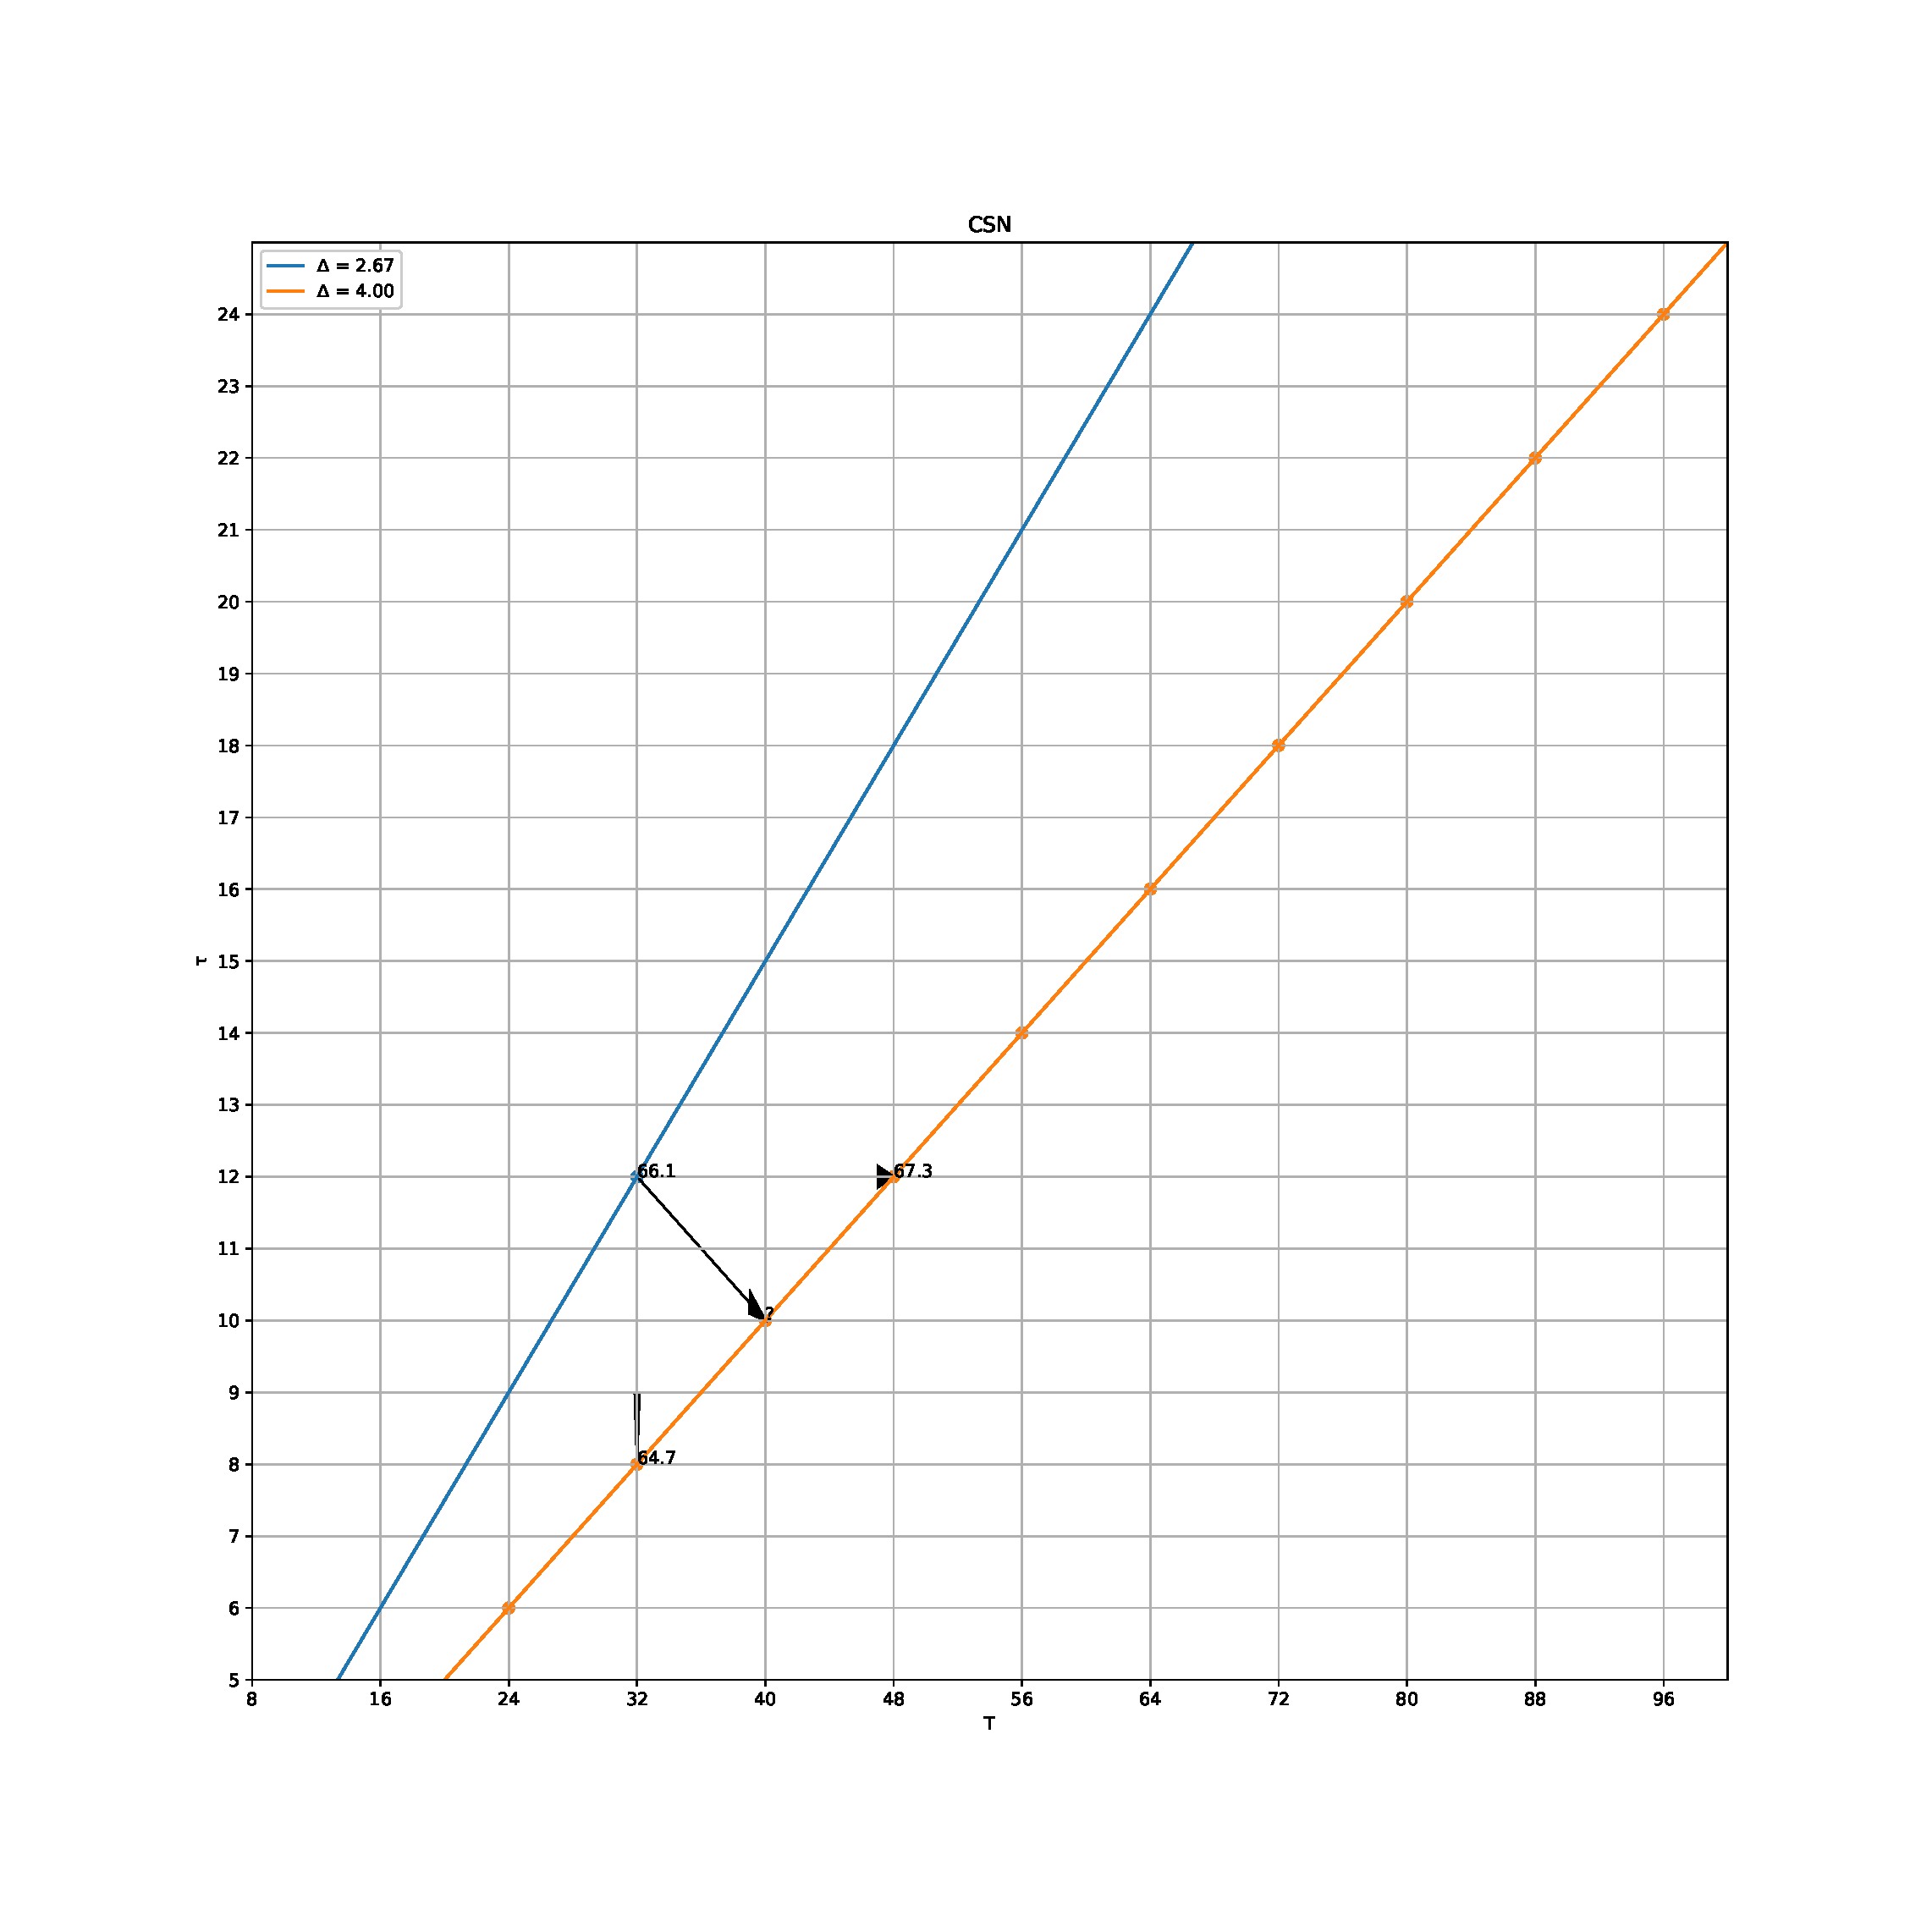
\includegraphics[width=0.99\textwidth, keepaspectratio, interpolate]{img/07_grid_csn.eps}
        \caption{Punkte für Grid-Suche}
        \label{fig:exp-hparams-grid}
    \end{subfigure}%
    \begin{subfigure}{.35\textwidth}
        \centering
        \includegraphics[width=0.99\textwidth, keepaspectratio, interpolate]{img/07_par_cor_prec.eps}
        \caption{Precision für Grid-Suche}
        \label{fig:exp-hparams-prec}
    \end{subfigure}
    \begin{subfigure}{.35\textwidth}
        \centering
        \includegraphics[width=0.99\textwidth, keepaspectratio, interpolate]{img/07_par_cor_rec.eps}
        \caption{Recall für Grid-Suche}
        \label{fig:exp-hparams-rec}
    \end{subfigure}
\end{figure}

Aufgrund der Vielzahl zusätzlicher Experimente wird die Laufzeit bei diesen Experimenten durch $\gls{tld:Theta}_\text{train} = 100$ und auf 3 Epochen begrenzt.
Da das Baseline-Modell nach der ersten Phase bereits neue Feature gelernt hat, wird zu Beginn eine neue Lernrate gesucht, die für alle Trainings der Grid-Suche gilt und dem Intervall $[3e^{-4}, 3e^{-6}]$ entspricht.
\autoref{fig:exp-hparams-prec} und \autoref{fig:exp-hparams-rec} veranschaulichen die Ergebnisse der Grid-Suche in Form von Parallelen Koordinaten.
Es fällt auf, dass die Hyperparameter sehr gegensätzlichen Einfluss auf die Metriken Precision und Recall haben.
So wirken sich zusätzliche Frames und ein hoher oder gleichbleibender Zeitschritt positiv auf den Recall aus, während sich beides eher negativ auf die Precision auswirkt.
Ein erhöhter Zeitkontext wirkt sich ebenfalls positiv auf den Recall auf.
Die Precision scheint hingegen unabhängig vom Zeitkontext zu sein.

\begin{figure}
    \centering
    \small
    \csvreader[no head,tabular=|r|r|r||r|r|r|,
    table head=\hline,late after line=\\\hline]{tbl/exp_phase_2.csv}
    {1=\model,2=\s,3=\t,4=\sr,5=\d,6=\auroc,7=\ba,8=\fone}
    {\t & \sr & \d & \ba & \fone & \auroc}
    \caption{Ergebnisse des Validierungssets aus Phase 2}
    \label{tab:phase2}
\end{figure}

Um ein gutes Gleichgewicht zwischen den beiden Metriken zu erlangen, werden nachfolgend nur noch Ergebnisse betrachtet, die einen besonders hohen F1-Score aufweisen.
In \autoref{tab:phase2} sind nur Experimente gelistet, die maximal 1 \% von dem maximale F1-Score abweichen.
Als zusätzlicher Filter werden Experimente ausgeschlossen, deren Balanced Accuracy mehr als 1 \% vom Maximum abweicht.
Als Baseline-Modell für die nachfolgenden Experimente wird die Konfiguration mit $T=48$ und $\tau=2.4$ (10 \gls{fps}) gewählt.
Da sich für dieses Modell ein Zeitkontext von $\Delta_\text{fit} = 4.8$ ergibt, wird für dieses und alle folgenden Experimente ein zweites Testset gesamplet mit $\Delta_\text{test} = 5$.
Das neue Baseline-Modell wird erneut für 5 Epochen mit $\gls{tld:Theta}_\text{train} = 200$ trainiert und liefert dabei eine Balanced Accuracy von 68.18~\% auf dem neuen Testset.

\section{Kategorisierung der Aktionsklassen}
\label{sec:kategorisierung-der-aktionsklassen}

In den bisherigen Experimenten wurden jeweils nur die durchschnittlichen Metriken (macro) über alle Klassen betrachtet.
In diesem Abschnitt wird das Baseline-Modell der zweiten Phase erstmals pro Klasse evaluiert.
Dabei werden besonders schwere Klassen aus dem Datenset entfernt und das Modell wird ohne diese Klassen erneut nachtrainiert.

Zuerst werden die Metriken des vorangegangenen Experiments pro Klasse erhoben.
\autoref{fig:ba_by_class} zeigt die Balanced Accuracy zum Baseline-Modell aus Phase 2.
Dem ist entnehmen, dass es teils sehr starke Abweichungen innerhalb der verschiedenen Klassen gibt.
Während Aktionen wie \code{corner}, \code{footShot} oder \code{throwIn} hohe Werte vorweisen, können andere Klassen wie \code{offside} oder \code{handball} fast gar nicht klassifizieren werden.

%Das wird insbesondere deutlich wenn man die Metriken Precision und Recall in \autoref{fig:precision-recall} betrachtet.

\begin{figure}
    \centering
    \begin{subfigure}{.24\textwidth}
        \centering
        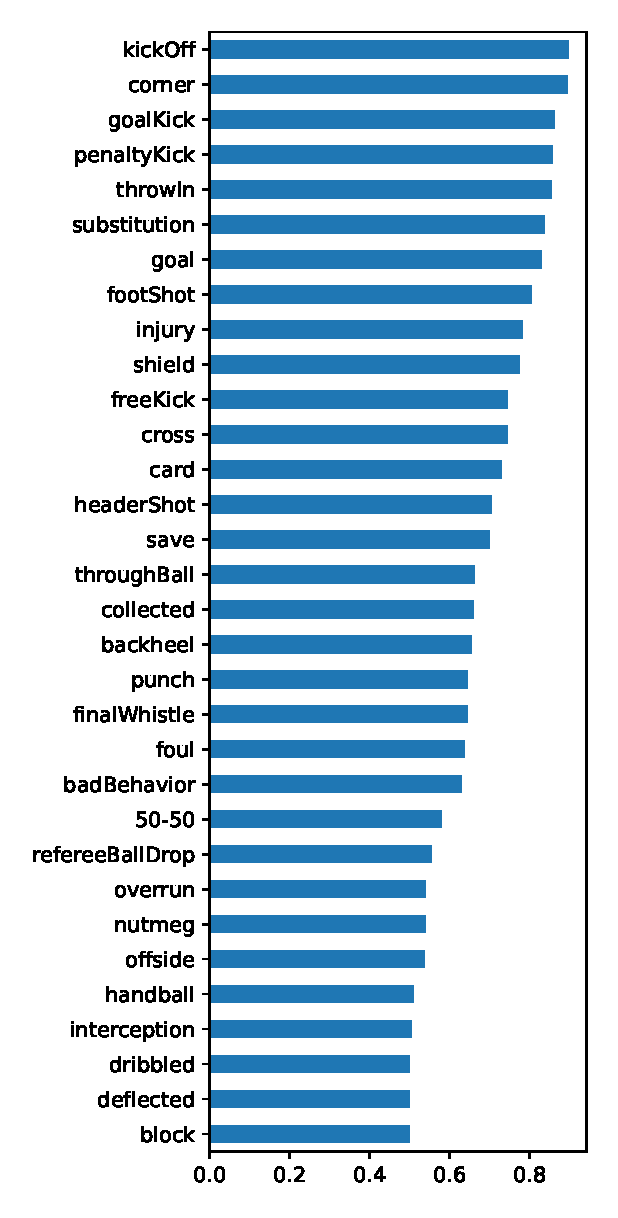
\includegraphics[width=0.99\textwidth, keepaspectratio, interpolate]{img/07_ba_by_class_ph_2.eps}
        \caption{Balanced Accurcy \newline mit 32 Klassen}
        \label{fig:ba_by_class}
    \end{subfigure}%
    \begin{subfigure}{.24\textwidth}
        \centering
        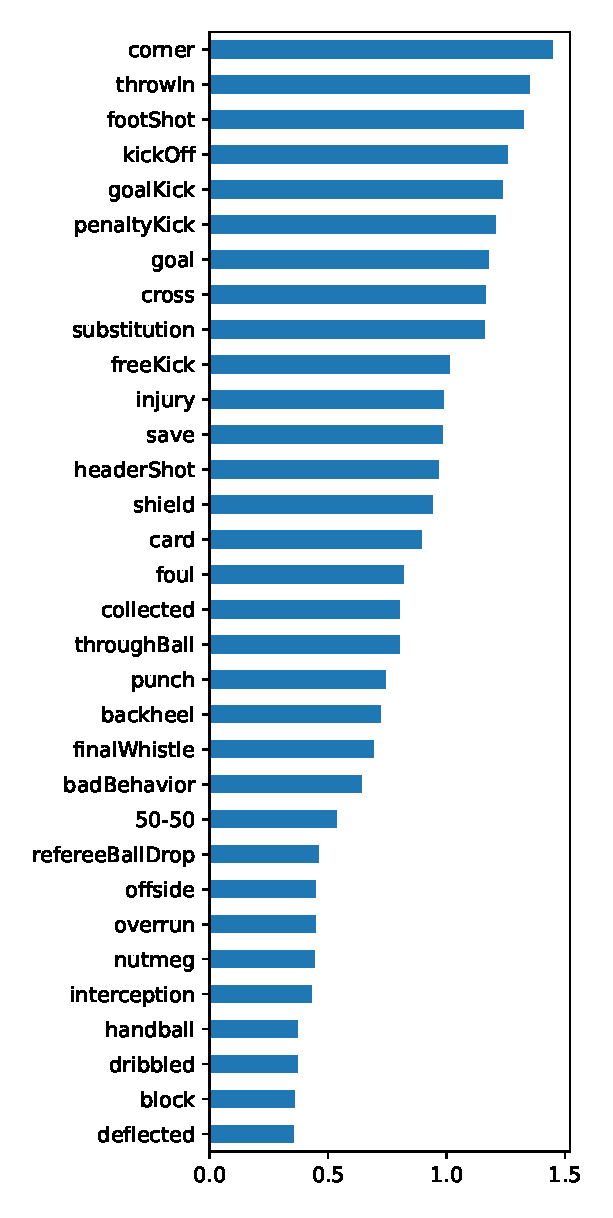
\includegraphics[width=0.99\textwidth, keepaspectratio, interpolate]{img/07_pca_by_class_ph_2.eps}
        \caption{PCA-0 \newline mit 32 Klassen}
        \label{fig:pca_by_class_phase_2}
    \end{subfigure}
    \begin{subfigure}{.24\textwidth}
        \centering
        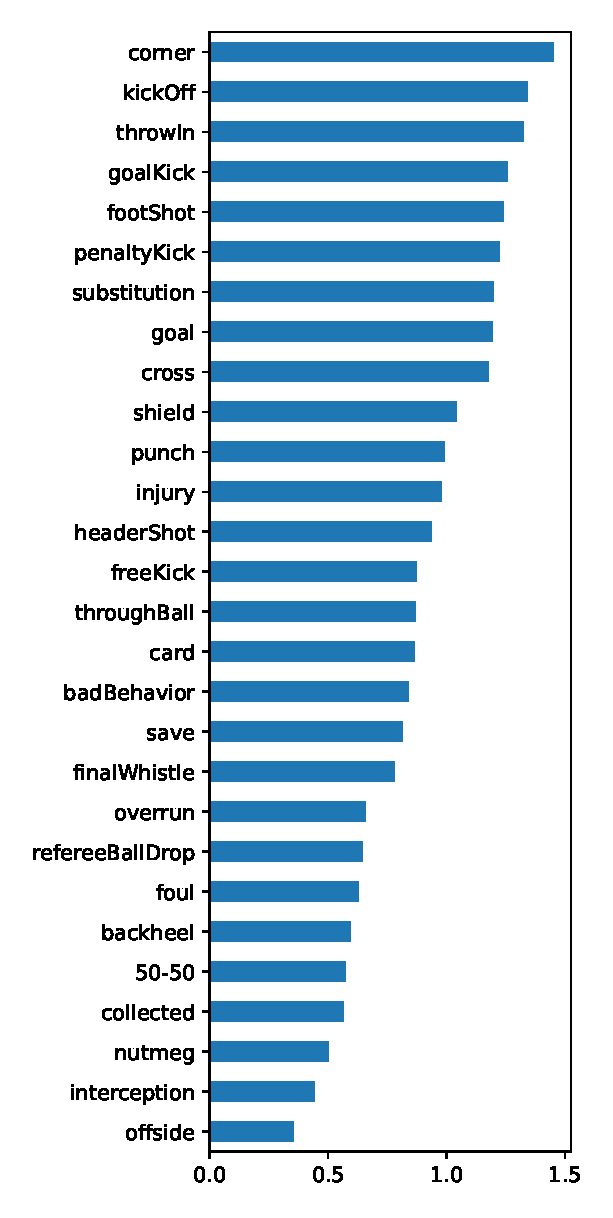
\includegraphics[width=0.99\textwidth, keepaspectratio, interpolate]{img/07_pca_by_class_socc_har_28.eps}
        \caption{PCA-0 \newline mit 28 Klassen}
    \end{subfigure}
    \begin{subfigure}{.24\textwidth}
        \centering
        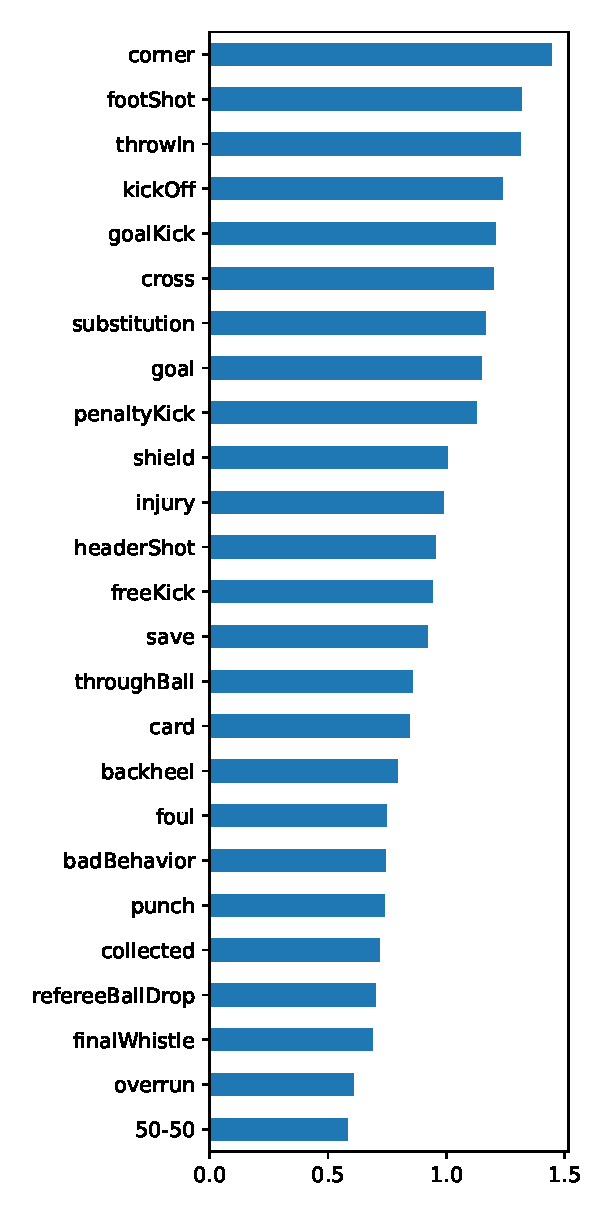
\includegraphics[width=0.99\textwidth, keepaspectratio, interpolate]{img/07_pca_by_class_socc_har_25.eps}
        \caption{PCA-0 \newline mit 25 Klassen}
        \label{fig:pca_by_class_phase_3}
    \end{subfigure}
    \caption{Metriken pro Klasse}
    \label{fig:class-metrics}
\end{figure}

%Dabei fällt auch auf, dass vor die Klassen im unteren Bereich mit einer niedrigen Precision viele False Positives verursachen, obwohl sie zum Teil einen hohen Recall haben.
%Auffällig ist auch, dass Aktionen, die sich im laufenden Spiel ereignen (\code{foul}, \code{cross}, \code{footShot}, \code{save}) einen besonders hohen Recall haben, während Aktionen die oft mit Spielunterbrechungen und Nahaufnahmen einhergehen (\code{substitution}, \code{goal}, \code{injury}) einen sehr niedrigen Recall aufweisen.

Da sich für jede erhobene Metrik eine abweichende Rangfolge der Klassen ergibt, ist es schwierig auf eine allgemeingültige Rangordnung abzubilden, die die Komplexität der Klassen widerspiegelt.
Es kann also keine pauschale Aussage über die Schwierigkeit einer Aktionsklassen gemacht werden.
Dennoch lässt sich anhand der erfassten Metriken eine grobe Ordnung erstellen, auch wenn sie allgemein nicht repräsentativ ist.
Hierzu werden alle fünf Metriken pro Klasse zu einer zweidimensionalen Matrix $M \in \mathbb{R}^{(A \times 5)}$ angeordnet und im Zuge einer \gls{pca} auf einen eindimensionalen Vektor projiziert.
Die erste Komponente der \gls{pca} $c_0 \in \mathbb{R}^{(5 \times 1)}$ deckt mit 80 \% hinreichend viel Varianz ab und projiziert die Metriken auf einen Vektor:

\begin{equation}
    \label{eq:pca}
    \text{pca}_0 = M \cdot c_0
\end{equation}

Die resultierende Rangordnung ist in \autoref{fig:pca_by_class_phase_2} abgebildet.
Als Folge werden die schwächsten vier Klassen aus dem ursprünglichen Datenset entfernt und das Modell wird erneut mit den übrigen 28 Klassen und $\gls{tld:Theta}_\text{train} = 300$ nachtrainiert.
Anschließend wird dieser Prozess erneut wiederholt, indem drei weitere Klassen entfernt werden und das Modell nur mit den 25 besten Klassen nachtrainier wird.
Nach beiden Trainings wurden wieder jeweils 50 Sample verifiziert und dabei insgesamt 187 weitere Transaktionen vorgenommen, um die Datenqualität zu verbessern.

Durch das Ausschließen dieser besonders schweren Klassen konnte eine zusätzliche Steigerung der Balanced Accuracy von 2.4~\% \bzw 6.4~\% erwirkt werden.
Das Modell mit 25 Klassen gilt fortan als Baseline-Modell der dritten Phase und \autoref{fig:pca_by_class_phase_3} zeigt die resultierende Ordnung der Klassen nach ihrer Schwierigkeit.
Analysiert man die Ordnungen, fällt auf, dass vor allem Klassen, die einen hohen Detailgrad in der Erkennung erfordern (\code{nutmeg}, \code{handBall}, \code{deflected}) schlecht abschneiden.
Eine mögliche Erklärung ist die geringe Auflösung der Modelle, die nicht alle Informationen abbilden kann.
Das Gegenteil ist der Fall bei Klassen, die oft in Kombination mit Nahaufnahmen gezeigt werden, wie \code{injury} oder \code{substitution}.
Ebenfalls schlecht schneiden Klassen ab, die eine hohe Kontextabhängigkeit haben, wie \code{offside} oder \code{finalWhistle}.
Während Klassen, die durch räumliche Gegebenheiten (insbesondere der Spielfeldmarkierungen) geprägt sind (\code{kickOff}, \code{corner}, \code{throwIn}), deutlich besser abschneiden.

\subsection{Vergleich zu bestehenden Datensets}
\label{subsec:evaluation-auf-teilmengen}

Aufgrund des zeitlichen Rahmens dieser Arbeit war es nicht möglich einen direkten Vergleich des Baseline-Modells anhand der Original-Datensets von SoccerNet und SoccerDB durchzuführen.
Für eine grobe Einordnung wurden jedoch zwei weitere Untermengen von SOCC-HAR-32 abgeleitet -- mit den gleichen Aktionsklassen aus den genannten Datensets.
Das Baseline-Modell dieser Phase wurde anhand beider Subsets ohne weiteres Training evaluiert.
Die Ergebnisse in \autoref{tab:eval_subset} sind also keinesfalls direkt vergleichbar oder repräsentativ, da die Datengrundlage eine andere ist.
Es soll dem Leser jedoch eine grobe Einordnung ermöglichen.

\begin{figure}
    \centering
    \small
    \csvreader[no head,tabular=|l||r|r|r|,
    table head=\hline,late after line=\\\hline]{tbl/eval_subsets.csv}
    {1=\dataset,2=\ba,3=\fbeta,4=\auroc}
    {\dataset & \ba & \fbeta & \auroc}
    \caption{Evaluation auf Teilmengen von Aktionsklassen}
    \label{tab:eval_subset}
\end{figure}

\section{Training mit erhöhter Auflösung}
\label{sec:fine-tuning}

\begin{tcolorbox}[title=WIP]
    \begin{itemize}
        \item Werte nachtragen
    \end{itemize}
\end{tcolorbox}

In der vierten Phase wird das Baseline-Modell der dritten Phase mit einer höheren Auflösung $S$ nachtrainiert.
Das Vorgehen, welches sich am in~\cite{Wu20} vorgestellten Multi-Grid-Training orientiert, erhöht die Auflösung alle 5 Epochen.
So findet ein zusätzliches Experiment statt mit $S=240$ und eins mit $S=256$.
Eine höhere Auflösung ist aufgrund der Hardware-Einschränkungen nicht möglich.
\autoref{tab:exp4} zeigt die Ergebnisse dieser und aller vorangegangenen Phase im Vergleich.

\begin{figure}
    \centering
    \small
    \csvreader[no head,tabular=|l|l|r|r||r|r|r||r|r|r|,
    table head=\hline,late after line=\\\hline]{tbl/exp_phase_1-4.csv}
    {1=\phase,2=\s,3=\t,4=\lilTau,5=\bigDelta,6=\auroc,7=\ba,8=\fbeta,9=\bigTheta,10=\socchar}
    {\phase & \socchar & \bigTheta & \bigDelta & \s & \t & \lilTau & \ba & \fbeta & \auroc}
    \caption{Ergebnisse aus Phase 1-4}
    \label{tab:exp4}
\end{figure}

%\begin{figure}
%    \centering
%    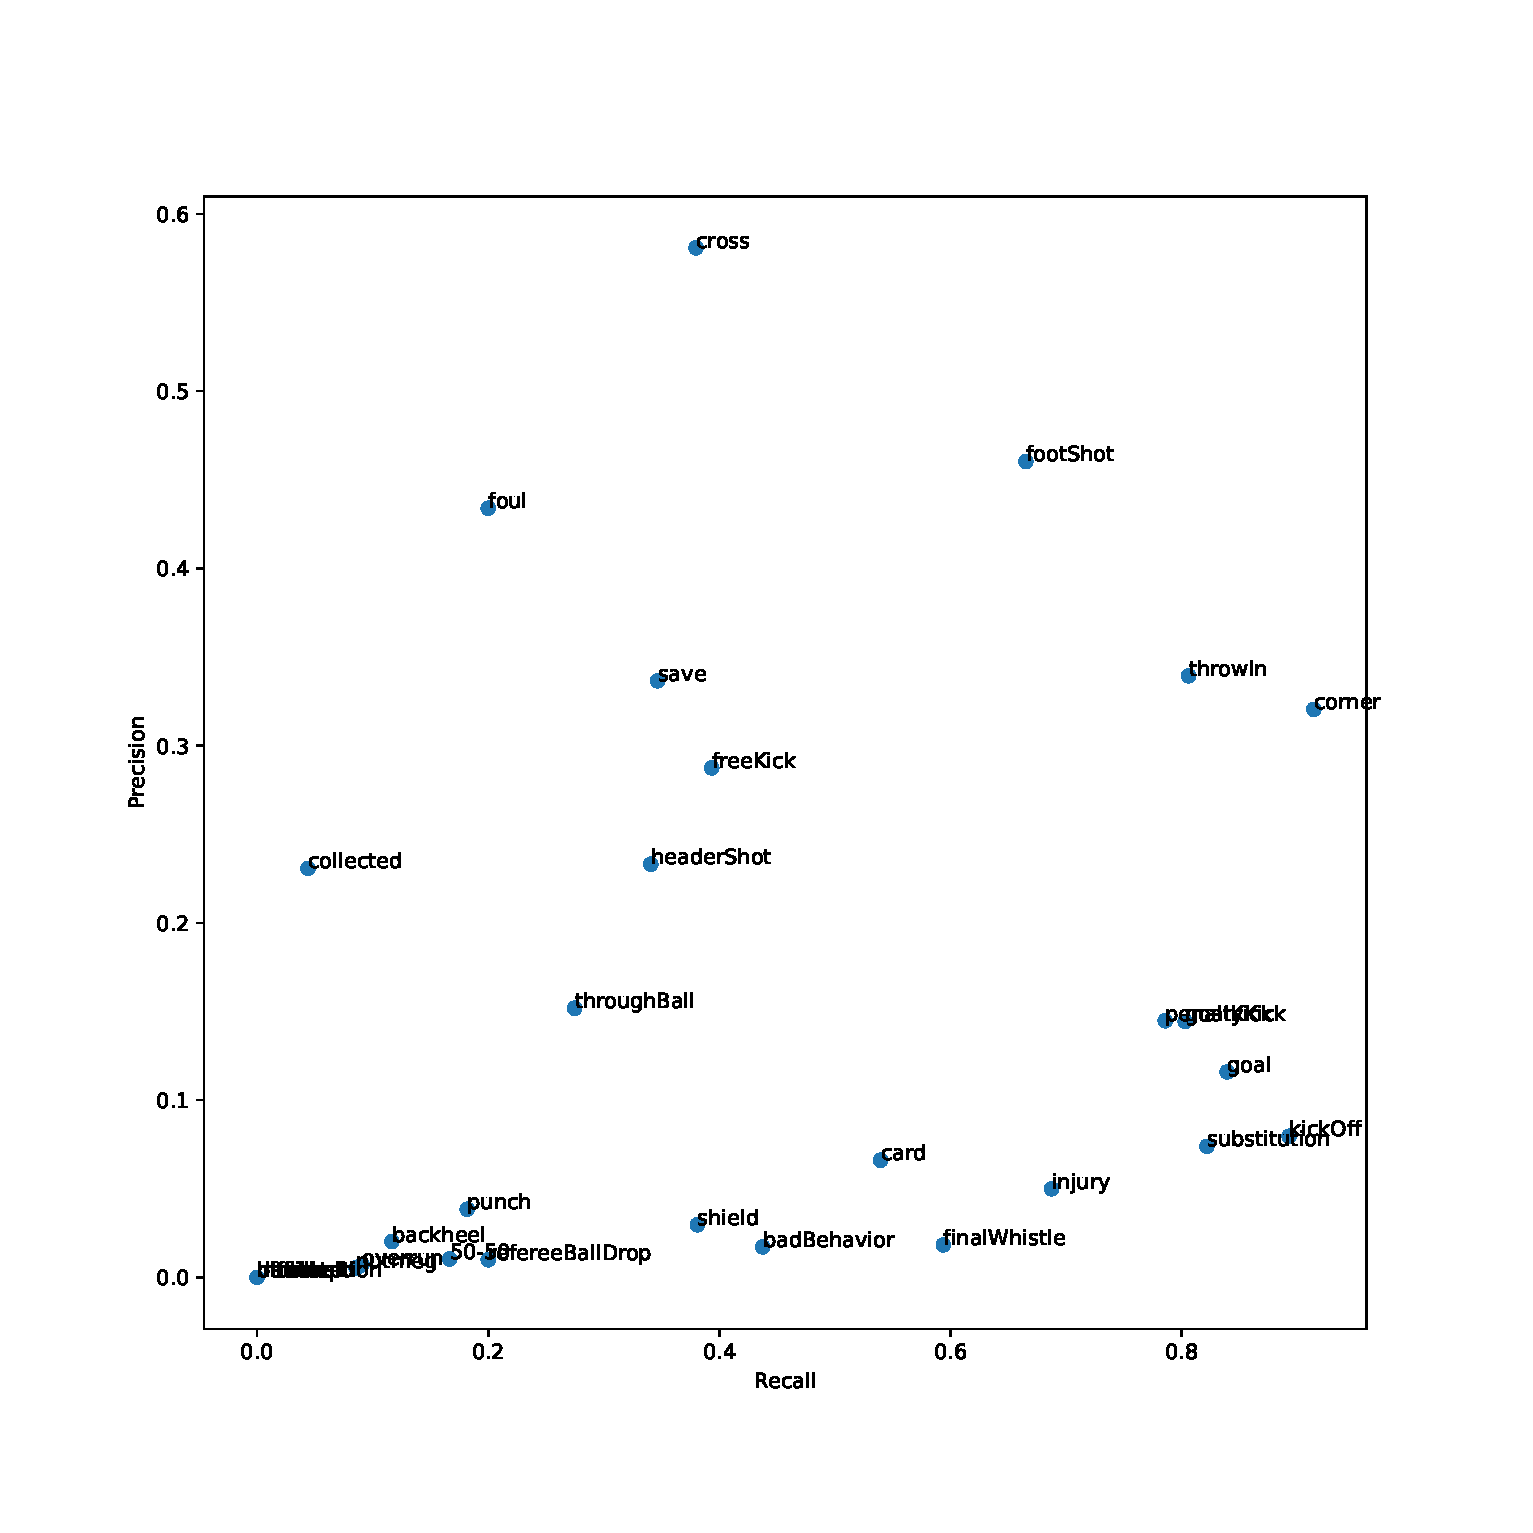
\includegraphics[width=0.99\textwidth, keepaspectratio, interpolate]{img/07_precision_recall_by_class.eps}
%    \caption{Vergleich von Precision und Recall pro Klasse}
%    \label{fig:precision-recall}
%\end{figure}
%\chapter{Integration}
\label{ch:integration}

In diesem Kapitel werden abschließend die notwendigen Schritte zur Integration des \gls{har}-Backbone in direkt nutzbare Umgebung genannt.
Dies schließt die Integration der Action Recognition in eine Temporal Action Detection ein, sowie die Integration der Detection in eine Pipeline zur Verarbeitung neuer ungesehener Videos durch den Nutzer.

\begin{tcolorbox}[title=Todo]
    \begin{itemize}
        \item Intervallbildung mit Grenzwerten out of scope? (Demo nur mit Scores)
        \item Localization: Ergebnisse out of scope?
        \item Localization: Werden Grenzen implizit selbst erlernt?
        \item Deployment: Link einfügen
        \item Die Inbetriebnahme sieht ein iterative Anwendung des \gls{har}-Modells auf konsekutiven Clip-Segmenten eines ungeschnittenen Videos vor.
        \item Die Ergebnisse werden anschließend mit einem naiven Smoothing zur Intervallen transformiert.
        \item Inbetriebnahme eines zusätzliches Modell aus \autoref{sec:temporal-action-detection} zur Temporal Action Detection ist aufgrund des Zeitrahmens nicht vorgesehen.
    \end{itemize}
\end{tcolorbox}

\section{Abbildung auf Zeitintervall}
\label{sec:localization}

Eine Temporal Action Detection wird im Rahmen dieser Arbeit nur naiv umgesetzt indem das \gls{har}-Modell iterativ mit einem Versatz von einer Sekunde auf dem ungeschnittenen Video angewandt wird.
\autoref{fig:detection} zeigt wie sich die Clipsegmente und die damit verbundenen Scores überlagern.

\begin{figure}
    \centering
    \bigimage{fig/detection}{\textwidth}
    \caption{Gantt-Diagramm: Überlagerung der Scores während der Temporal Action Detection}
    \label{fig:detection}
\end{figure}

Jeder Zeitpunkt $t_i$, gibt es abhängig von der Clip-Abdeckung $t_\Delta$ mehrere Clips $\psi \in \Psi$, die sich mit $t_i$ zeitlich überlagern.
Der endgültige Score $\hat{y}_{c \in \gls{tld:A}, t_i}$ einer Klasse ist ergibt sich aus dem Maximum aller Scores überlagernder Clips:

\begin{equation}
    \label{eq:detection}
    \hat{y}_{c \in \gls{tld:A}, t_i} =  \max\limits_{ \psi \in \Psi } y_{c, t_i, \psi} \times \text{overlap}([t_\psi, t_\psi + t_\Delta ], [t_i, t_i + 1]) \times \text{influence}(\frac{t_{\psi, i}}{t_\Delta})
\end{equation}

Die Hilfsfunktion $\text{overlap}$ (\autoref{eq:overlap}) filtert alle Clips ohne Überschneidung mit der jeweiligen Videosekunde heraus, während die die Funktion $\text{influence}$ Scores geringer gewichtet, deren Clip sich nur ganz am Anfang oder ganz am Ende mit der gesuchten Videosekunde überschneidet.

\begin{equation}
    \label{eq:overlap}
    \text{overlap}(t_1, t_2) = t_1^1 \leq t_2^2 \land t_2^1 \geq t_1^2
\end{equation}

\begin{equation}
    \label{eq:influence}
    \text{influence}(x) =  \max \{0, -9{(x-0.5)}^4 + 1\}
\end{equation}

Aus den resultierenden Scores  $\hat{y}_{t_i}$ können mithilfe von neuen Grenzwerten feste Intervalle geformt werden, was jedoch nicht dem Umfang dieser Arbeit entspricht.
Zudem wird angemerkt, dass eine auf Intervallen basierte Evaluierung mit Metriken wie tIoU (temporal Intersection over Union) zu Ergebnissen mit einem geringen Informationsgehalt führt, da die zeitlichen Ground-Truth-Intervall nicht manuell erstellt und validiert wurden.

%\subsection{Evalutierung für temp. Action Localization}
%* Sparsity Concentration Index (SCI) \cite{Sun15}
%1. sample M pairs of video Frames for each sequence
%2. final score $p_i$ for class $i$ is depending on entropy

\section{Inference-Pipeline}
\label{sec:inference-pipeline}

Um das \gls{har}-Modell in der realen Welt einzusetzen, wird eine Anwendung bereitgestellt, die ungeschnittene Videos verarbeiten kann.
In der Anwendung kann der Nutzer ein Video wahlweise hochladen oder einen YouTube-Link zu dem Video angeben.
Zusätzlich kann eins der vortrainierten Modelle und ein Klassifikationsgrenzwert ausgewählt werden.

Mit Absenden des Daten wird das Video lokal hoch- \bzw heruntergeladen, analysiert und in Clips segmentiert.
Anschließend wird, wie zuvor beschrieben, das \gls{har}-Modell inferiert und die Scores anschließend für jeden Zeitpunkt aggregiert.

Auf Basis des vom Nutzer angegebenen Grenzwerts können nur die Annotationen (im gleichen Format wie die JSON-Datenbank der Trainingsdaten) heruntergeladen werden.
Alternativ kann auch ein Ausschnitt des Video mit eingebrannten Scores heruntergeladen werden.
\autoref{fig:inference-pipeline} zeigt den kompletten Ablauf.

\begin{figure}
    \centering
    \bigimage{fig/inference}{0.8\textwidth}
    \caption{Aktivitätsdiagramm: Inferenz-Pipeline}
    \label{fig:inference-pipeline}
\end{figure}

Die während des Trainings erforderlichen Schritte des zufallsbasierten Samplings entfällt an dieser Stelle, da eben alle Zeitpunkte des Videos erfasst werden sollen.
Auch der Schritt zur Data Augmentation wird hier nicht mehr benötigt und würde die Inferenz nur zusätzlich erschweren.

\section{Deployment}



\chapter{Zusammenfassung}
\label{ch:zusammenfassung}

Zum Ende dieser Arbeit wird noch einmal der Umfang und die Ergebnisse rekapituliert.
Darüber hinaus wird ein Ausblick gegeben, wie sich die Ergebnisse durch weitere Schritte verbessern ließen und eine Einschätzung ob die angewandten Methoden dieser Arbeit das Ziel erreichen konnten.

\begin{tcolorbox}[title=Todo]
 \begin{itemize}
  \item Ergebnisse in Rekapitulation einbauen
 \end{itemize}
 \end{tcolorbox}

\section{Rekapitulation}
\label{sec:rekapitulation}

Um Video Understand im Fußball-Sektor gibt es bis dato kein umfangreiches Datenset mit mehr als zehn Klassen.
Im Zuge dieser Arbeit wurde ein mächtigeres Datenset mit insgesamt 32 Spielaktionsklassen auf Basis öffentlich zugänglicher Daten erstellt.
Durch die Verfügbarkeit dieses neuen Datensets, konnte moderne Deep Learning Modelle zu Multi-Label Action Recognition trainiert werden, deren Ergebnisse nicht hinter den Ergebnissen vorangegangener Datensets zurückbleiben.

Im Zuge des Training wurden Modelle aus den Kategorien 3D-Convolution und faktorisierter 3D-Convolution getestet und herausgearbeitet welche Samplingstrategie für die jeweilige Kategorie am besten geeignet ist.
Darüber hinaus konnte auf Basis der Rechenergebnisse eine umfassende Analyse der Aktionsklassen durchgeführt werden, die Spielaktionen bestimmte Schwierigkeitsgrade zugeteilt.

%todo: was ist jetzt am besten? wie gut genau und was ist leicht und was ist schwer?

\section{Ausblick}
\label{sec:ausblick}

Die Rechenergebnisse dieser Arbeit stellen eine solide Baseline zukünftiger Arbeiten dar, die durch zusätzlichen Aufwand noch viel Verbesserungspotential hat.
Offensichtlich lassen sich noch bessere Ergebnisse erziehen, wenn das vorgestellte Baseline-Modell von Grund auf mit den neuen Datenset trainiert würde, was aus Hardware-Beschränkungen im Rahmen dieser Arbeit nicht möglich war.
Weitere Fortschritte sind denkbar durch die Hinzunahme der Audiosignale der zugrunde liegenden Videos.
Ein ähnlicher Ansatz wurde bereits in \cite{Wang19} beschrieben.
Ebenso vielversprechend ist die in \cite{Wu20} vorgestellte Methodik die räumliche Auflösung während des Trainings von niedrig- zu höher auflösenden Samples zu variieren.

Mehrschrittige Modell, die aufgrund des erhöhten Entwicklungsaufwand im Vorfeld ausgeschlossen wurden, könnten ebenfalls Fortschritte bringen.
So könnten \zB vorab Kamerawechsel erkannt werden und Clips ausschließlich so gesamplet werden, dass sie kontinuierliche Bewegung ohne Kameraschnitte zeigen.
Alternative kann die Information eines Kamerawechsels, wie auch weitere separat erhobene Informationen wie Ballposition oder Spielerkoordinaten in das Baseline-Modell einfließen.

Im Anschluss an die Action Recognition kann die hier nur naiv umgesetzte Temporal Action Detection durch den Einsatz eines mächtigeren Modells aus \autoref{sec:temporal-action-detection} ersetzt werden, die mit genaueren Annotationen eines abgewandelten Datensets trainiert werden können.

Zusätzlich kann auf der selben Datengrundlage (mit gleichen Spielen) ein Datenset mit Spielerkoordinaten und Identifiern erstellt werden.
Mit solchen Daten kann \ggf ein Modell zum Tracking von Spielern oder sogar der Projizierung von Spielern auf Spielfeldkoordinaten erstellt werden und mit dem hier vorgestellten Modell zur Aktionserkennung verknüpft werden.
So wäre eine vollständige Erfassung Spieler-bezogenen Statistiken auf Basis von Spielaktionen und Spielerpositionen möglich, die das Fußball-Scouting nachhaltig prägen könnte.

\section{Fazit}
\label{sec:fazit}

Abschließend lassen sich die Fragestellungen aus \autoref{sec:forschungsfrage} beide mit \emph{Ja} beantworten.
Die Lernbarkeit von bis zu 32 wurde im Zuge zahlreicher Experimente mehrmals bewiesen.
Als besonders anspruchsvoll gelten hierbei \dots

% todo: zweite frage

Auch der produktive Einsatz der Action Recognition in eine Anwendung zur Temporal Action Detection war möglich.
Aufgrund zu ungenauer Intervallgrenzen in dem neu erhobenen Datenset, konnte der Erfolg der Detection nicht quantifiziert werden.
Jedoch werden die Ergebnisse (subjektiv) für anwendbar befunden.


% Anhang
\cleardoublepage
\appendix
\chapter{Rechenergebnisse von HAR-Modellen in der Literatur}
\label{ch:leaderboard}

\autoref{tab:models} zeigt die publizierten Rechenergebnisse der in \autoref{ch:sota} vorgestellten Modelle im Vergleich.
Die Ergebnisse von UCF-101 beziehen sich alle auf die als 3-fold-Accuracy angegebene Metrik.
Sports-1M zeigt jeweils die Accuracy im Format \emph{clip@1}/\emph{video@1} und Kinetics stets die Top-1-Accuracy.

\begin{figure}
    \csvautotabular{tbl/models.csv}
    \label{tab:models}
\end{figure}

\chapter{Aktionskatalog}
\label{ch:aktionskatalog}

In \autoref{tab:action} werden alle 32 Klassen des im Rahmen dieser Arbeit generierten und in \autoref{ch:data} vorgestellten Datensets aufgelistet.
Neben der Anzahl ist die durchschnittliche und maximaler Dauer pro Aktion vermerkt, die sich aus den \gls{annotationen} in \cite{Statsbomb20} ergeben.
Aktionen, die hier keinen Wert vorweisen werden lediglich als Zeitpunkt in \gls{sbod} repräsentiert.

\begin{figure}
    \centering
    \begin{subfigure}{0.45\textwidth}
        \centering
        \csvautotabular{tbl/actions_a.csv}
    \end{subfigure}
    \begin{subfigure}{0.45\textwidth}
        \centering
        \csvautotabular{tbl/actions_b.csv}
    \end{subfigure}
    \label{tab:action}
\end{figure}

\chapter{Paarweise Intersektion von Spielaktionen}
\label{ch:overlaps}

In \autoref{fig:overlaps} wurde für alle 32 Klassen der prozentuale Anteil aller Sampler einer Klasse berechnet der jeweils in Kombination mit einer anderen Klasse auftritt.
Ein Eintrag $c_{ij}$ lässt sich wie folgt interpretieren:
$c_{ij}$ \% aller Samples der Klasse $i$ treten gemeinsam mit der der Klasse $j$ auf.

Wie man sieht, ereignen sich \zB 74 \% der Aktionen \code{saved} (innerhalb eines Zeitkontextes von $\Delta=4$ Sekunden) gleichzeitig mit Aktionen der Klasse \code{footShot}.
Bei einer niedrigeren Wahl von $\Delta$ sind die Abhängigkeiten entsprechend geringer, es treten jedoch die gleichen Kombinationen hoher Abhängigkeiten auf.

\begin{figure}
    \centering
    \bigimage{img/data-plots/4sec/pairwise_occurrences_all_202010-1419-3817}{\textwidth}
    \caption{Anteil paarweiser Überschneidungen pro Klasse (hier: $\Delta = 4$)}
    \label{fig:overlaps}
\end{figure}



% DON'T set \bibliographystyle here -- use the documentclass option instead
%\bibliographystyle{abbrv}

\printbibliography[heading=bibintoc]

% Glossar
\cleardoublepage
\printglossary[type=\acronymtype, title=Abkürzungsverzeichnis, toctitle=Abkürzungsverzeichnis]
\printglossary[title=Glossar, toctitle=Glossar]
\printglossary[type=symbols, title=Symbolverzeichnis, toctitle=Symbolverzeichnis]


\closing %%%%%%%%%%%%%%%%%%%%%%%%%%%%%%

\end{document}
